\documentclass[10pt]{article}  

%%%%%%%% PREÁMBULO %%%%%%%%%%%%
\title{Plantilla para prácticas de UPIITA}
\usepackage[spanish]{babel} %Indica que escribiermos en español
\usepackage[utf8]{inputenc} %Indica qué codificación se está usando ISO-8859-1(latin1)  o utf8  
\usepackage{amsmath} % Comandos extras para matemáticas (cajas para ecuaciones,
% etc)
\usepackage{amssymb} % Simbolos matematicos (por lo tanto)
\usepackage{graphicx} % Incluir imágenes en LaTeX
\usepackage{color} % Para colorear texto
\usepackage{subfigure} % subfiguras
\usepackage{float} %Podemos usar el especificador [H] en las figuras para que se
% queden donde queramos
\usepackage{capt-of} % Permite usar etiquetas fuera de elementos flotantes
% (etiquetas de figuras)
\usepackage{sidecap} % Para poner el texto de las imágenes al lado
	\sidecaptionvpos{figure}{c} % Para que el texto se alinie al centro vertical
\usepackage{caption} % Para poder quitar numeracion de figuras
\usepackage{commath} % funcionalidades extras para diferenciales, integrales,
% etc (\od, \dif, etc)
\usepackage{cancel} % para cancelar expresiones (\cancelto{0}{x})
 
\usepackage{anysize} 					% Para personalizar el ancho de  los márgenes
\marginsize{2cm}{2cm}{2cm}{2cm} % Izquierda, derecha, arriba, abajo

\usepackage{appendix}
\renewcommand{\appendixname}{Apéndices}
\renewcommand{\appendixtocname}{Apéndices}
\renewcommand{\appendixpagename}{Apéndices} 

% Para que las referencias sean hipervínculos a las figuras o ecuaciones y
% aparezcan en color
\usepackage[colorlinks=true,plainpages=true,citecolor=blue,linkcolor=blue]{hyperref}
%\usepackage{hyperref} 
% Para agregar encabezado y pie de página
\usepackage{fancyhdr} 
\pagestyle{fancy}
\fancyhf{}
\fancyhead[L]{\footnotesize UGR} %encabezado izquierda
\fancyhead[R]{\footnotesize DOM}   % dereecha
\fancyfoot[R]{\footnotesize Memoria}  % Pie derecha
\fancyfoot[C]{\thepage}  % centro
\fancyfoot[L]{\footnotesize Master en Ingeniería Informática}  %izquierda
\renewcommand{\footrulewidth}{0.4pt}

% Directorio para las imágenes
\graphicspath{{/Users/jesusgarciamanday/Desktop/Master/DOM/Practicas/Memoria/Imagenes/}}


\usepackage{listings} % Para usar código fuente
\definecolor{dkgreen}{rgb}{0,0.6,0} % Definimos colores para usar en el código
\definecolor{gray}{rgb}{0.5,0.5,0.5} 
% configuración para el lenguaje que queramos utilizar
\lstset{language=Matlab,
   keywords={break,case,catch,continue,else,elseif,end,for,function,
      global,if,otherwise,persistent,return,switch,try,while},
   basicstyle=\ttfamily,
   keywordstyle=\color{blue},
   commentstyle=\color{red},
   stringstyle=\color{dkgreen},
   numbers=left,
   numberstyle=\tiny\color{gray},
   stepnumber=1,
   numbersep=10pt,
   backgroundcolor=\color{white},
   tabsize=4,
   showspaces=false,
   showstringspaces=false}

\newcommand{\sen}{\operatorname{\sen}}	% Definimos el comando \sen para el seno
%en español

%%%%%%%% TERMINA PREÁMBULO %%%%%%%%%%%%

\begin{document}

%%%%%%%%%%%%%%%%%%%%%%%%%%%%%%%%%% PORTADA %%%%%%%%%%%%%%%%%%%%%%%%%%%%%%%%%%%%%%%%%%%%
																					%%%
\begin{center}																		%%%
\newcommand{\HRule}{\rule{\linewidth}{0.5mm}}									%%%\left
 																					%%%
\begin{minipage}{0.48\textwidth} \begin{flushleft}
%
\includegraphics[scale = 0.63]{Imagenes/logo_upiita}
\end{flushleft}\end{minipage}
\begin{minipage}{0.48\textwidth} \begin{flushright}
%
\includegraphics[scale = 0.35]{Imagenes/IPN}
\end{flushright}\end{minipage}

													 								%%%
\vspace*{0.25cm}								%%%
																					%%%	
\textsc{\huge Universidad de Granada}\\[1.5cm]	

\textsc{\LARGE Master en Ingeniería Informática}\\[1.5cm]													%%%

\textsc{\LARGE Domótica}\\[1.5cm]													%%%

\begin{minipage}{0.9\textwidth} 
\begin{center}																					%%%
\textsc{\LARGE KNX}
\end{center}
\end{minipage}\\[0.5cm]
%%%
    																				%%%
 			\vspace*{1cm}																		%%%
																					%%%
\HRule \\[0.4cm]																	%%%
{ \huge \bfseries Memoria de las prácticas}\\[0.4cm]	%%%
 																					%%%
\HRule \\[1.5cm]																	%%%
 																				%%%
																					%%%
\begin{minipage}{0.46\textwidth}													%%%
\begin{flushleft} \large															%%%
\emph{Autor:}\\	
 Manuel Jesús García Manday
%%%
			%\vspace*{2cm}	
            													%%%
										 						%%%
\end{flushleft}																		%%%
\end{minipage}		
																%%%
\begin{minipage}{0.52\textwidth}		
\vspace{-0.6cm}											%%%
\begin{flushright} \large															%%%													%%%
\end{flushright}																	%%%
\end{minipage}	
\vspace*{1cm}
%\begin{flushleft}
 	
%\end{flushleft}
%%%
 		\flushleft{\textbf{\Large Master en Ingeniería Informática}	}\\																		%%%
\vspace{2cm} 																				
\begin{center}																					

%{\large \today}																	%%%
 			\end{center}												  						
\end{center}							 											
																					
\newpage																		
%%%%%%%%%%%%%%%%%%%% TERMINA PORTADA %%%%%%%%%%%%%%%%%%%%%%%%%%%%%%%%

\tableofcontents 

\newpage

\section{Objetivo.}

El objetivo de este documento es presentar una memoria sobre la realización de las prácticas de la asignatura. A través del mismo se describirán los pasos empleados para el desarrollo de cada una de las prácticas propuestas así como las herramientas utilizadas para ello. Para el desarrollo de las mismas se va a emplear el software \textbf{ETS5} como entrono de desarrollo integrado (IDE) y el sistema \textbf{KNX} como entorno de pruebas y despliegue de los diferentes proyectos, con el fin de realizar la implementación y pruebas pertinentes para probar que el comportamiento obtenido por las distintas funcionalidades de las prácticas es el correcto. 


\section{Configuración del sistema.} 
Una vez que se ha instalado el software \textbf{ETS5} para programar el equipo de prácticas KNX, es necesario importar las pertinentes librerías de cada uno de los módulos para su posterior uso como se muestra en la siguiente imagen. \\

\begin{figure}[H]
	\begin{center}
	 		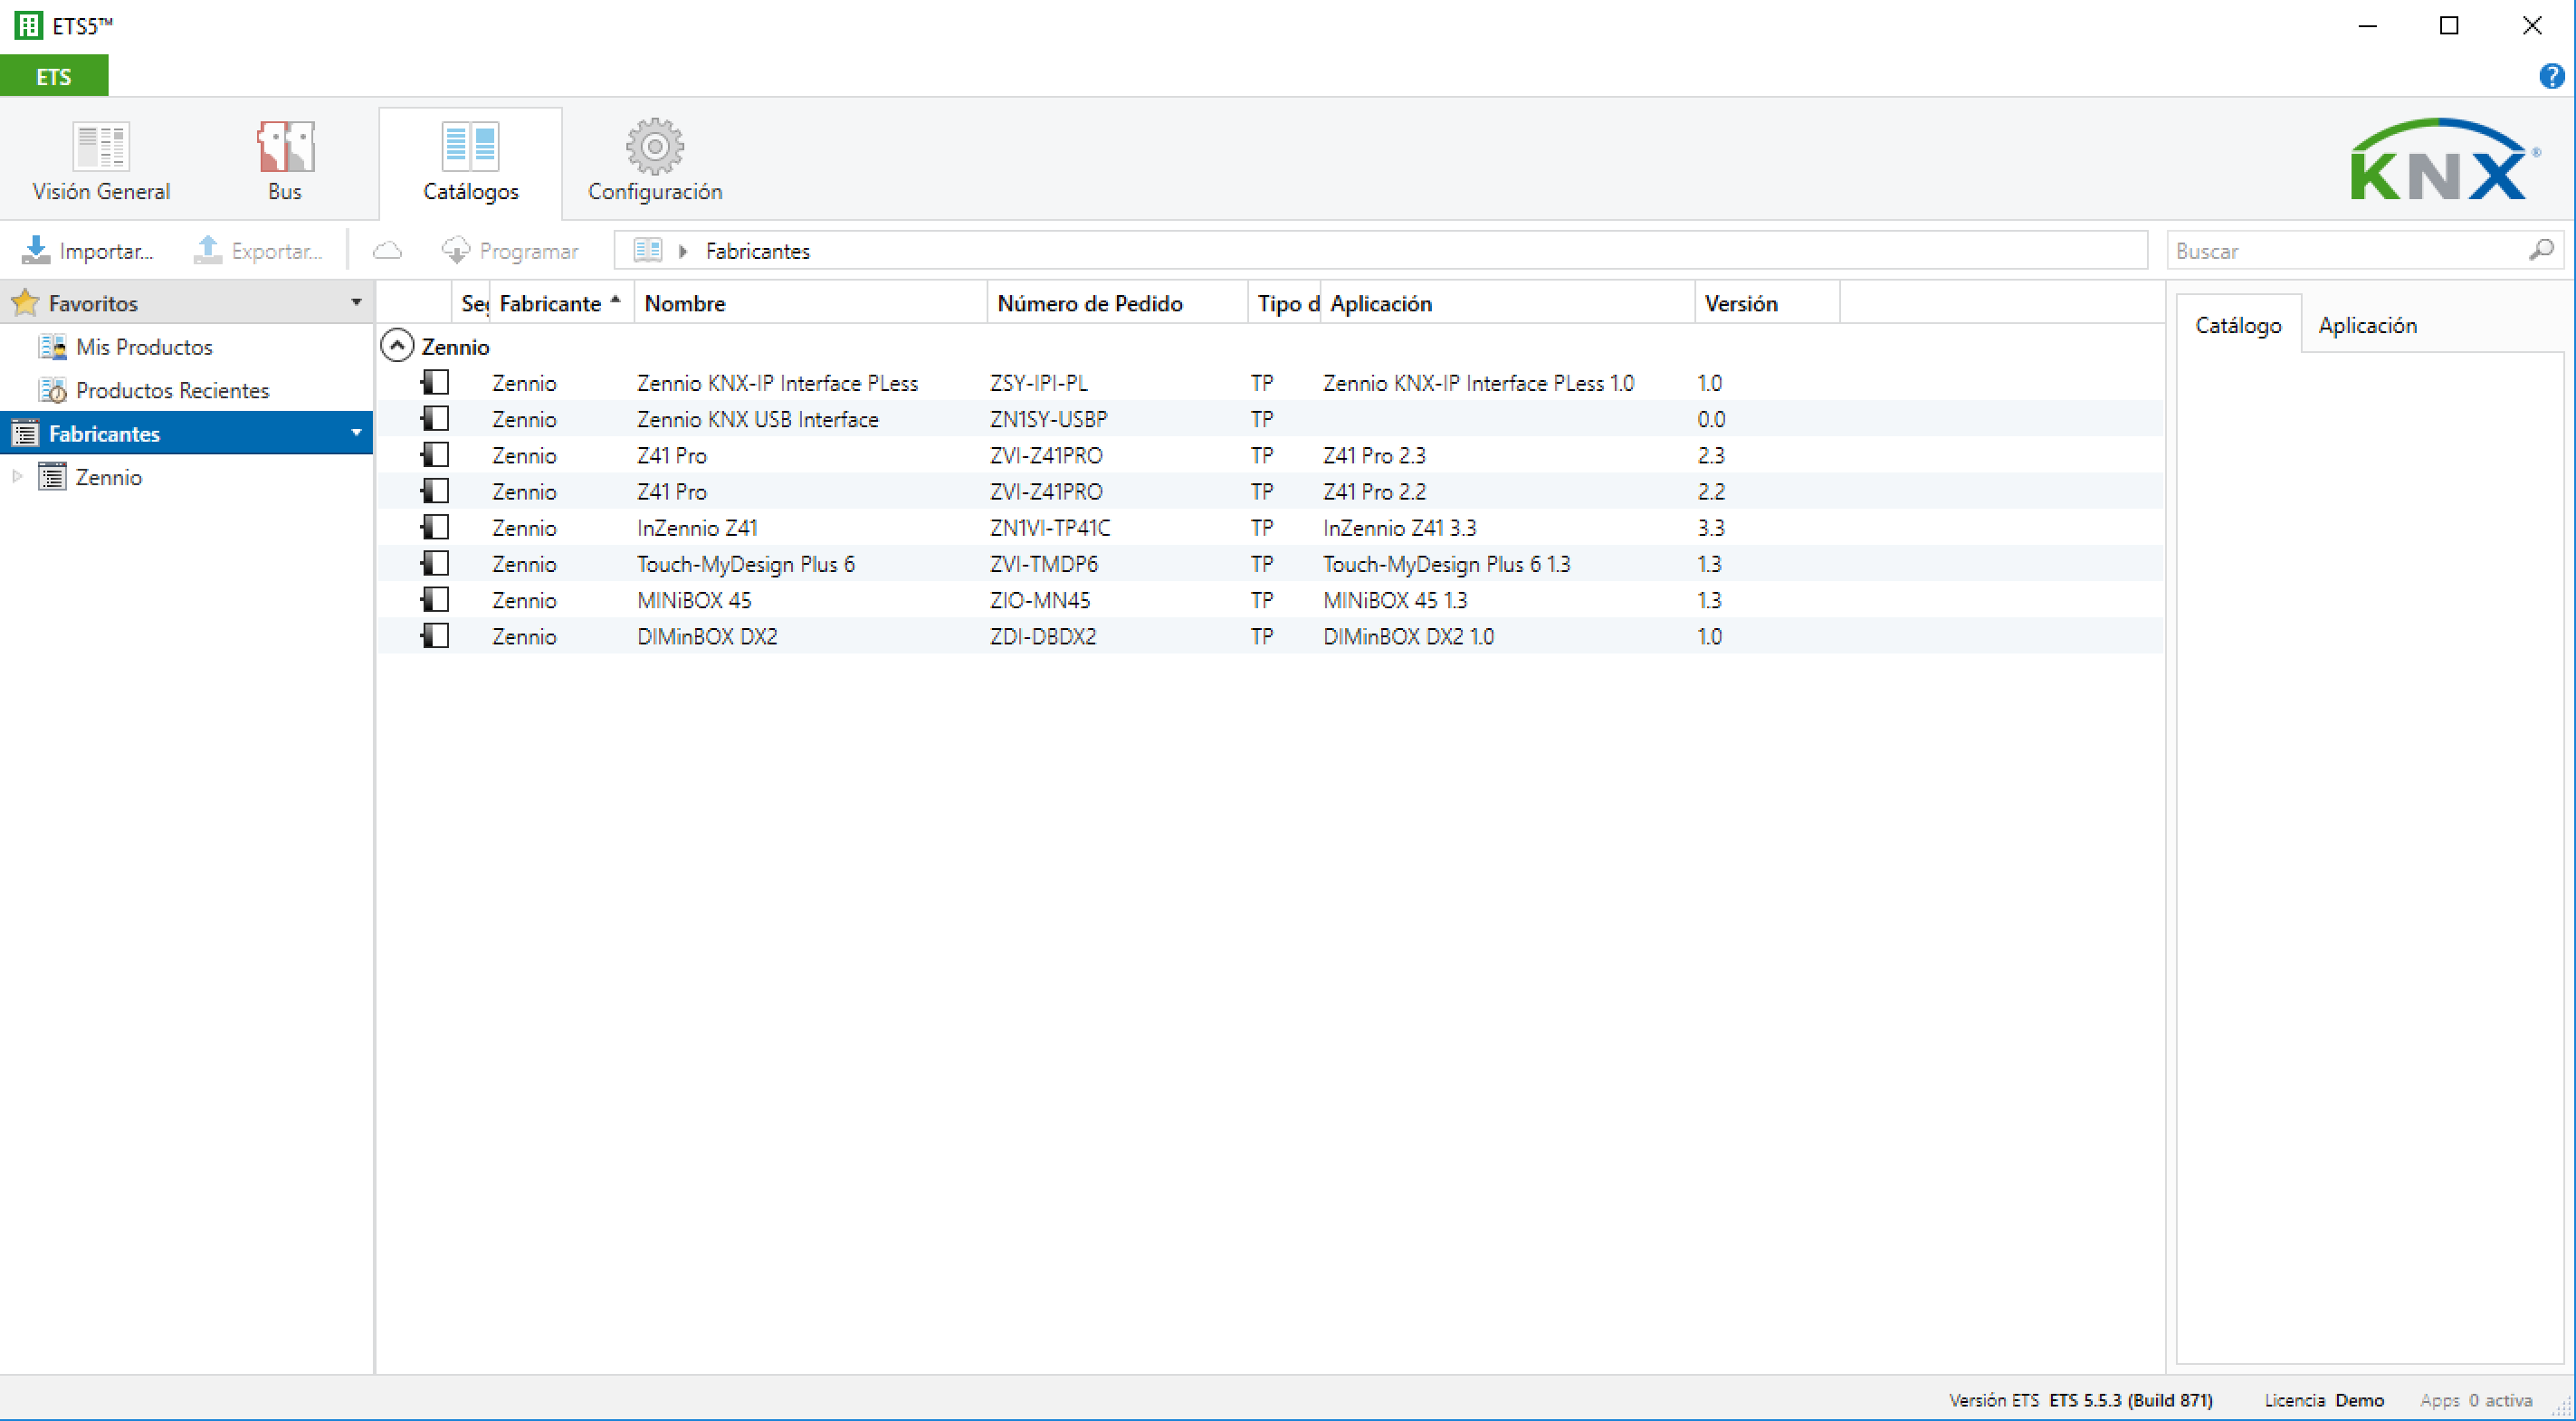
\includegraphics[width = 1.00\textwidth]{Imagenes/img1}
 		\captionof{figure}{\label{fig:IPN}Importando librerías.} 
	\end{center} 
\end{figure}

Ya esta el software preparado para comenzar a programar con los módulos del equipo de prácticas KNX en función de las necesidades que tenga cada situación como se irán describiendo en los siguientes puntos. \\


\section{Práctica 1. Regulación de luz.} 
La finalidad de esta primera práctica es la de realizar una funcionalidad que sea capaz de regular la intensidad luminosa de una lámpara led a través del módulo de botonera táctil. Para el desarrollo de esta primera situación se van a utilizar los módulos \textbf{DIMinBOX DX2} y \textbf{Touch-MyDesign Plus 6} del equipo KNX, por lo que los agregamos a nuestros dispositivos. El dispositivo \textbf{DIMinBOX DX2} se situará en el armario, mientras que el \textbf{Touch-MyDesign Plus 6} se colocará en el salón como se muestra en la siguiente figura. \\

\begin{figure}[H]
	\begin{center}
	 		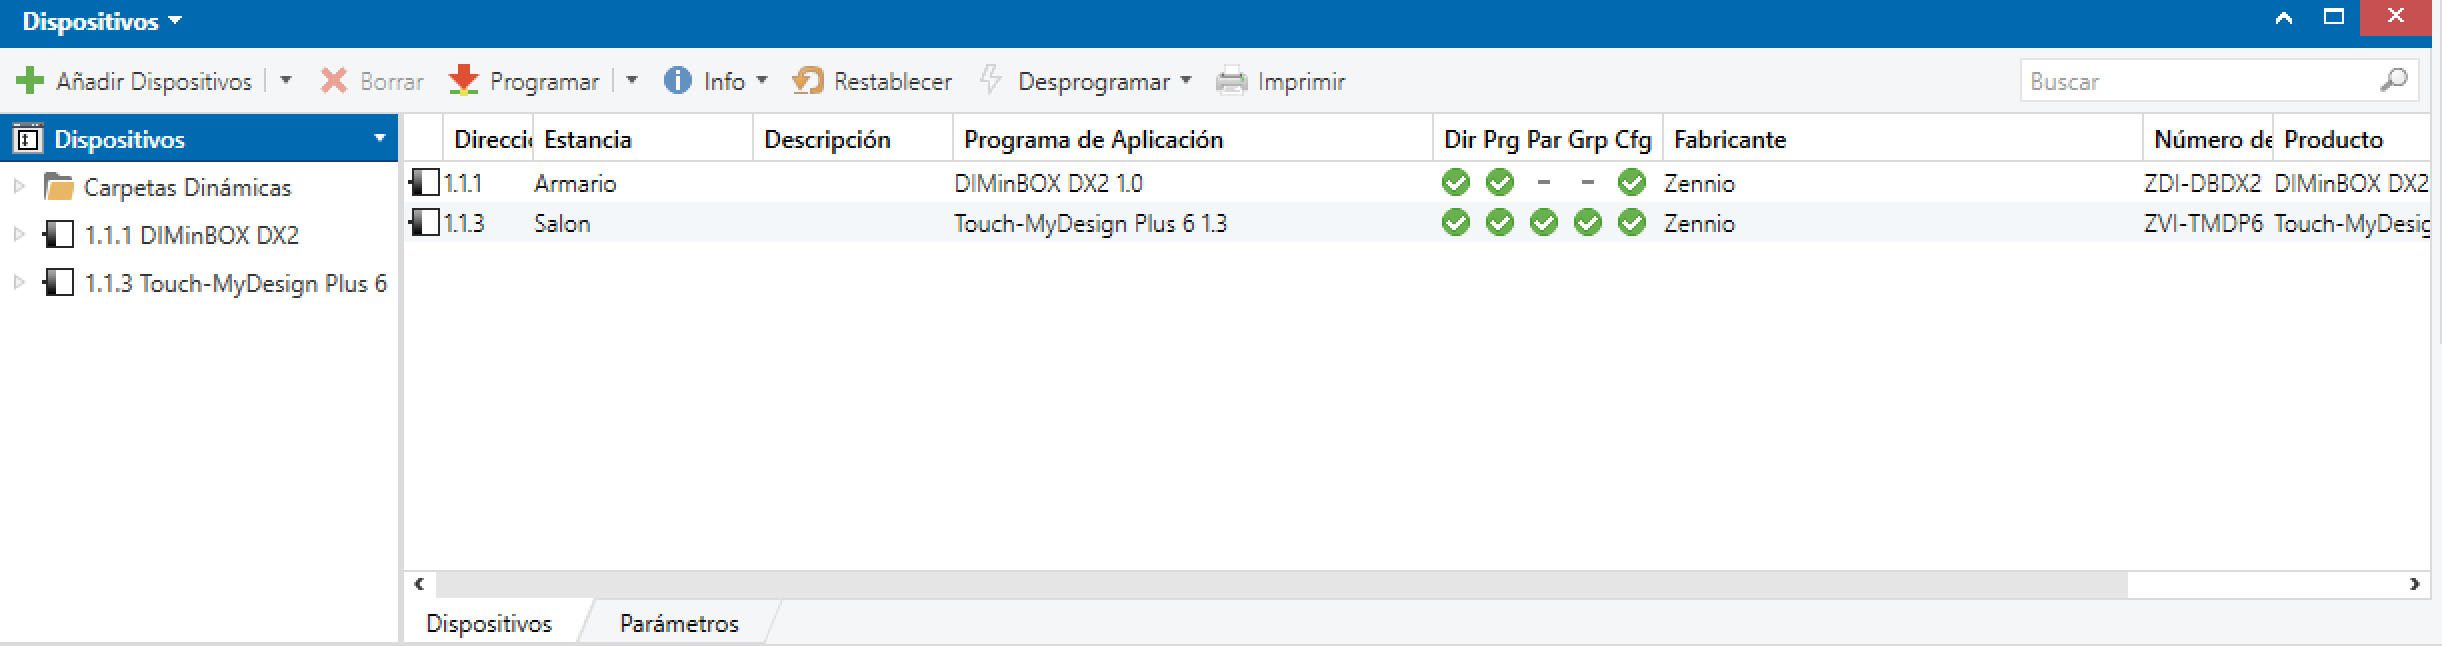
\includegraphics[width = 1.00\textwidth]{Imagenes/img2}
 		\captionof{figure}{\label{fig:IPN}Agregando dispositivos.} 
	\end{center} 
\end{figure}

Con los dispositivos agregados pasamos a configurar sus parámetros. El  \textbf{DIMinBOX DX2} dispone de dos salidas \textbf{C1} y \textbf{C2} que se encuentran conectadas a dos lámparas led de 220V, para nuesto supuesto vamos a utilizar las dos para controlar la regulación de la luz. \\

\begin{figure}[H]
	\begin{center}
	 		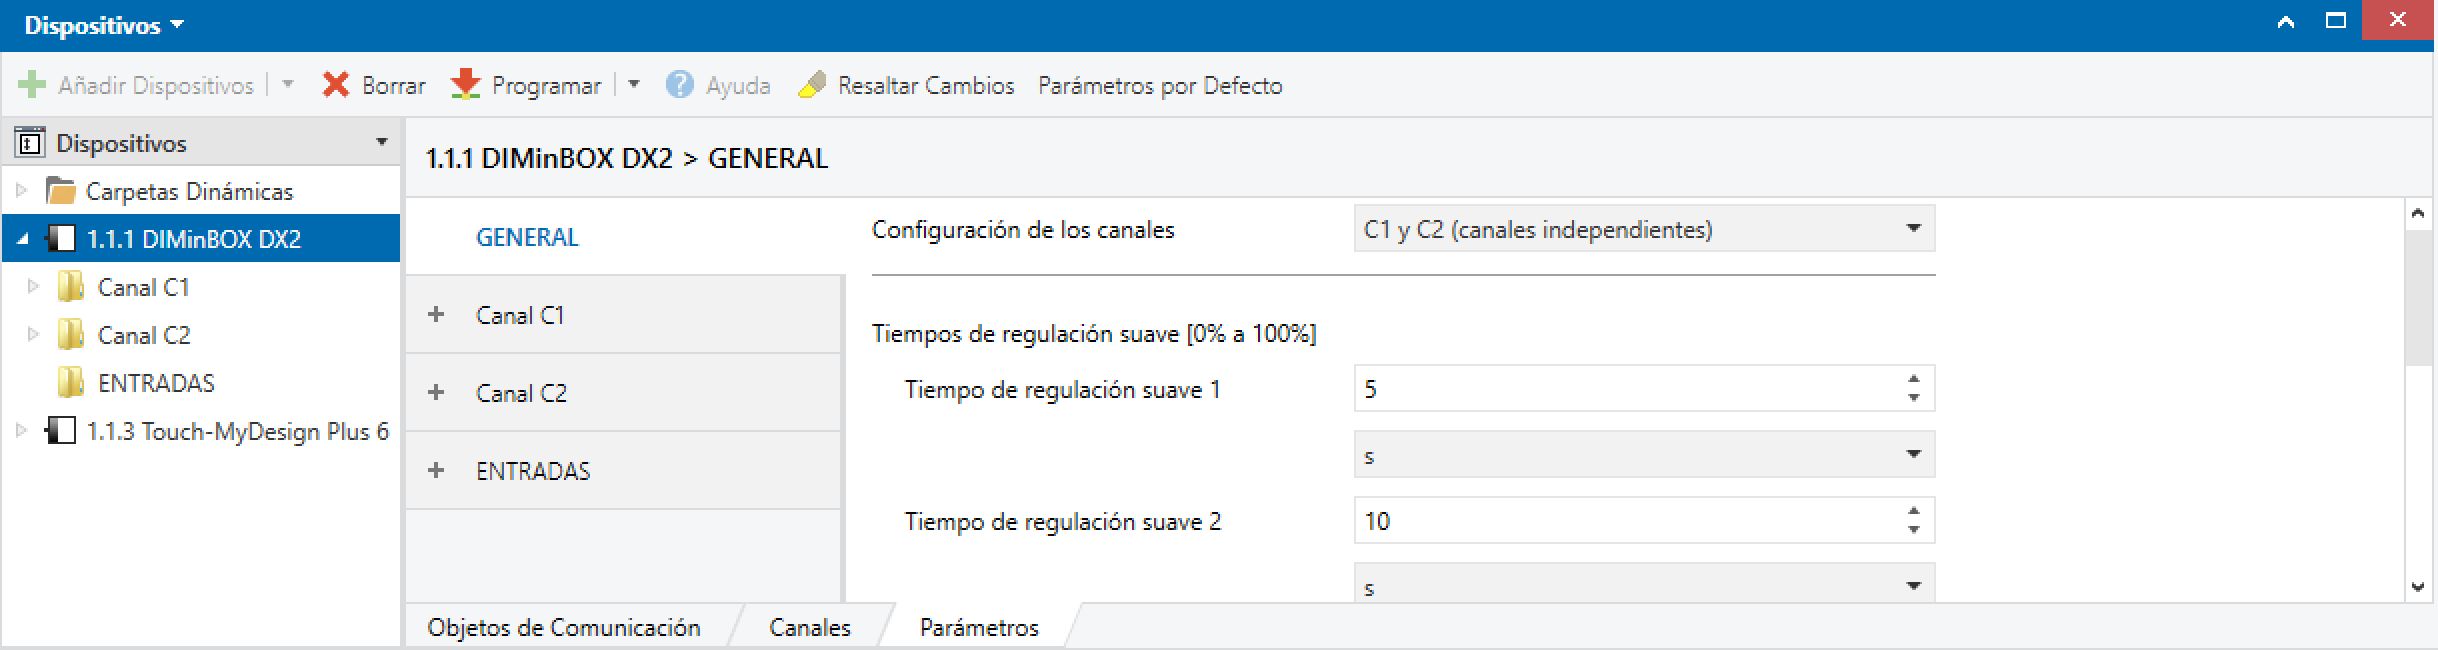
\includegraphics[width = 1.00\textwidth]{Imagenes/img3}
 		\captionof{figure}{\label{fig:IPN}Configurando parámetros del \textbf{DIMinBOX DX2}.} 
	\end{center} 
\end{figure}

Una vez que se han configurado los parámetros de dicho dispositivo, podemos ver los objetos de comunicación de los que dispone cada uno de las dos entradas del citado módulo. \\

\begin{figure}[H]
	\begin{center}
	 		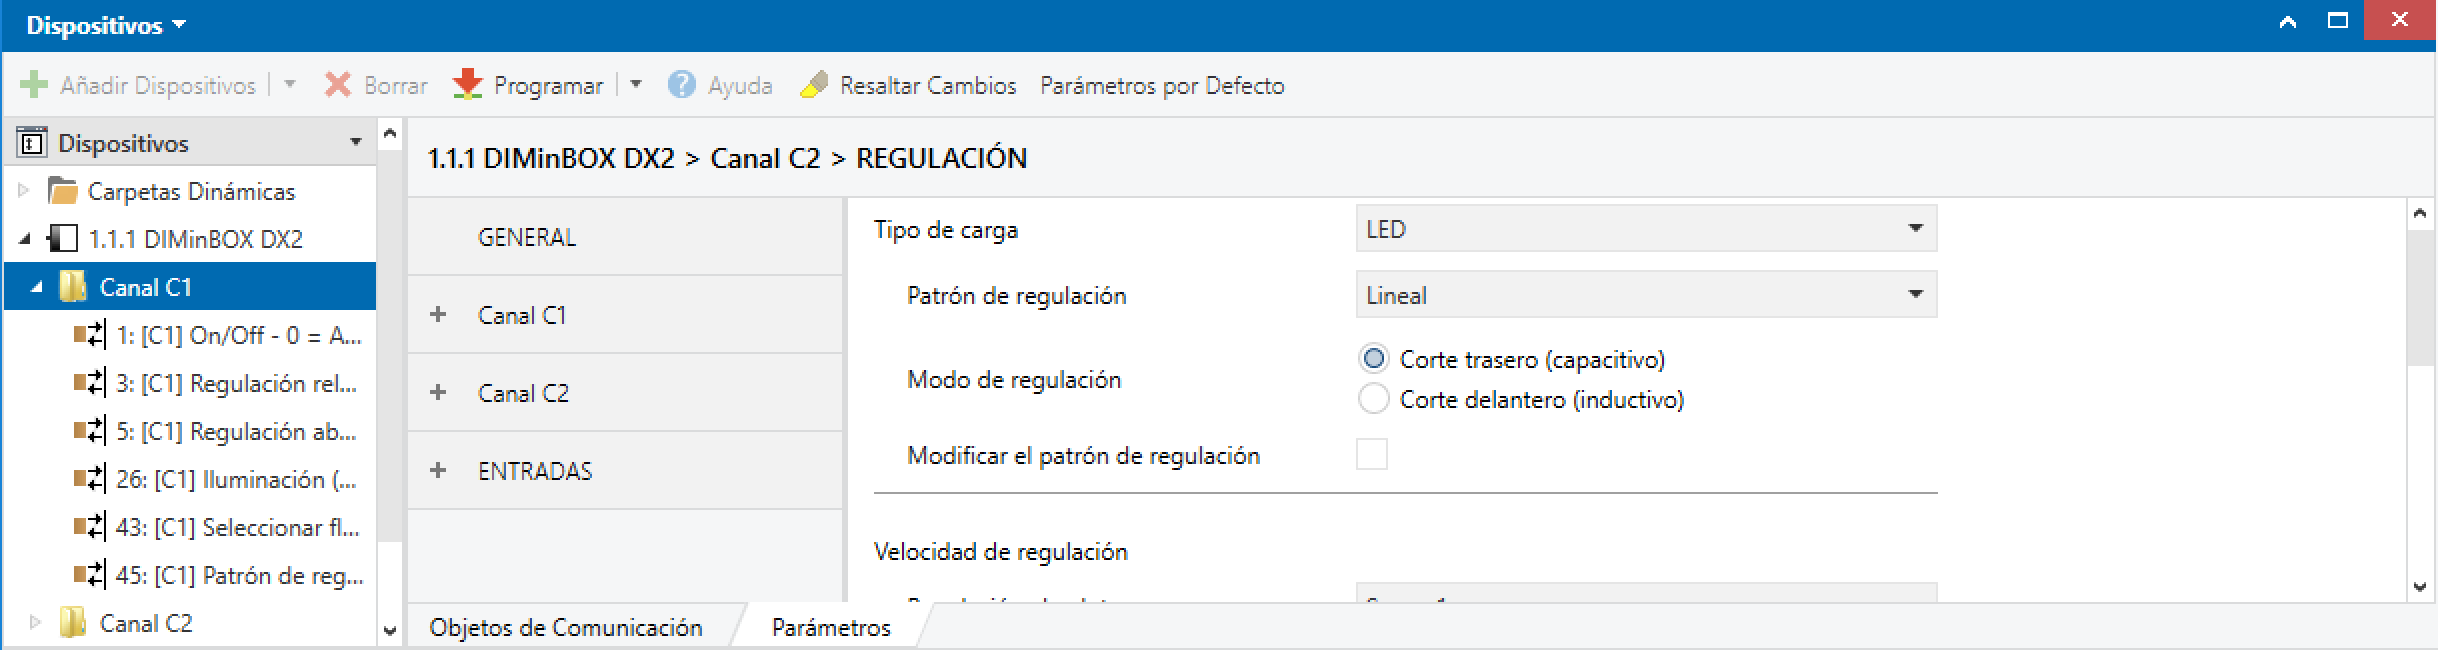
\includegraphics[width = 1.00\textwidth]{Imagenes/img4}
 		\captionof{figure}{\label{fig:IPN}Objetos de comunicación para \textbf{C1}.} 
	\end{center} 
\end{figure}

\begin{figure}[H]
	\begin{center}
	 		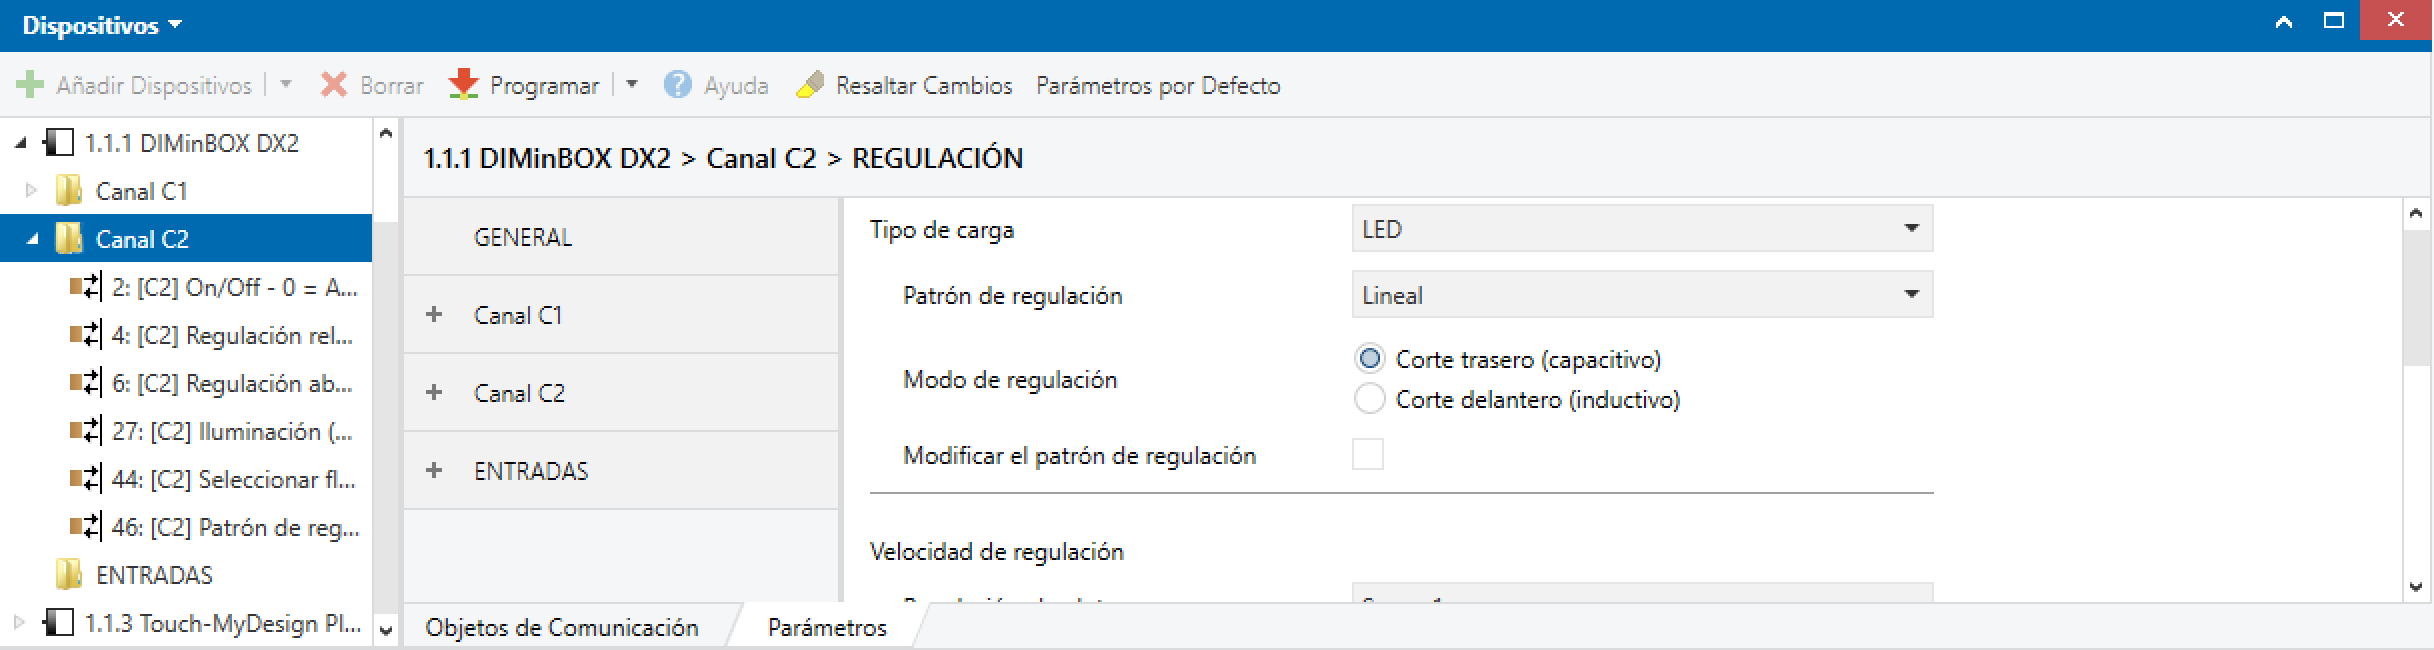
\includegraphics[width = 1.00\textwidth]{Imagenes/img5}
 		\captionof{figure}{\label{fig:IPN}Objetos de comunicación para \textbf{C2}.} 
	\end{center} 
\end{figure}

Ahora es el turno de configurar los parámetros del módulo \textbf{Touch-MyDesign Plus 6}. Para este dispositivo configuraremos uno de los pulsadores principales (\textbf{A1}) al cual le daremos una función de ``binario'' junto a una acción de ``conmutador''. En cuanto a la pareja B de este pulsador principal le estableceremos una función de ``control de regulador'' así como un paso de regulación del 25\%. \\

\begin{figure}[H]
	\begin{center}
	 		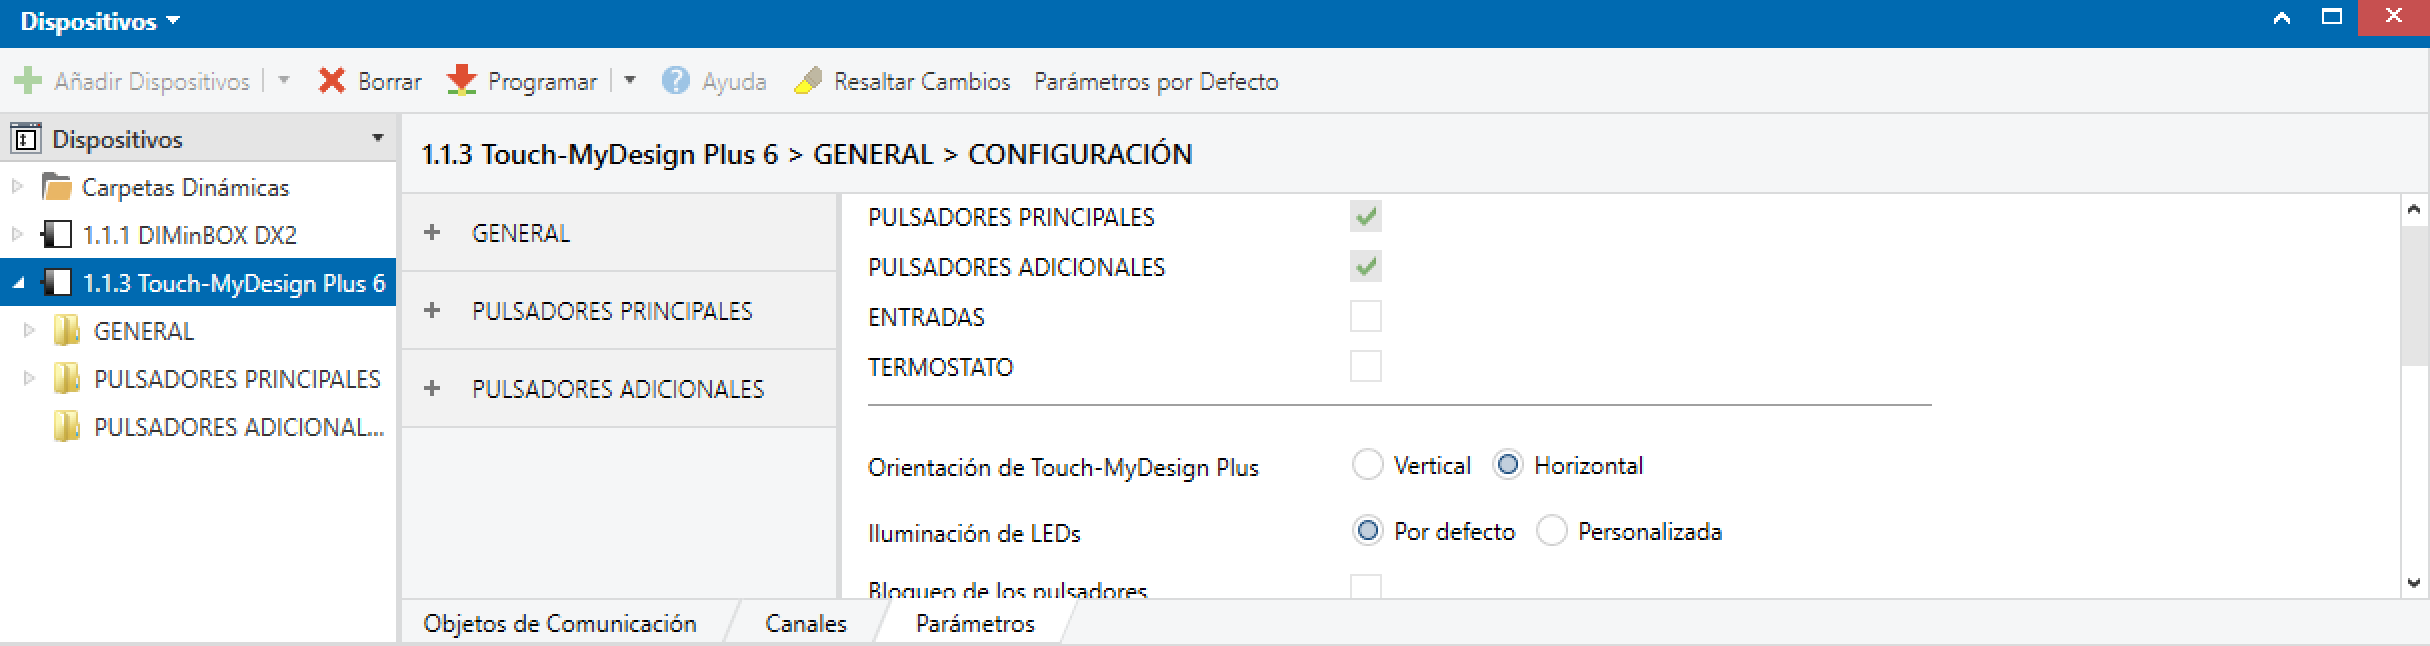
\includegraphics[width = 1.00\textwidth]{Imagenes/img6}
 		\captionof{figure}{\label{fig:IPN}Configurando parámetros del \textbf{Touch-MyDesign Plus 6} (I).} 
	\end{center} 
\end{figure}

\begin{figure}[H]
	\begin{center}
	 		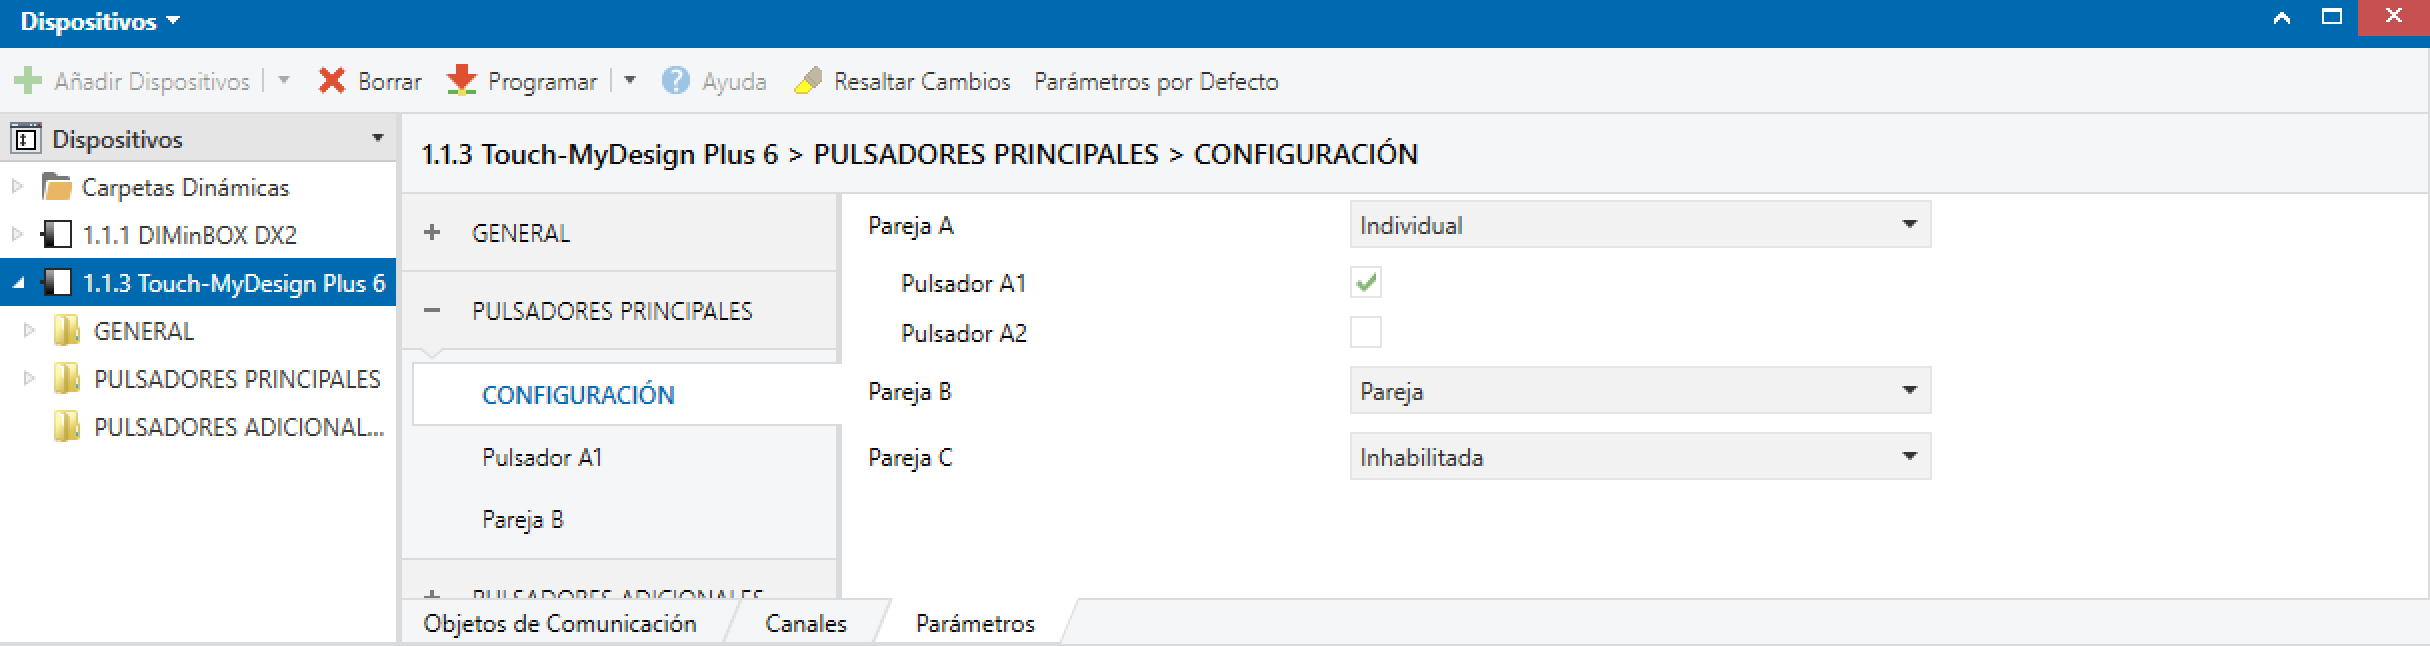
\includegraphics[width = 1.00\textwidth]{Imagenes/img7}
 		\captionof{figure}{\label{fig:IPN}Configurando parámetros del \textbf{Touch-MyDesign Plus 6} (II).} 
	\end{center} 
\end{figure}

\begin{figure}[H]
	\begin{center}
	 		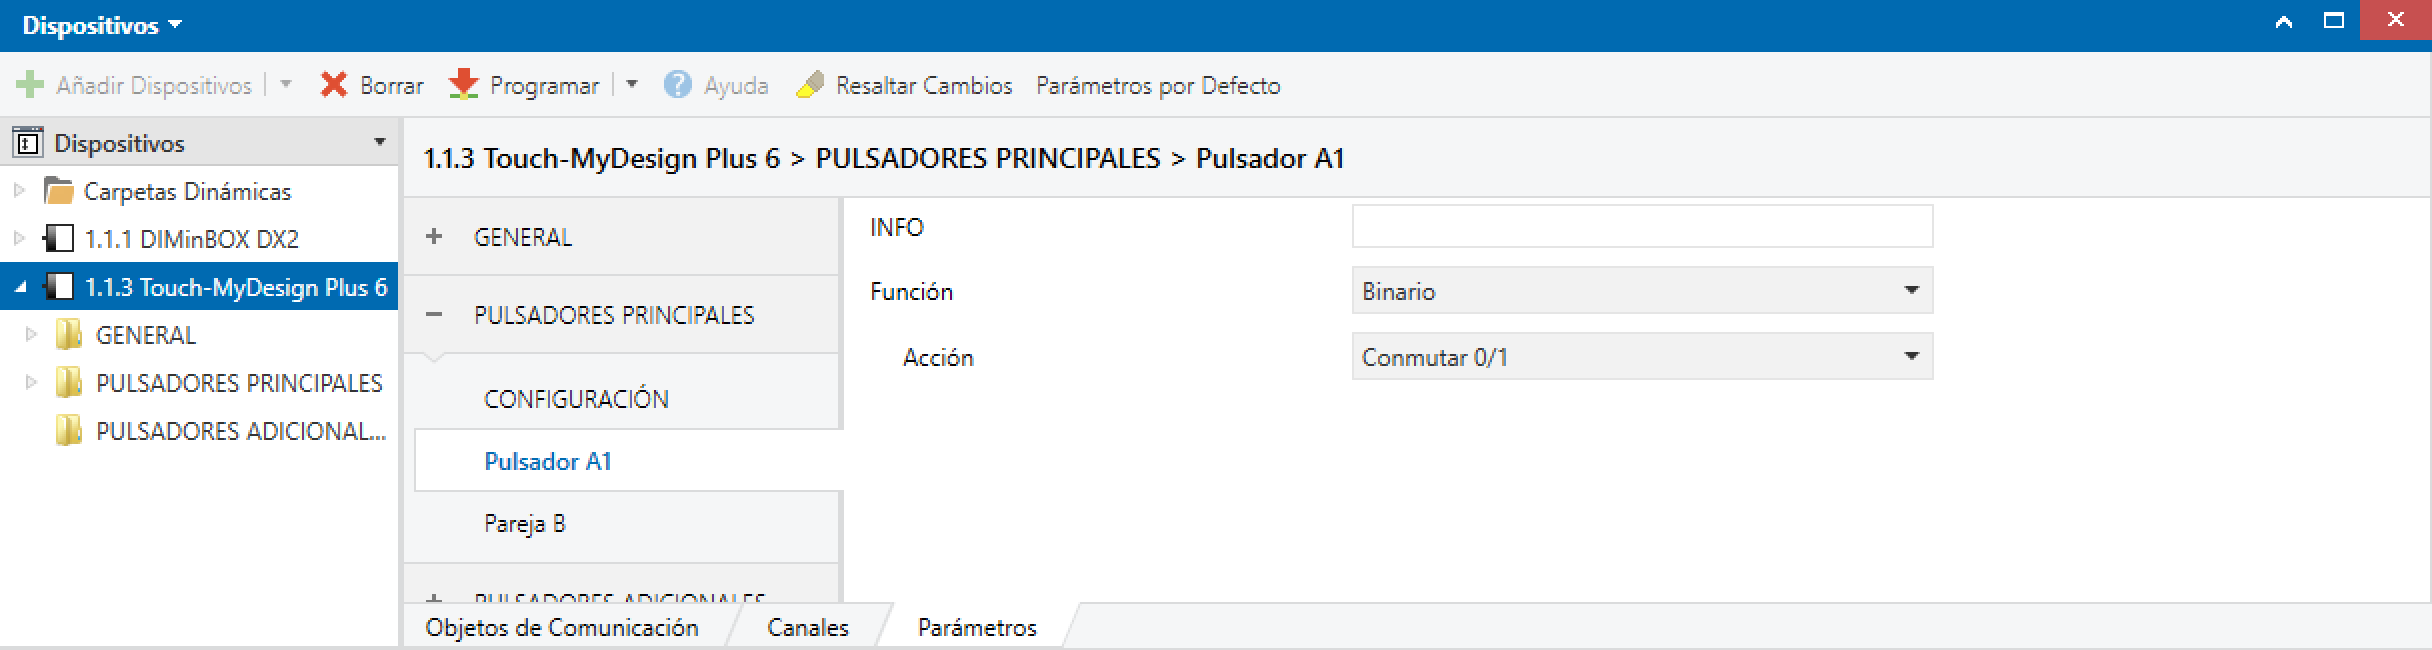
\includegraphics[width = 1.00\textwidth]{Imagenes/img8}
 		\captionof{figure}{\label{fig:IPN}Configurando parámetros del \textbf{Touch-MyDesign Plus 6} (III).} 
	\end{center} 
\end{figure}

\begin{figure}[H]
	\begin{center}
	 		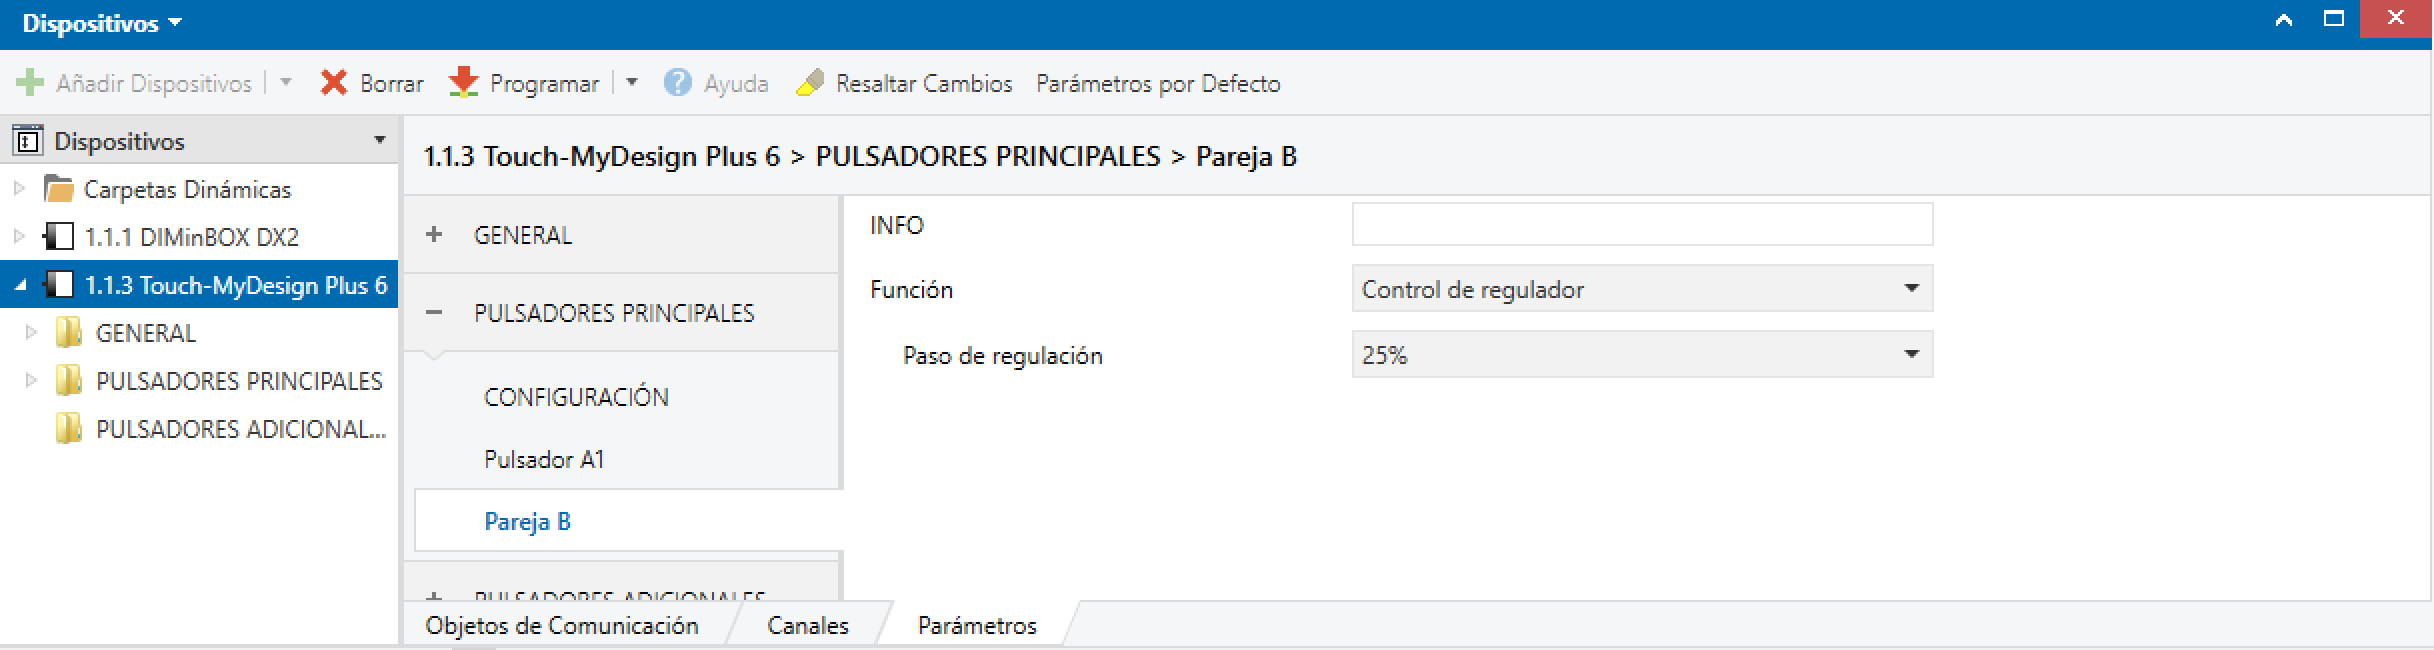
\includegraphics[width = 1.00\textwidth]{Imagenes/img9}
 		\captionof{figure}{\label{fig:IPN}Configurando parámetros del \textbf{Touch-MyDesign Plus 6} (IV).} 
	\end{center} 
\end{figure}

Pasamos ahora a definir las direcciones de grupo donde incluiremos los objetos de comunicación necesarios. Disponemos del grupo principal llamado \textbf{iluminación}, el cual contiene al grupo intermedio \textbf{Salón} del que a su vez cuelgan las direcciones de grupo \textbf{OnOff\_Luz\_Techo} y \textbf{Regulación}. \\

\begin{figure}[H]
	\begin{center}
	 		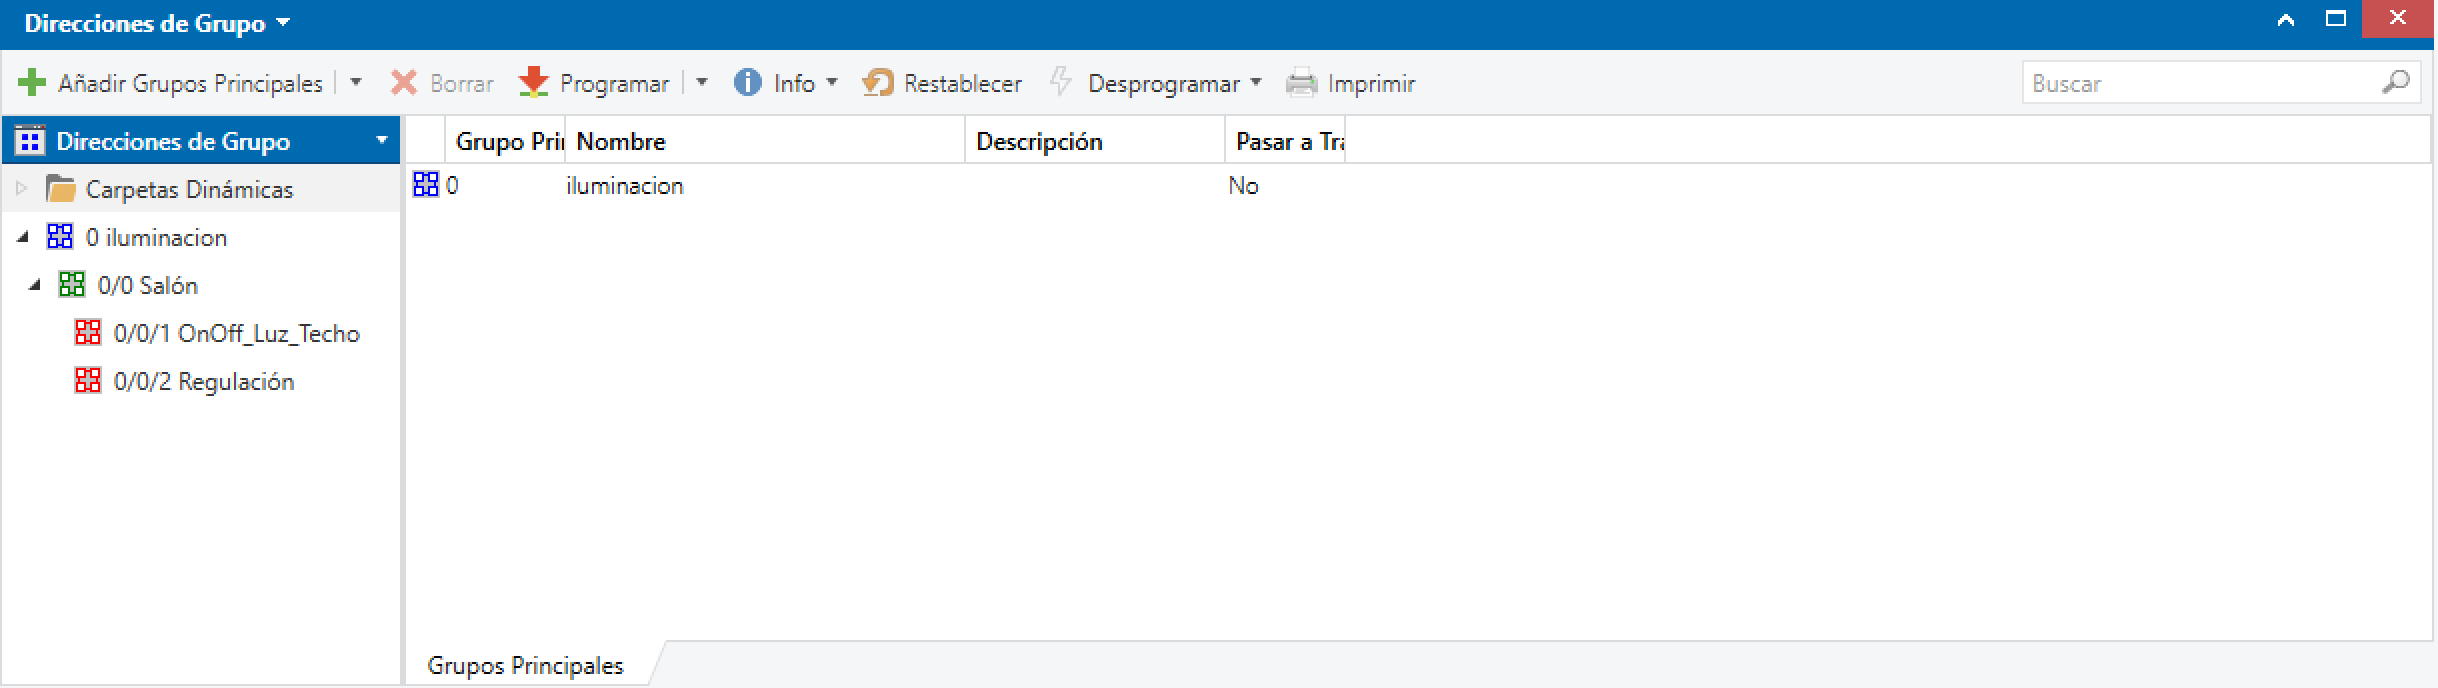
\includegraphics[width = 1.00\textwidth]{Imagenes/img10}
 		\captionof{figure}{\label{fig:IPN}Estableciendo las direcciones de grupo.} 
	\end{center} 
\end{figure}

A la dirección de grupo \textbf{OnOff\_Luz\_Techo} le añadiremos los objetos de comunicación ``On/Off'' del dispositivo \textbf{DIMinBOX DX2} de la salida \textbf{C1} y el objeto de comunicación ``Control binario'' del pulsador principal \textbf{A1} perteneciente al dispositivo  \textbf{Touch-MyDesign Plus 6}. \\

\begin{figure}[H]
	\begin{center}
	 		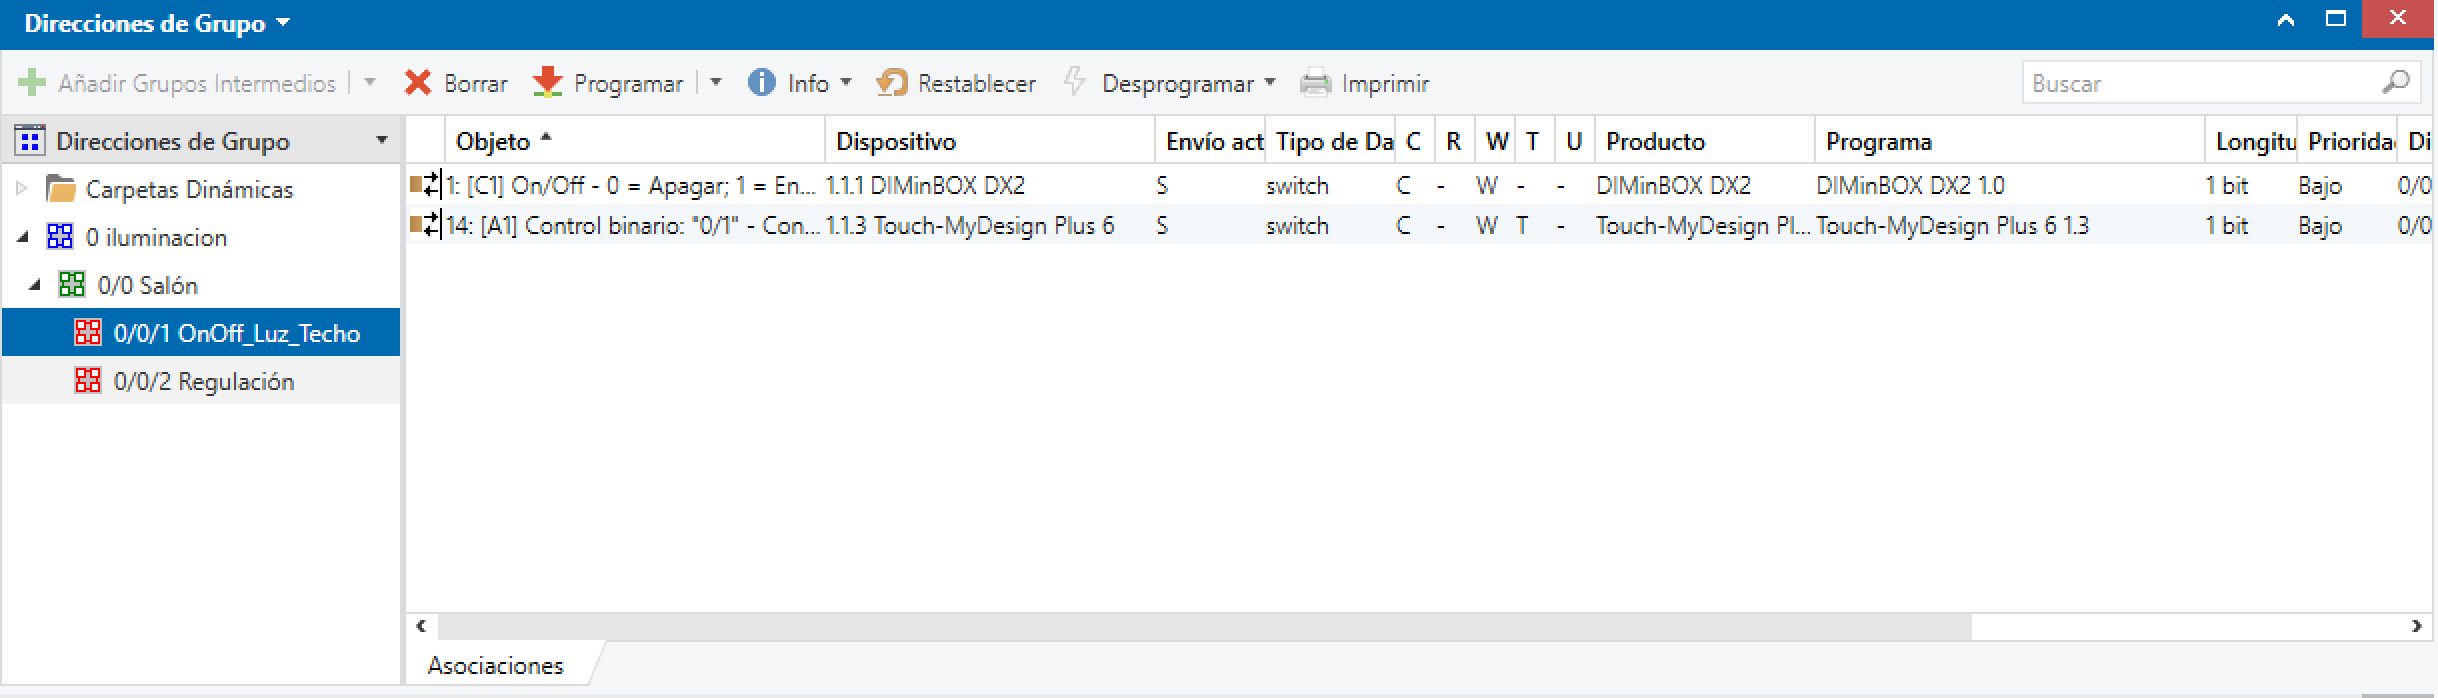
\includegraphics[width = 1.00\textwidth]{Imagenes/img11}
 		\captionof{figure}{\label{fig:IPN}Añadiendo objetos de comunicación a la dirección de grupo \textbf{OnOff\_Luz\_Techo}.} 
	\end{center} 
\end{figure}

\begin{figure}[H]
	\begin{center}
	 		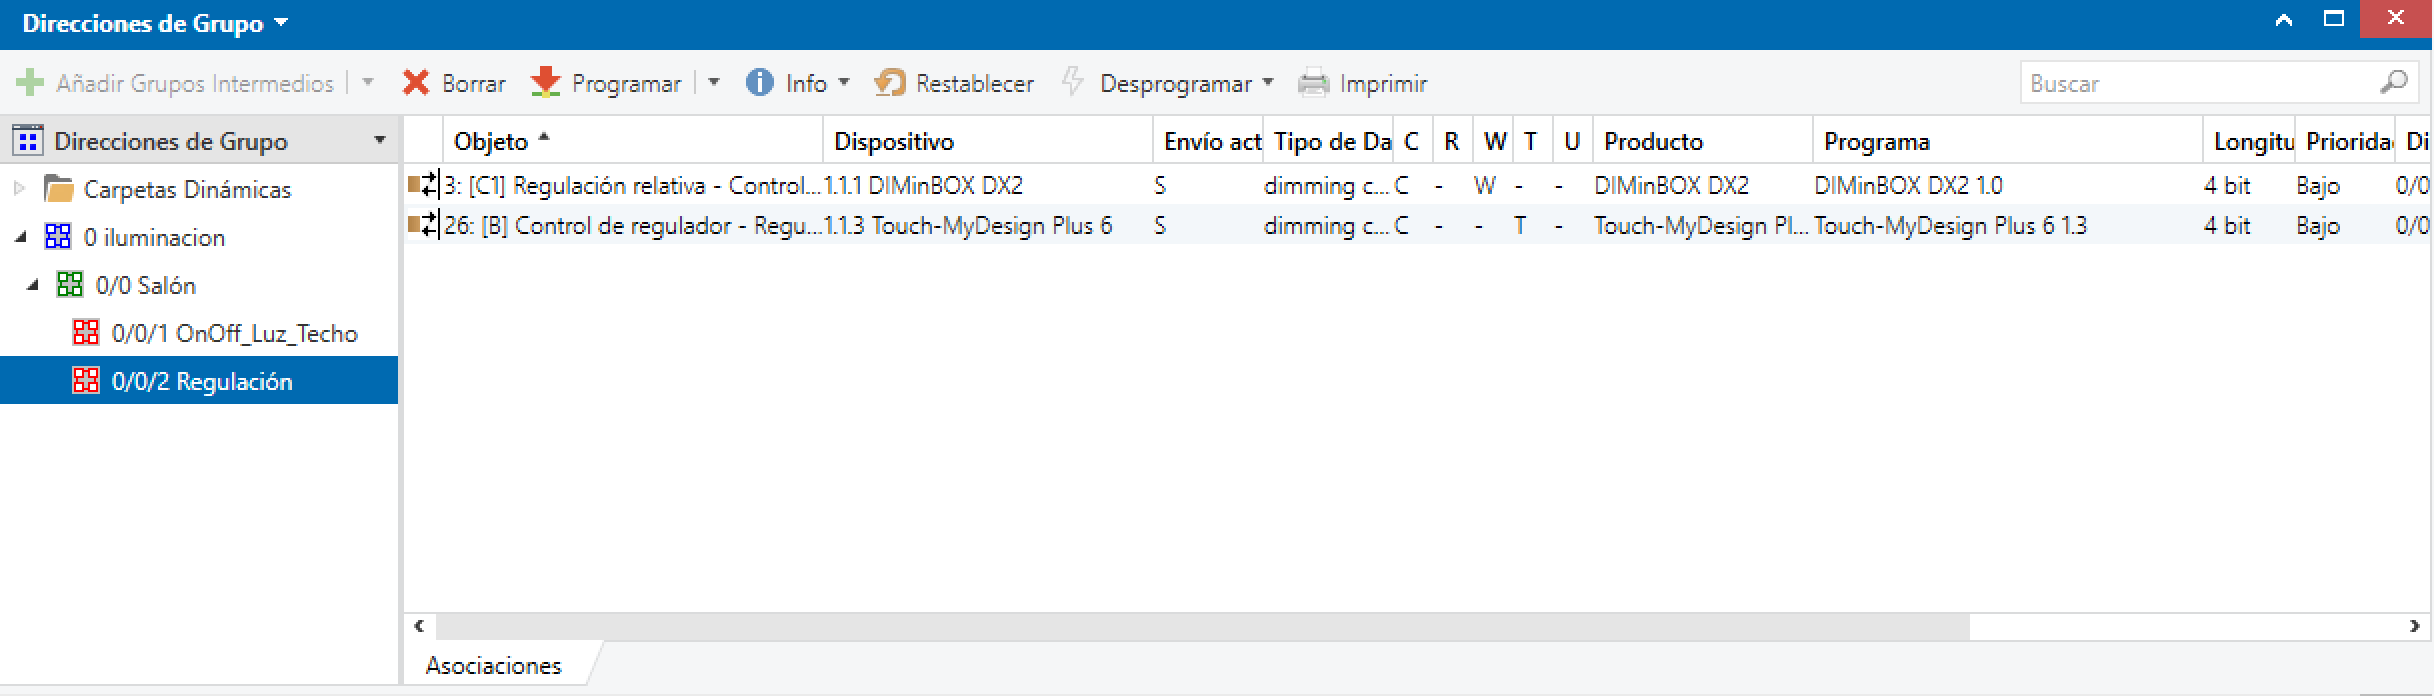
\includegraphics[width = 1.00\textwidth]{Imagenes/img12}
 		\captionof{figure}{\label{fig:IPN}Añadiendo objetos de comunicación a la dirección de grupo \textbf{Regulación}.} 
	\end{center} 
\end{figure}

Terminada esta configuración, el sitema queda totalmente configurado para ser programado y lanzado en el entorno de pruebas KNX para comprobar su correcto funcionamiento como se pudo corrobar en el laboratorio de prácticas. \\


\section{Práctica 2. Control de presencia.} 
Para este segundo supuesto se configurará el sistema KNX para realizar un control de presencia. La finalidad del mismo es la de activar la iluminación cuando detecte presencia en la habitación y desactivarla cuando no detecte presencia alguna pasado un tiempo parametizable. \\

Vamos a utilizar la configuración empleada en la práctica anterior (mismos dispositivos, direcciones de grupo, parámetros, etc.) a la que le haremos una serie de modificaciones para adapatarla al supuesto actual. Lo primero que vamos a hacer es configurar los parámetros del \textbf{DIMinBOX DX2} de modo que a una de sus dos entradas (\textbf{E1} y \textbf{E2}) le habilitemos el detector de movimiento, en este caso para la entrada 2 (\textbf{E2}). Configuraremos dicha entrada para que se produzca el envío de luminosidad periódicamente cada 4 segundos por el canal 1. En dicho canal estableceremos un tiempo de 10 segundos para la duración de la detección, asignando un retardo de reinicio de 1 segundo. Le estableceremos un umbral del 60\%, por lo que cuando el valor de luminosidad baje de ese umbral y detecte presencia se activarán las luces, por el contrario si el umbral está por encima de ese valor no activará las luces al igual que si no detecta presencia alguna en la habitación pasados los 10 segundos de la detección establecidos anteriormente. En las siguientes imagenes se pueden ver dichos valores de la parametrización. \\

\begin{figure}[H]
	\begin{center}
	 		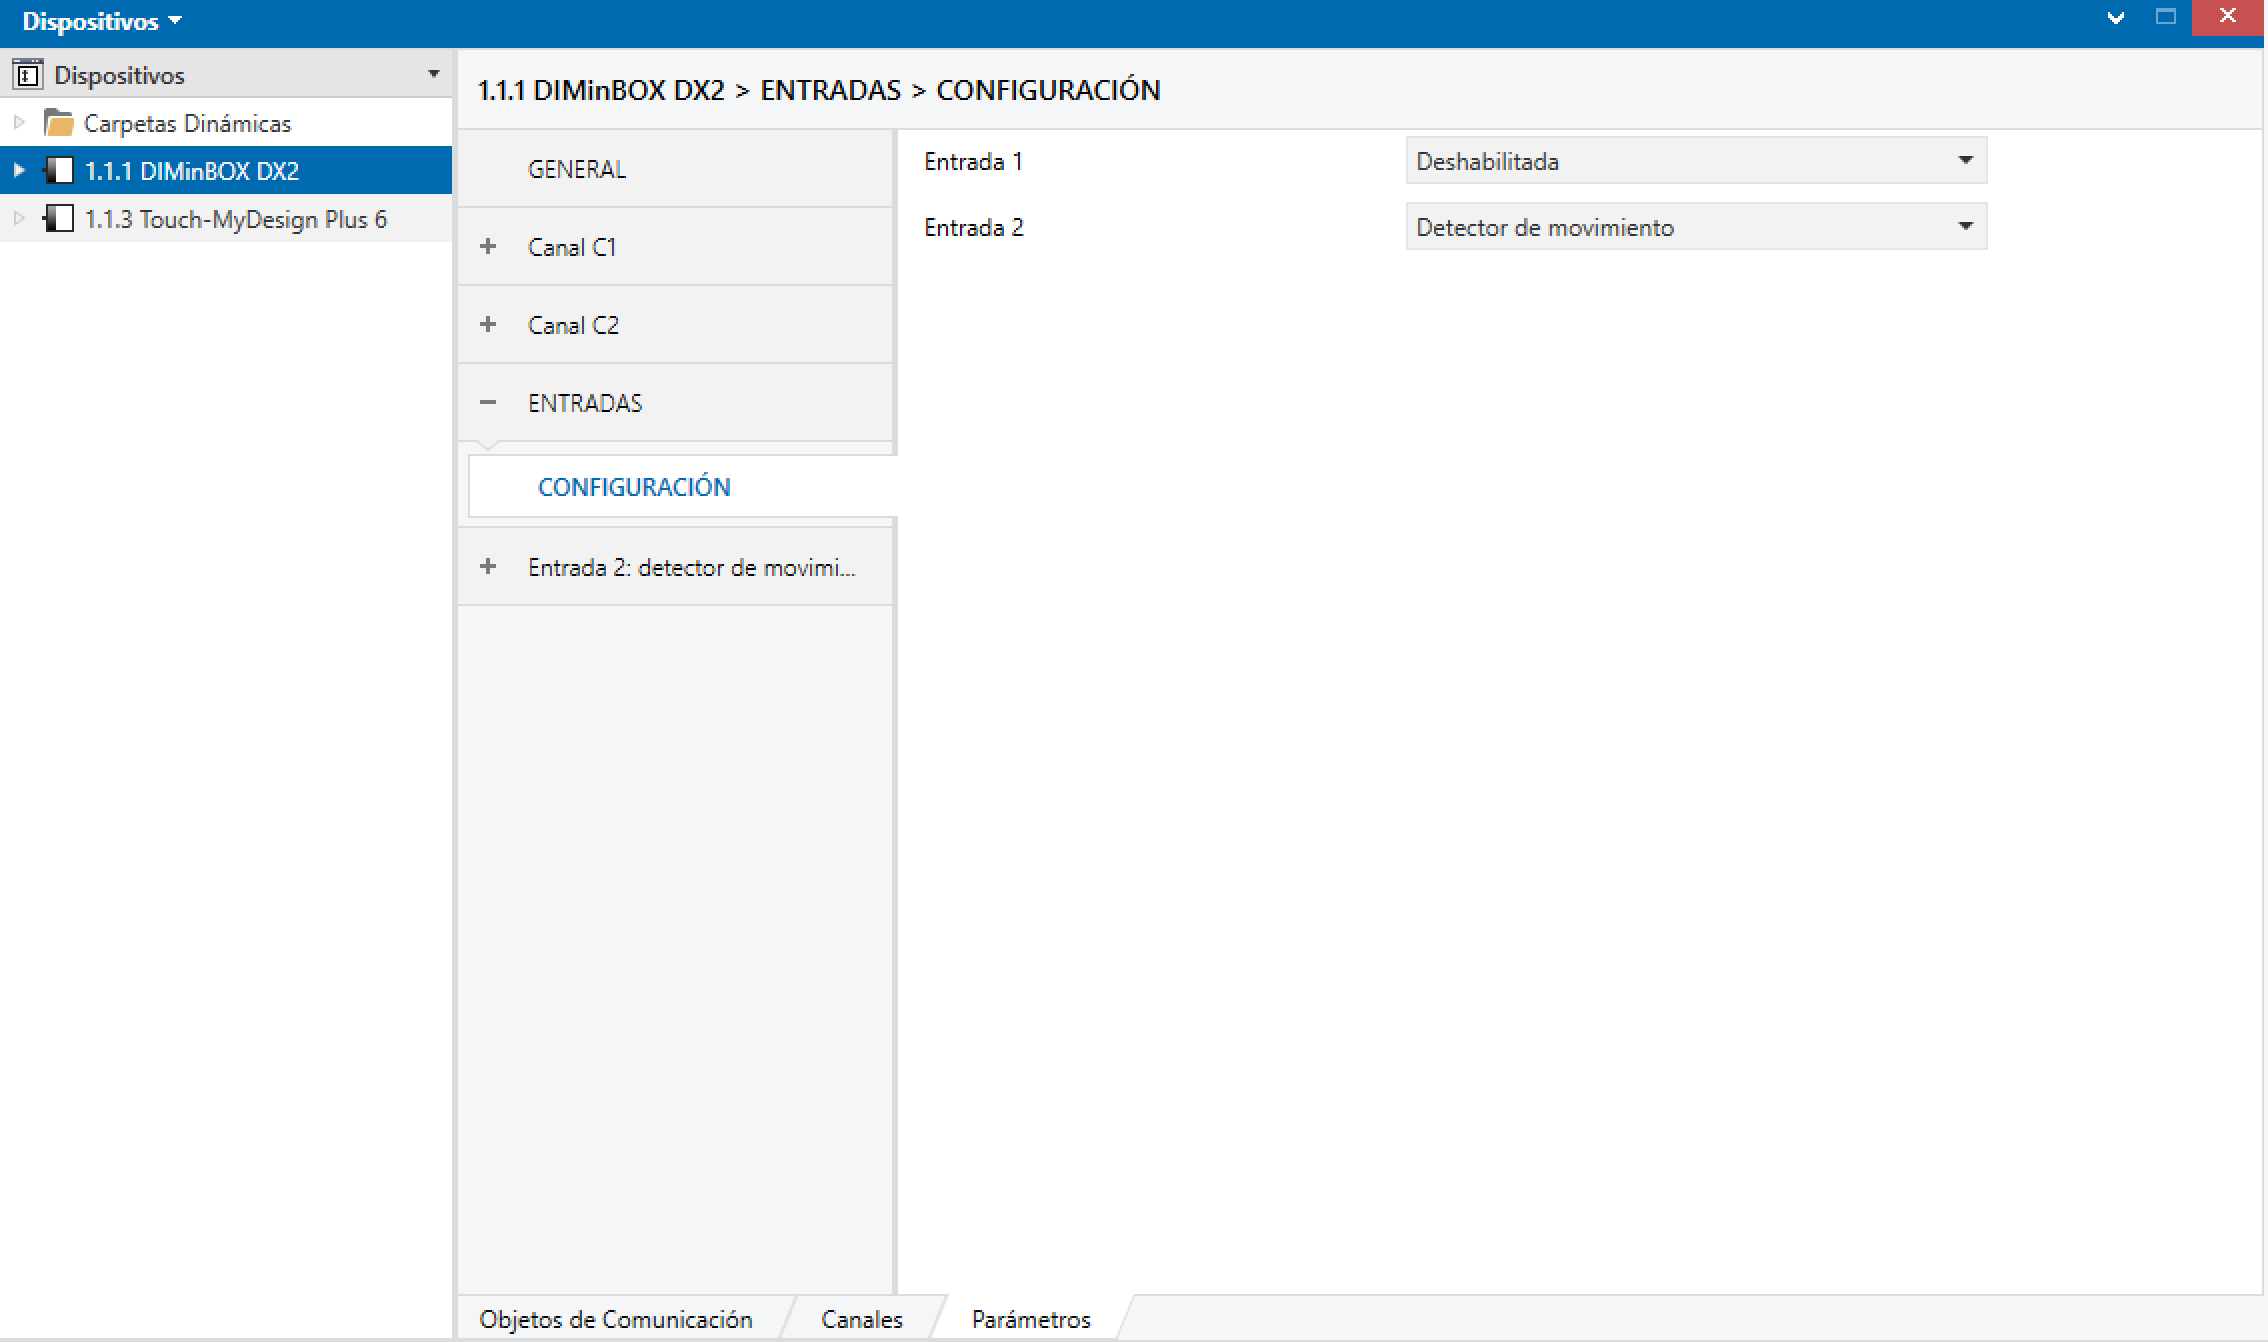
\includegraphics[width = 1.00\textwidth]{Imagenes/img13}
 		\captionof{figure}{\label{fig:IPN}Configurando parámetros del \textbf{DIMinBOX DX2} (I).} 
	\end{center} 
\end{figure}

\begin{figure}[H]
	\begin{center}
	 		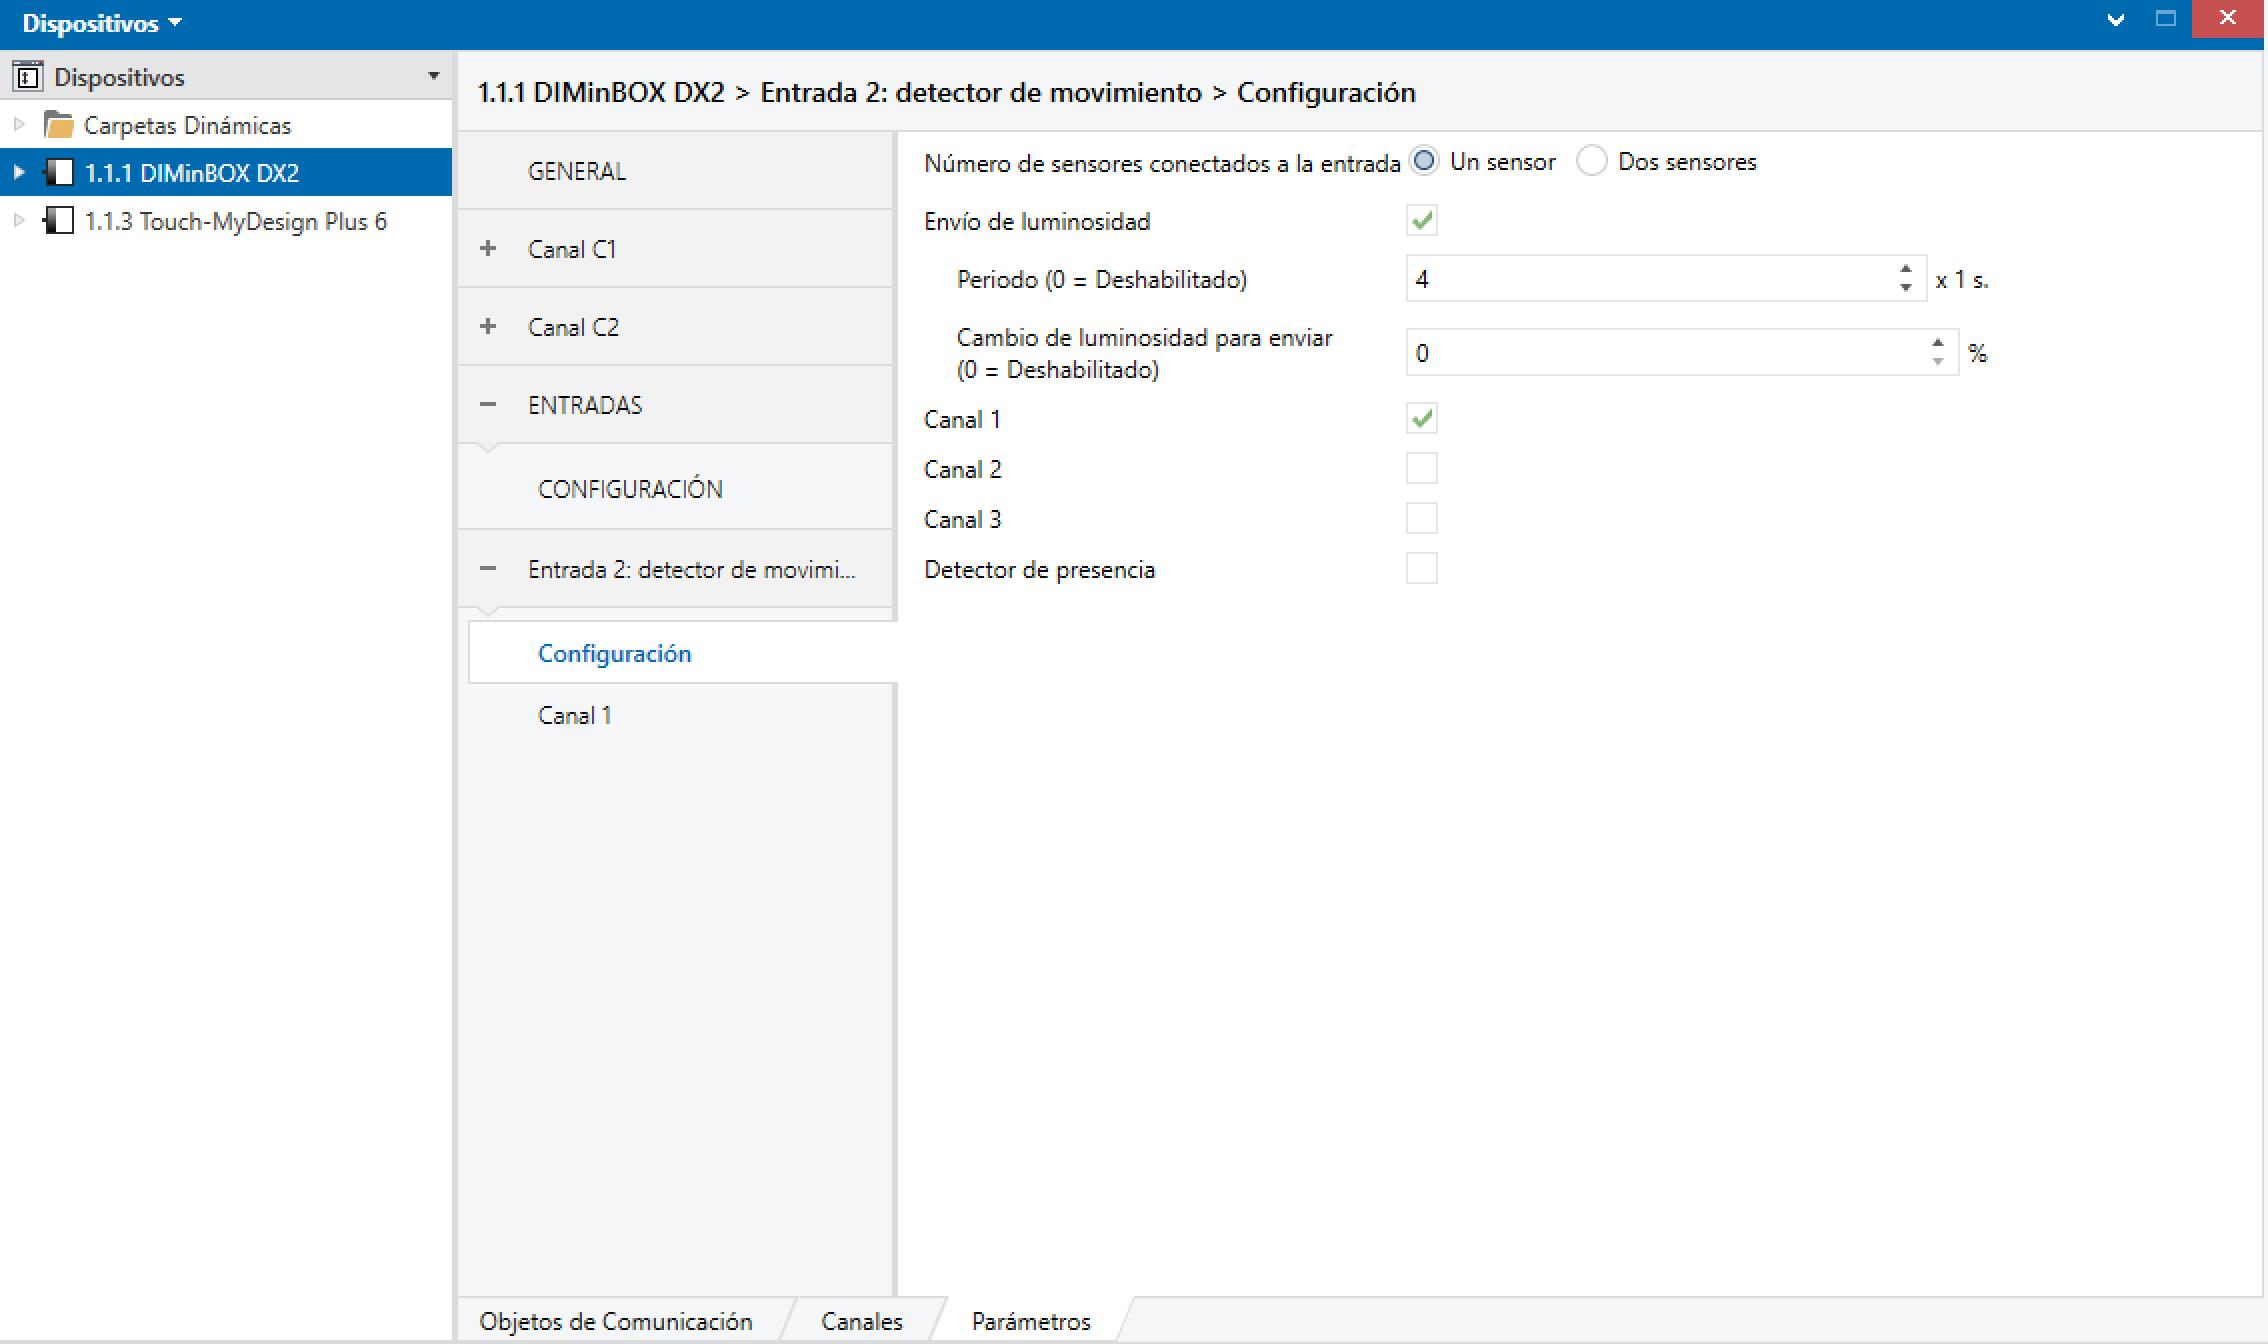
\includegraphics[width = 1.00\textwidth]{Imagenes/img14}
 		\captionof{figure}{\label{fig:IPN}Configurando parámetros del \textbf{DIMinBOX DX2} (II).} 
	\end{center} 
\end{figure}

\begin{figure}[H]
	\begin{center}
	 		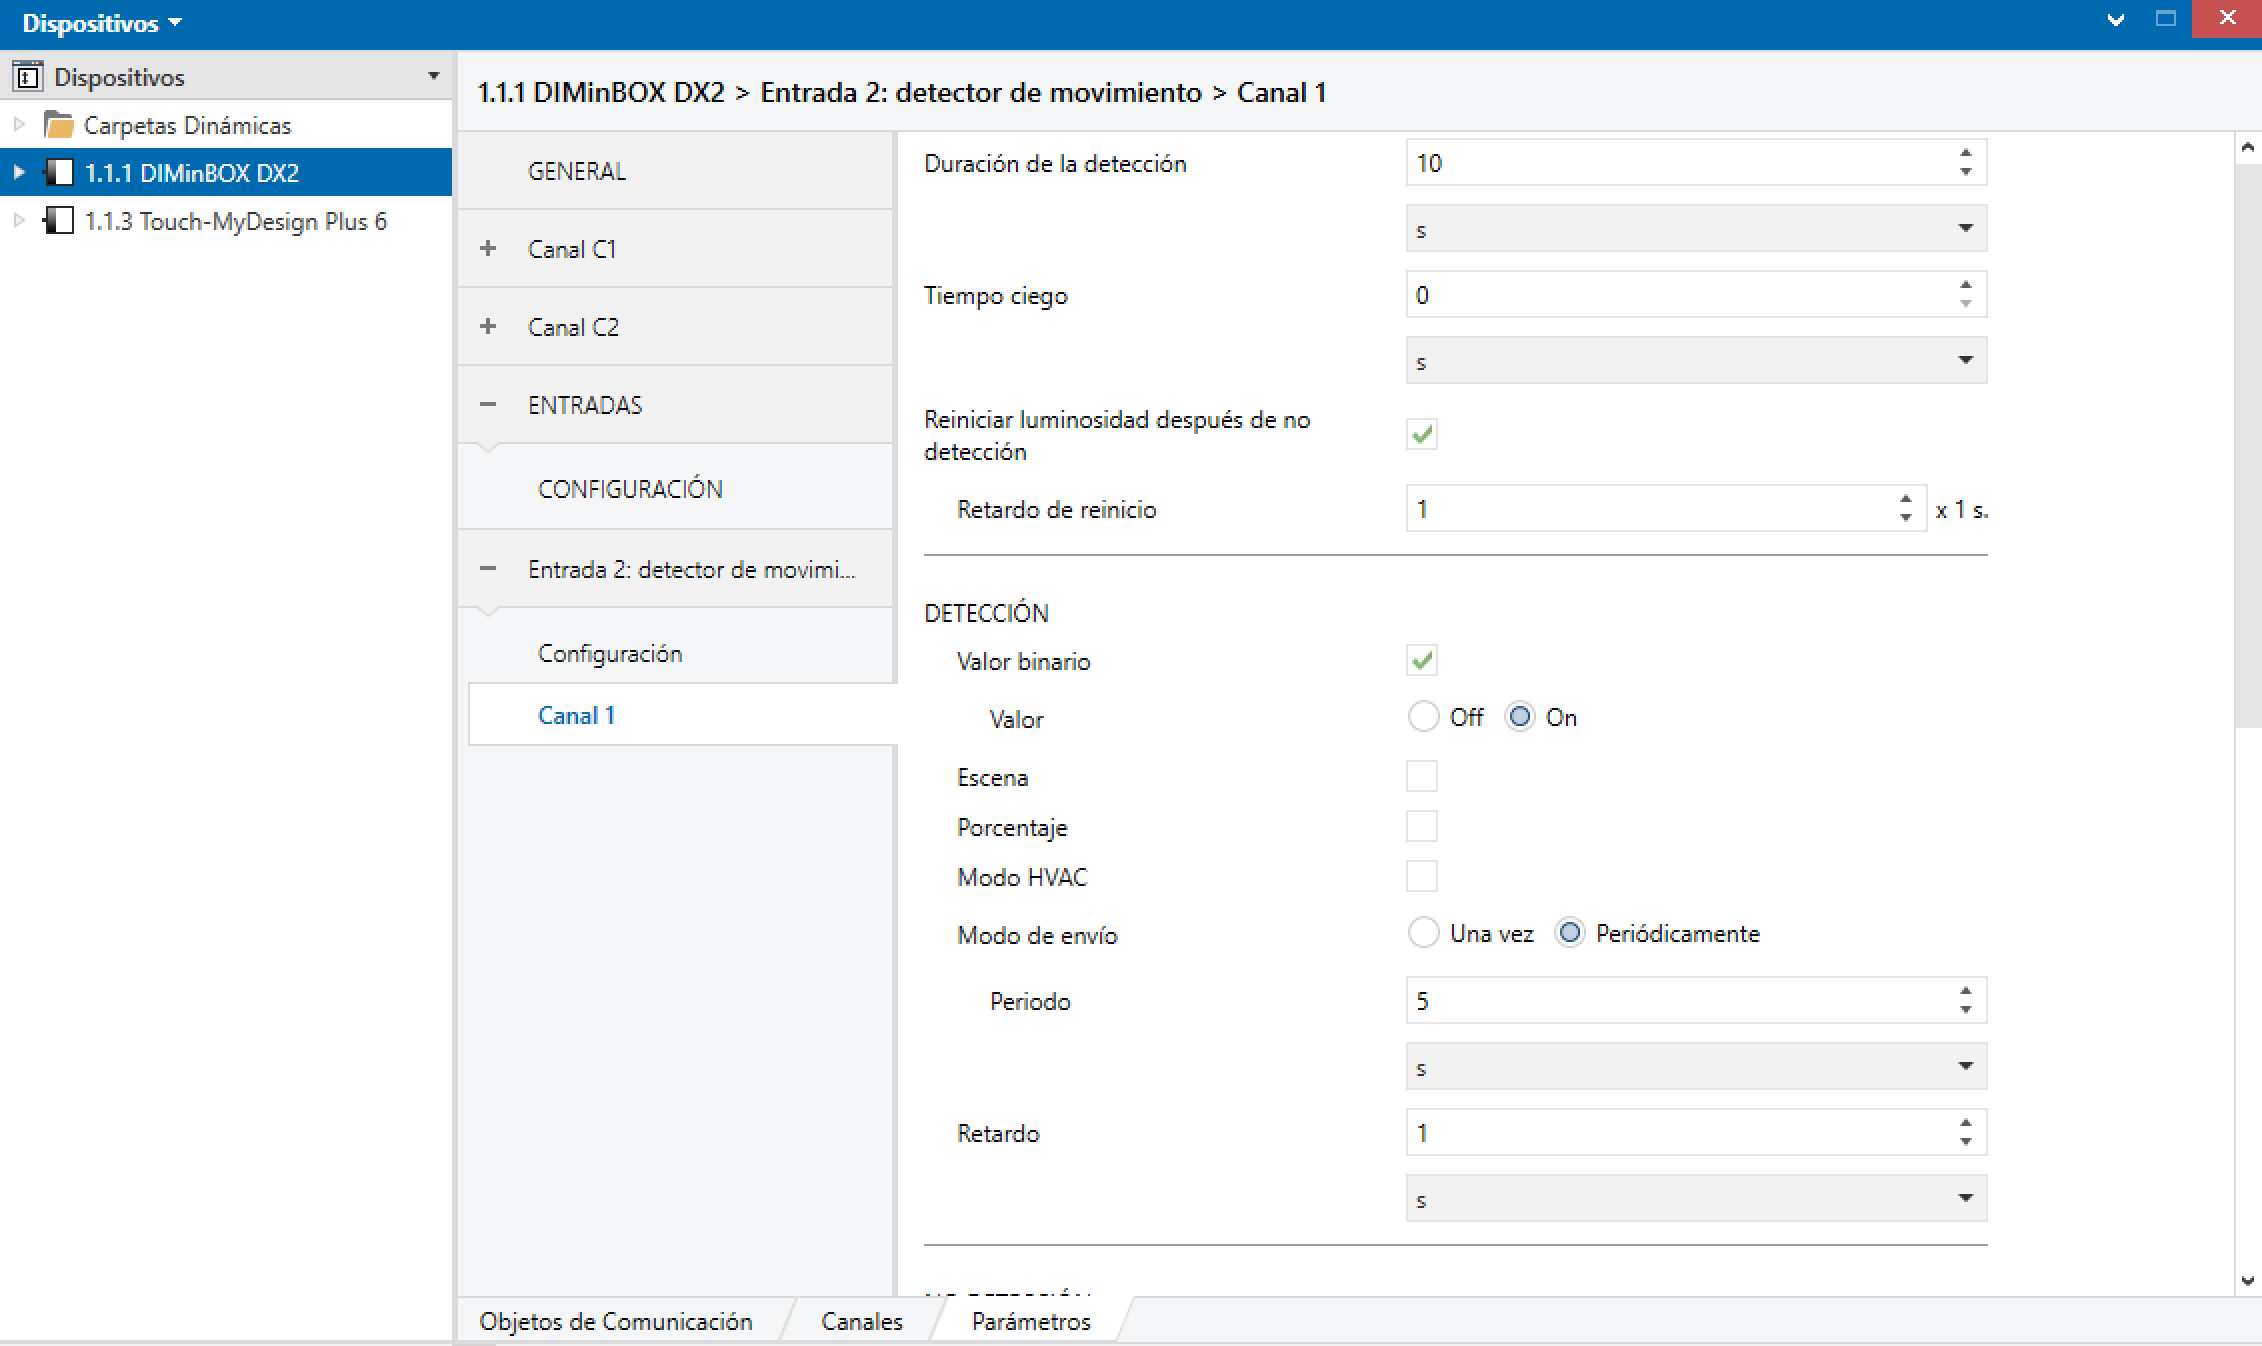
\includegraphics[width = 1.00\textwidth]{Imagenes/img15}
 		\captionof{figure}{\label{fig:IPN}Configurando parámetros del \textbf{DIMinBOX DX2} (III).} 
	\end{center} 
\end{figure}

\begin{figure}[H]
	\begin{center}
	 		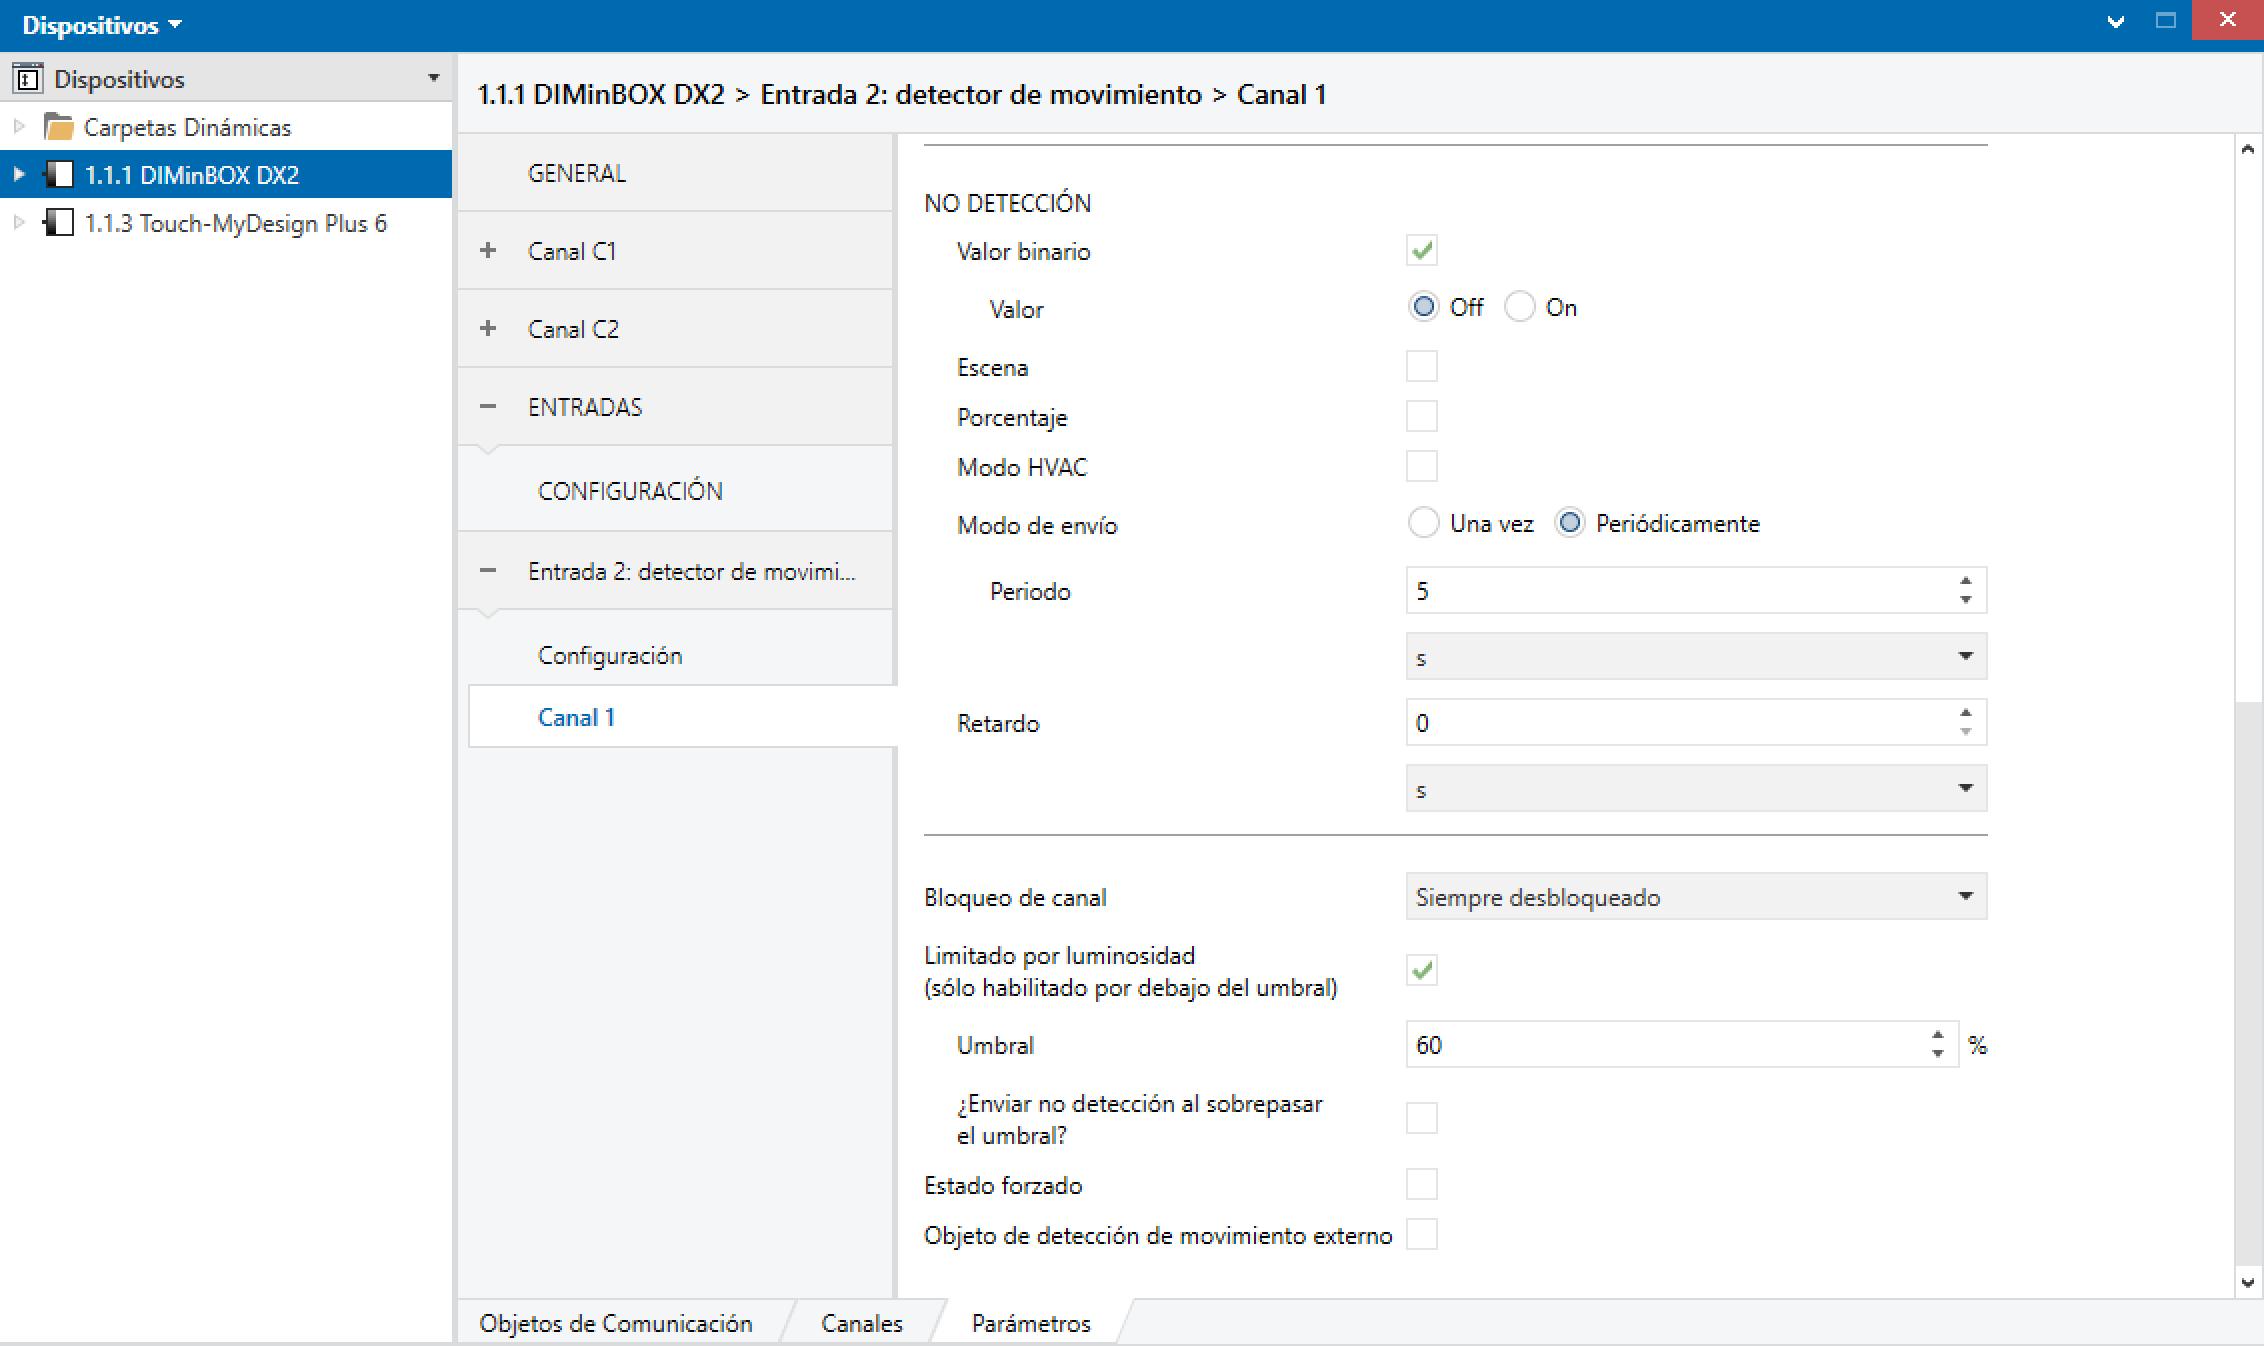
\includegraphics[width = 1.00\textwidth]{Imagenes/img16}
 		\captionof{figure}{\label{fig:IPN}Configurando parámetros del \textbf{DIMinBOX DX2} (IV).} 
	\end{center} 
\end{figure}

La entrada configurada \textbf{E2} dispone de los siguientes objetos de comunicación. \\

\begin{figure}[H]
	\begin{center}
	 		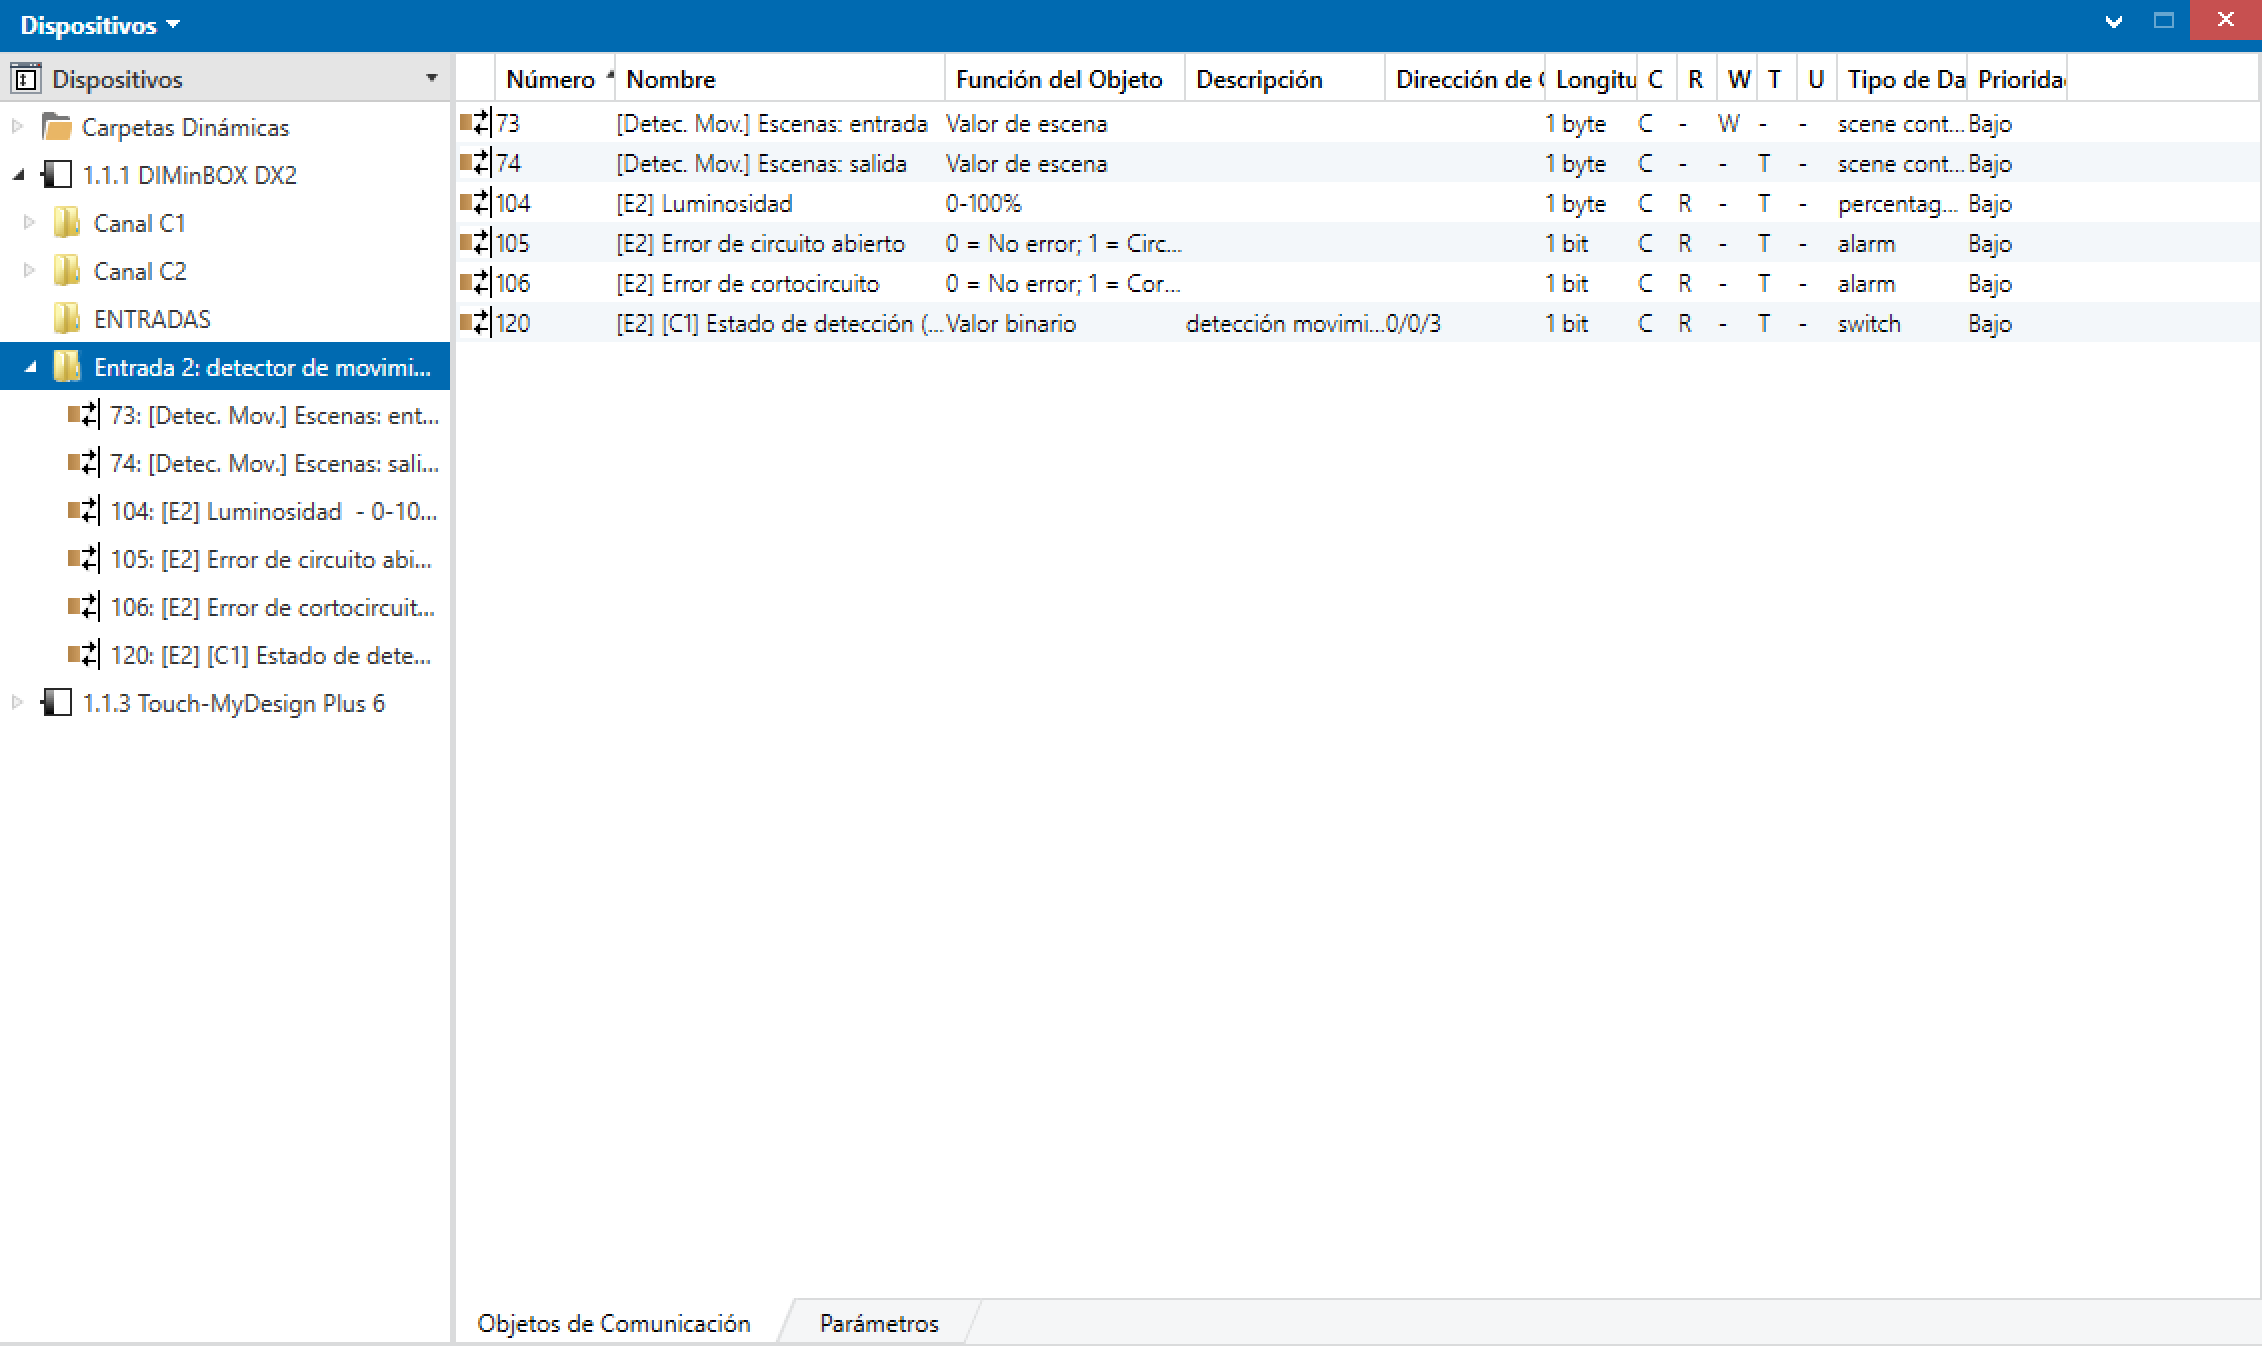
\includegraphics[width = 1.00\textwidth]{Imagenes/img17}
 		\captionof{figure}{\label{fig:IPN}Objetos de comunicación para la entrada \textbf{E2} del \textbf{DIMinBOX DX2}.} 
	\end{center} 
\end{figure}

Vamos ahora a definir una nueva dirección de grupo llamada \textbf{detección movimiento} donde añadiremos los correspondientes objetos de comunicación de la entrada \textbf{E2}. En dicha dirección de grupo solamente incluiremos objetos de comunicación del módulo \textbf{DIMinBOX DX2} ya que no se necesita de ninguno otro más para realizar este supuesto. Agregaremos los objetos ``On/Off'' de cada una de las salidas \textbf{C1} y \textbf{C2} para que se enciende o apaguen las lámparas led, así como el objeto ``Estado de detección'' de la entrada \textbf{E2} y el canal 1 \textbf{C1} que se configuró previamente. \\

\begin{figure}[H]
	\begin{center}
	 		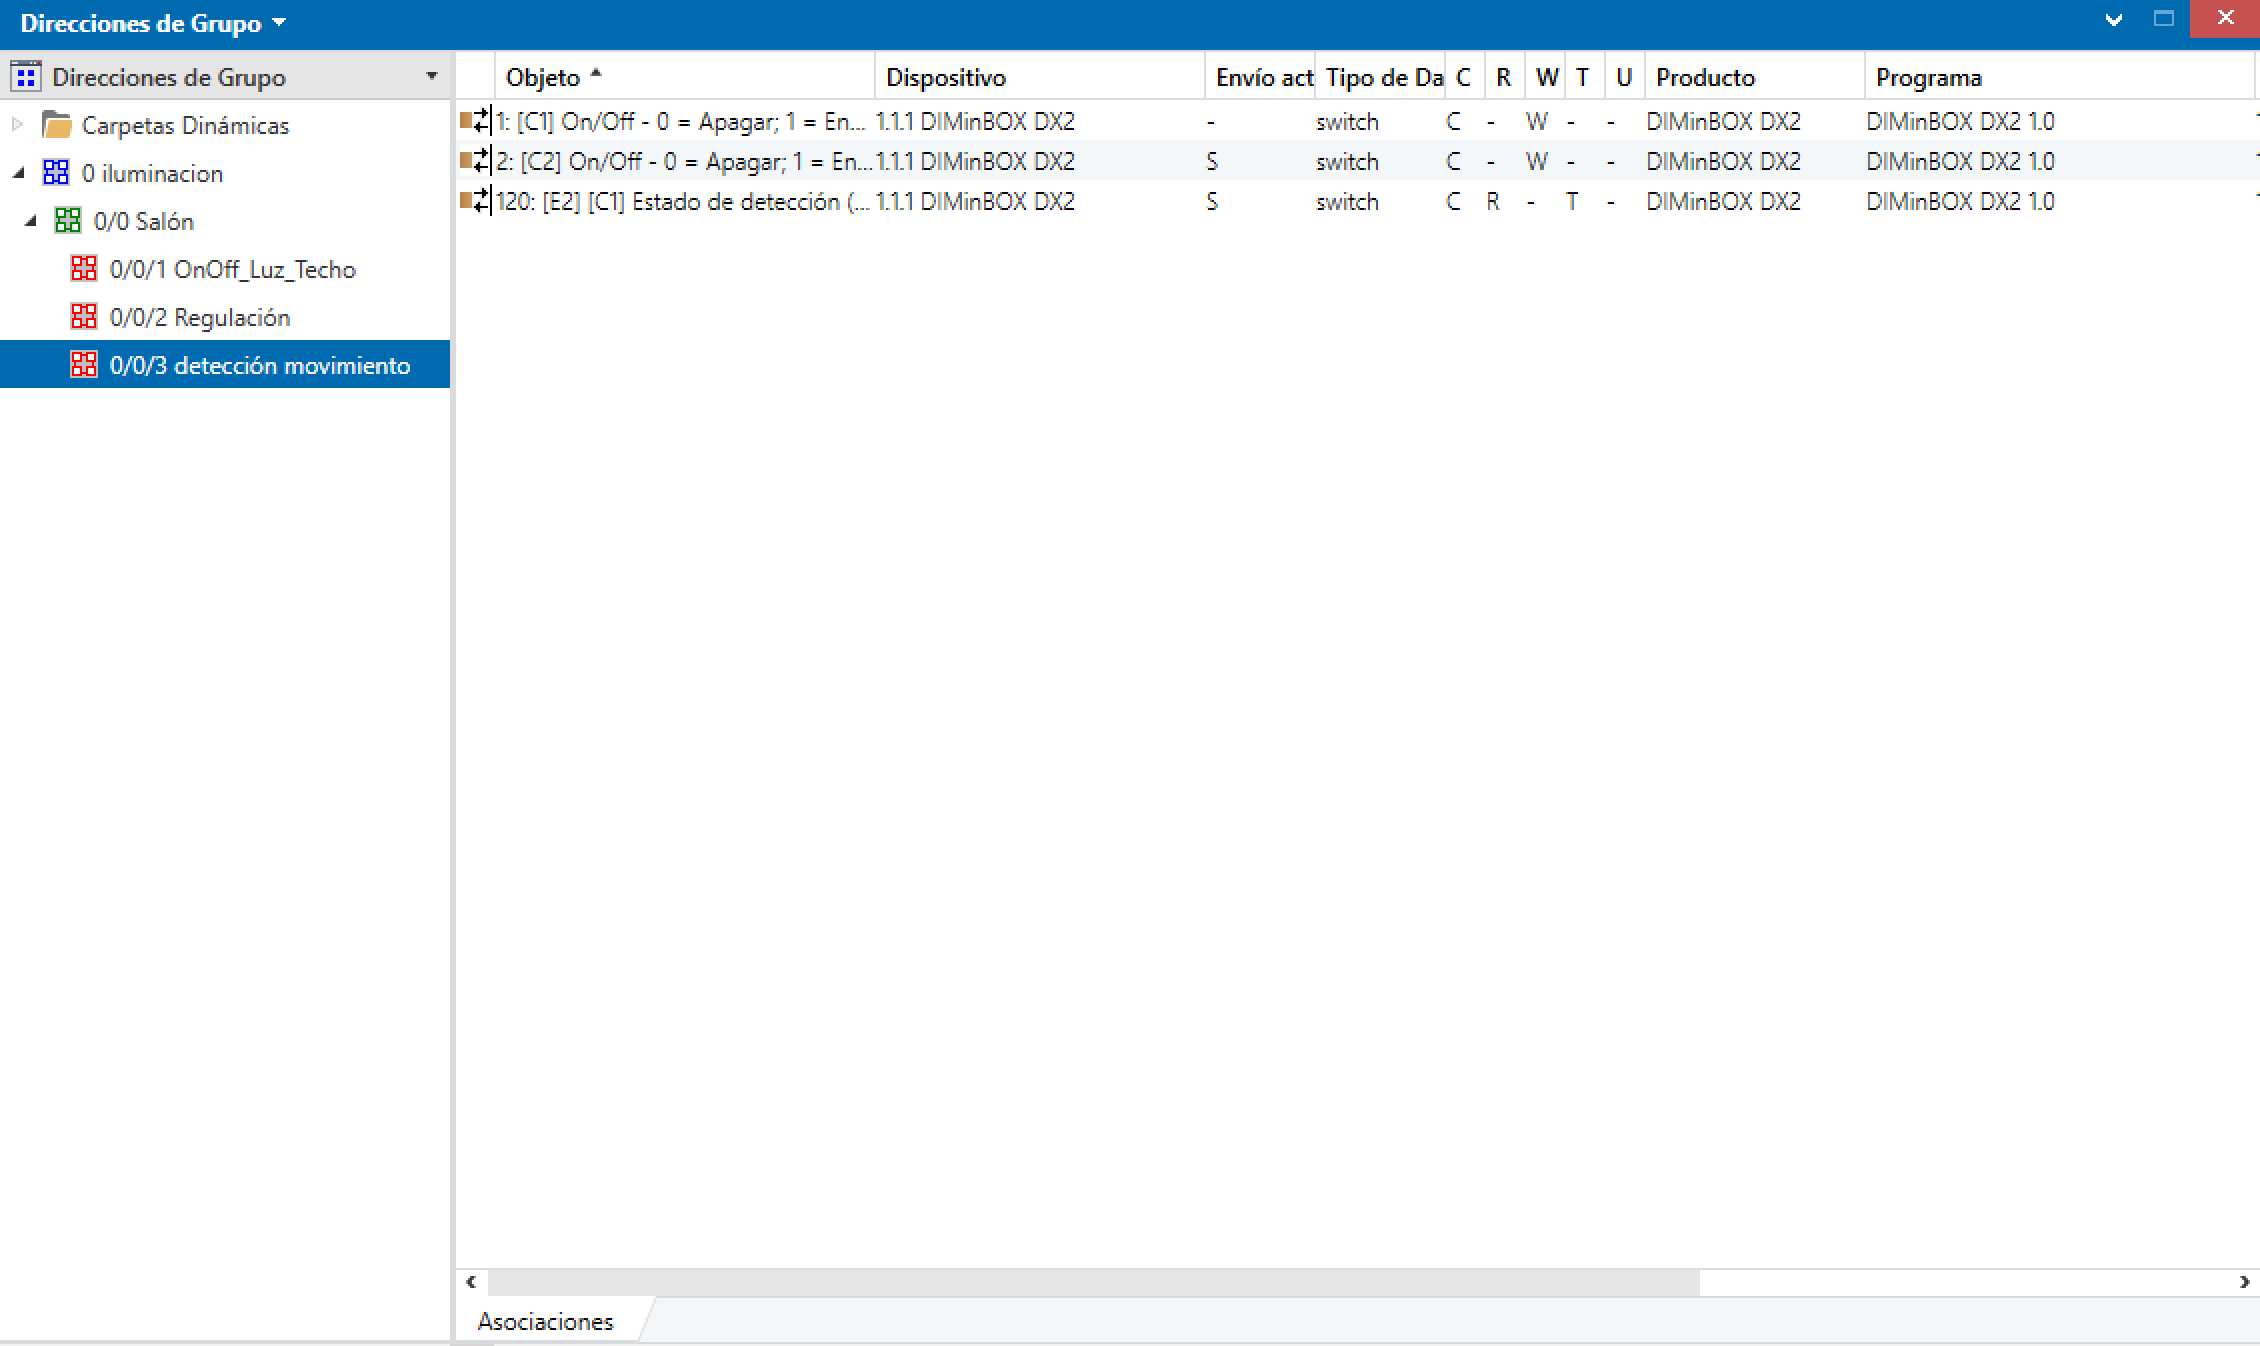
\includegraphics[width = 1.00\textwidth]{Imagenes/img18}
 		\captionof{figure}{\label{fig:IPN}Añadiendo objeto de comunicación a la dirección de grupo  \textbf{detección movimiento}.} 
	\end{center} 
\end{figure}

Con el sistema configurado y preparado solo queda programarlo para ser lanzado. Cabe destacar que en este caso al tomar como base el proyecto de la práctica anterior no es necesario realizar una programación de todo ya que para probar este supuesto sólo nos basamos en la dirección de grupo \textbf{detección movimiento}, por lo que podemos hacer una programación parcial de la misma como hicimos en el laboratorio de prácticas para comprobar su correcto funcionamiento.\\


\section{Práctica 3. Control de temperatura.} 
Para esta práctica se configurará el sistema KNX para realizar un control de temperatura. La finalidad de este supuesto es activar o desactivar un termostato en función de la temperatura que el sensor capte y de la que esté establecida como consigna. Esta práctica se hace en conjunto con la práctica de \textbf{Uso de un panel táctil} de manera que a través de dicho panel se podrá configurar la temperatura de consigna aumentándola o disminuyéndola en función de lo requerido. \\

Una vez creado el nuevo proyecto pasamos a agregar los dispositivos necesarios para la realización del mismo. Para este supuesto será necesario añadir los módulos \textbf{DIMinBOX DX2}, \textbf{MINiBOX 45} y \textbf{Z41 Pro} como se muestra en la imagen. \\

\begin{figure}[H]
	\begin{center}
	 		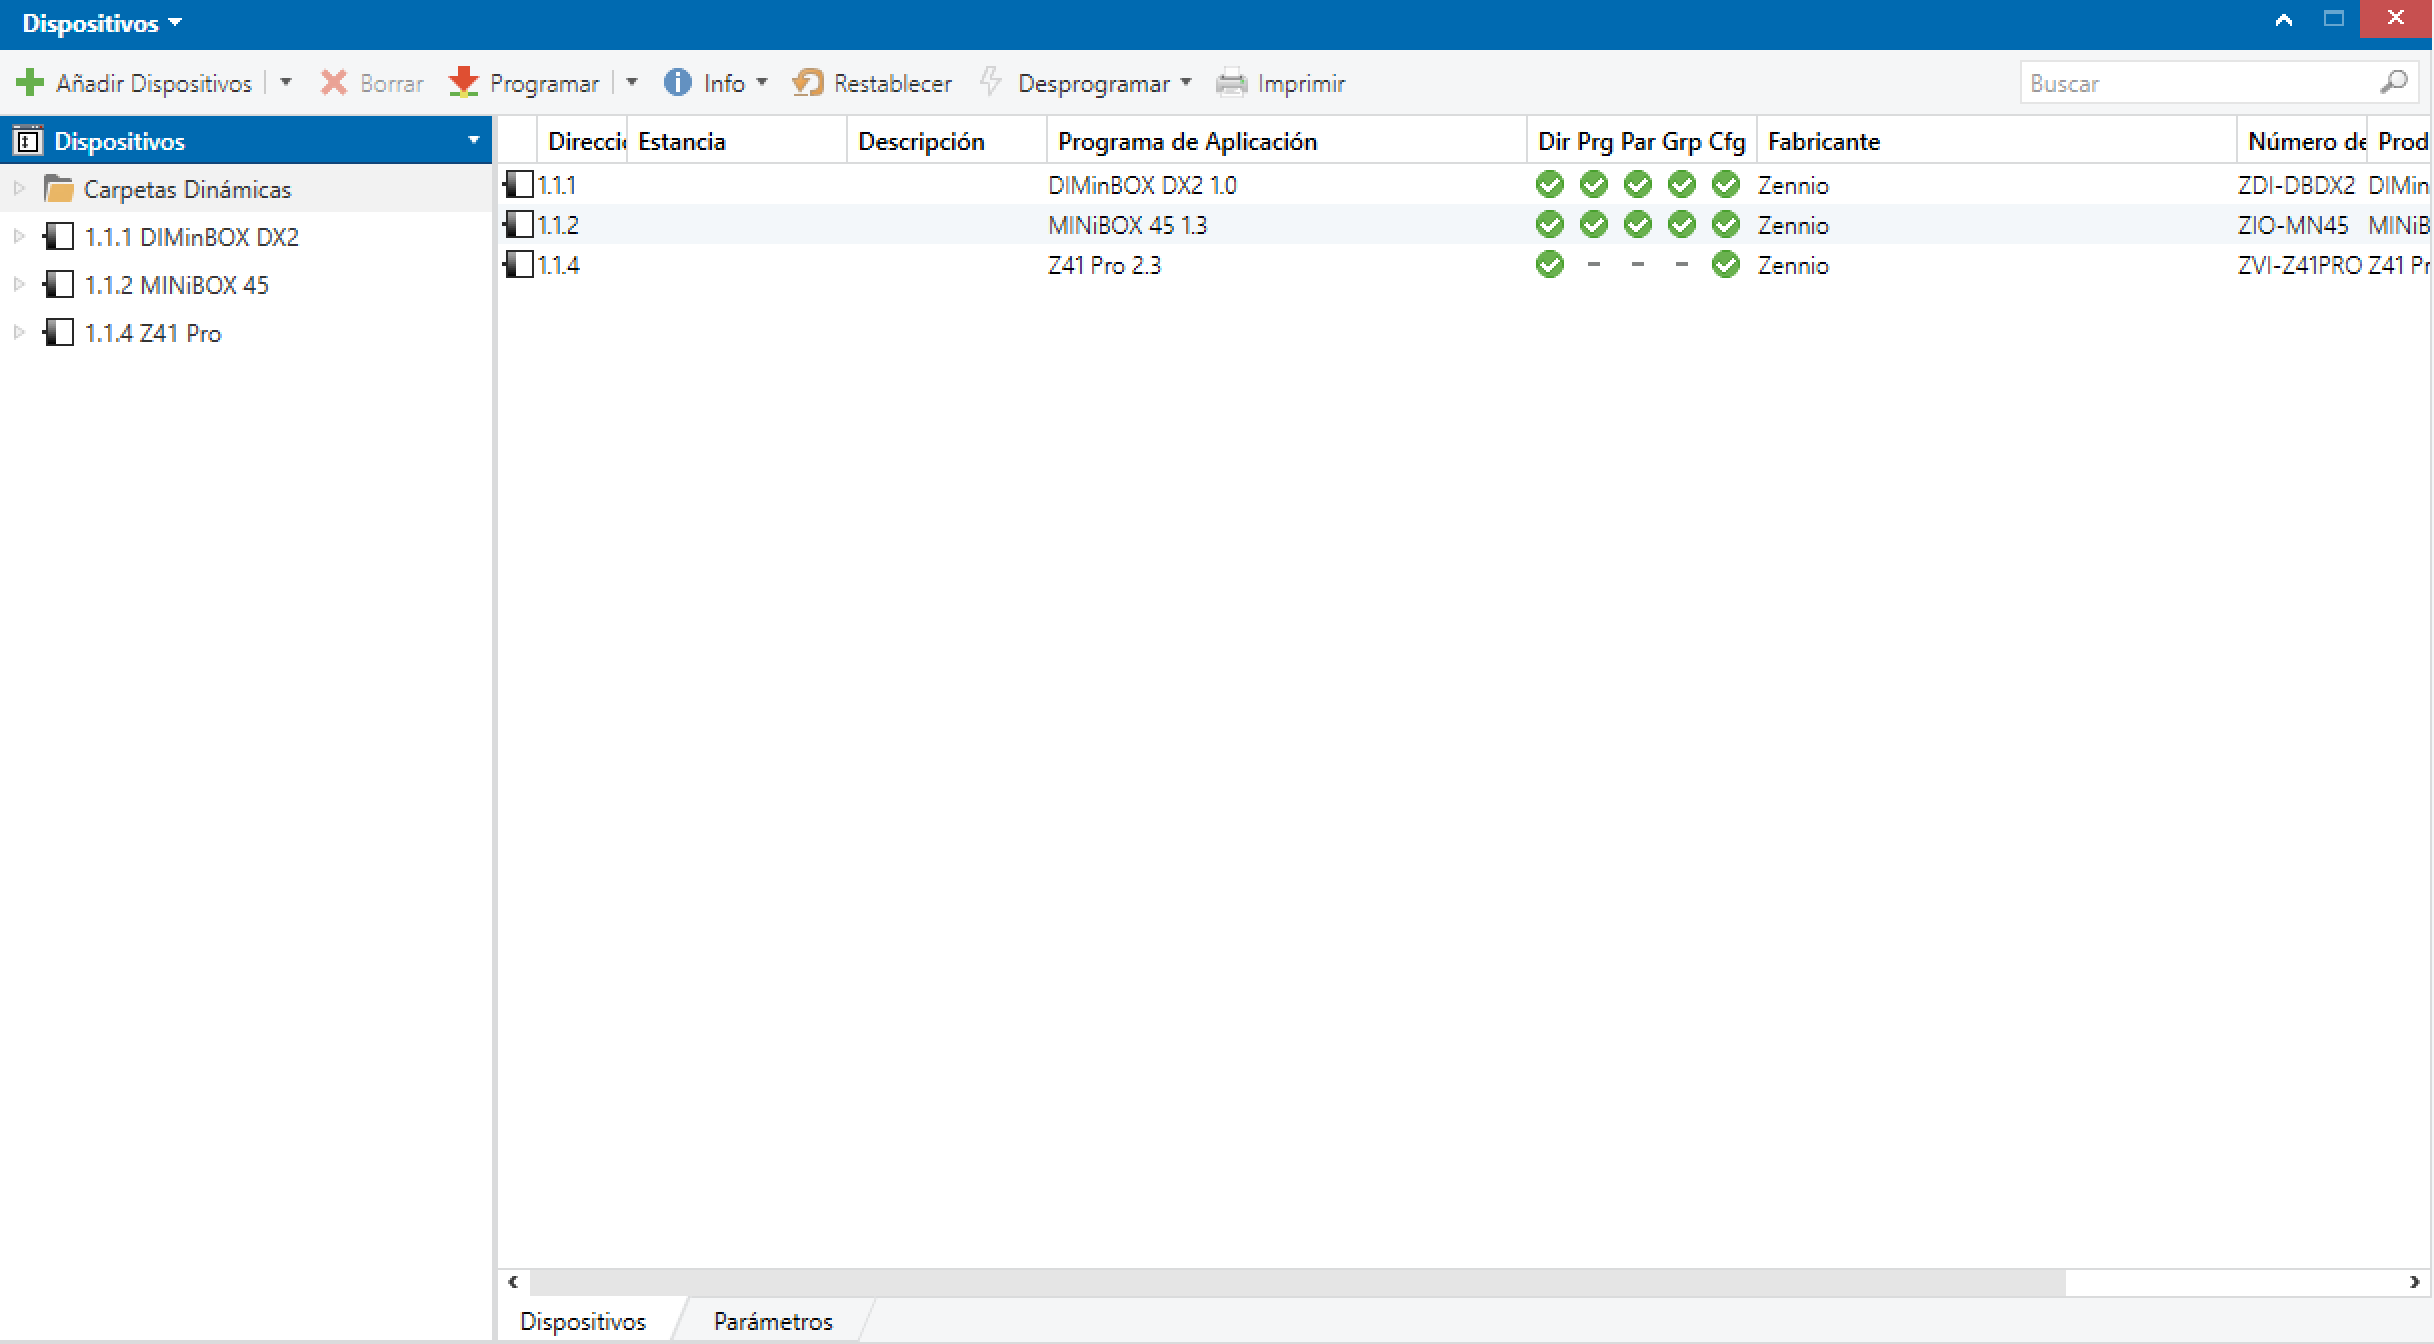
\includegraphics[width = 1.00\textwidth]{Imagenes/img19}
 		\captionof{figure}{\label{fig:IPN}Agregando dispositivos.} 
	\end{center} 
\end{figure}

El primer dispositivo que vamos a configurar es el \textbf{DIMinBOX DX2}, más concretamente la entrada 1 (\textbf{E1}) correspondiente a la sonda de temperatura a la cual le estableceremos un periodo de 10 segundos de envío de temperatura, así como el envío tras un cambio de 0.1ºC de temperatura como se muestra en la siguiente figura. \\

\begin{figure}[H]
	\begin{center}
	 		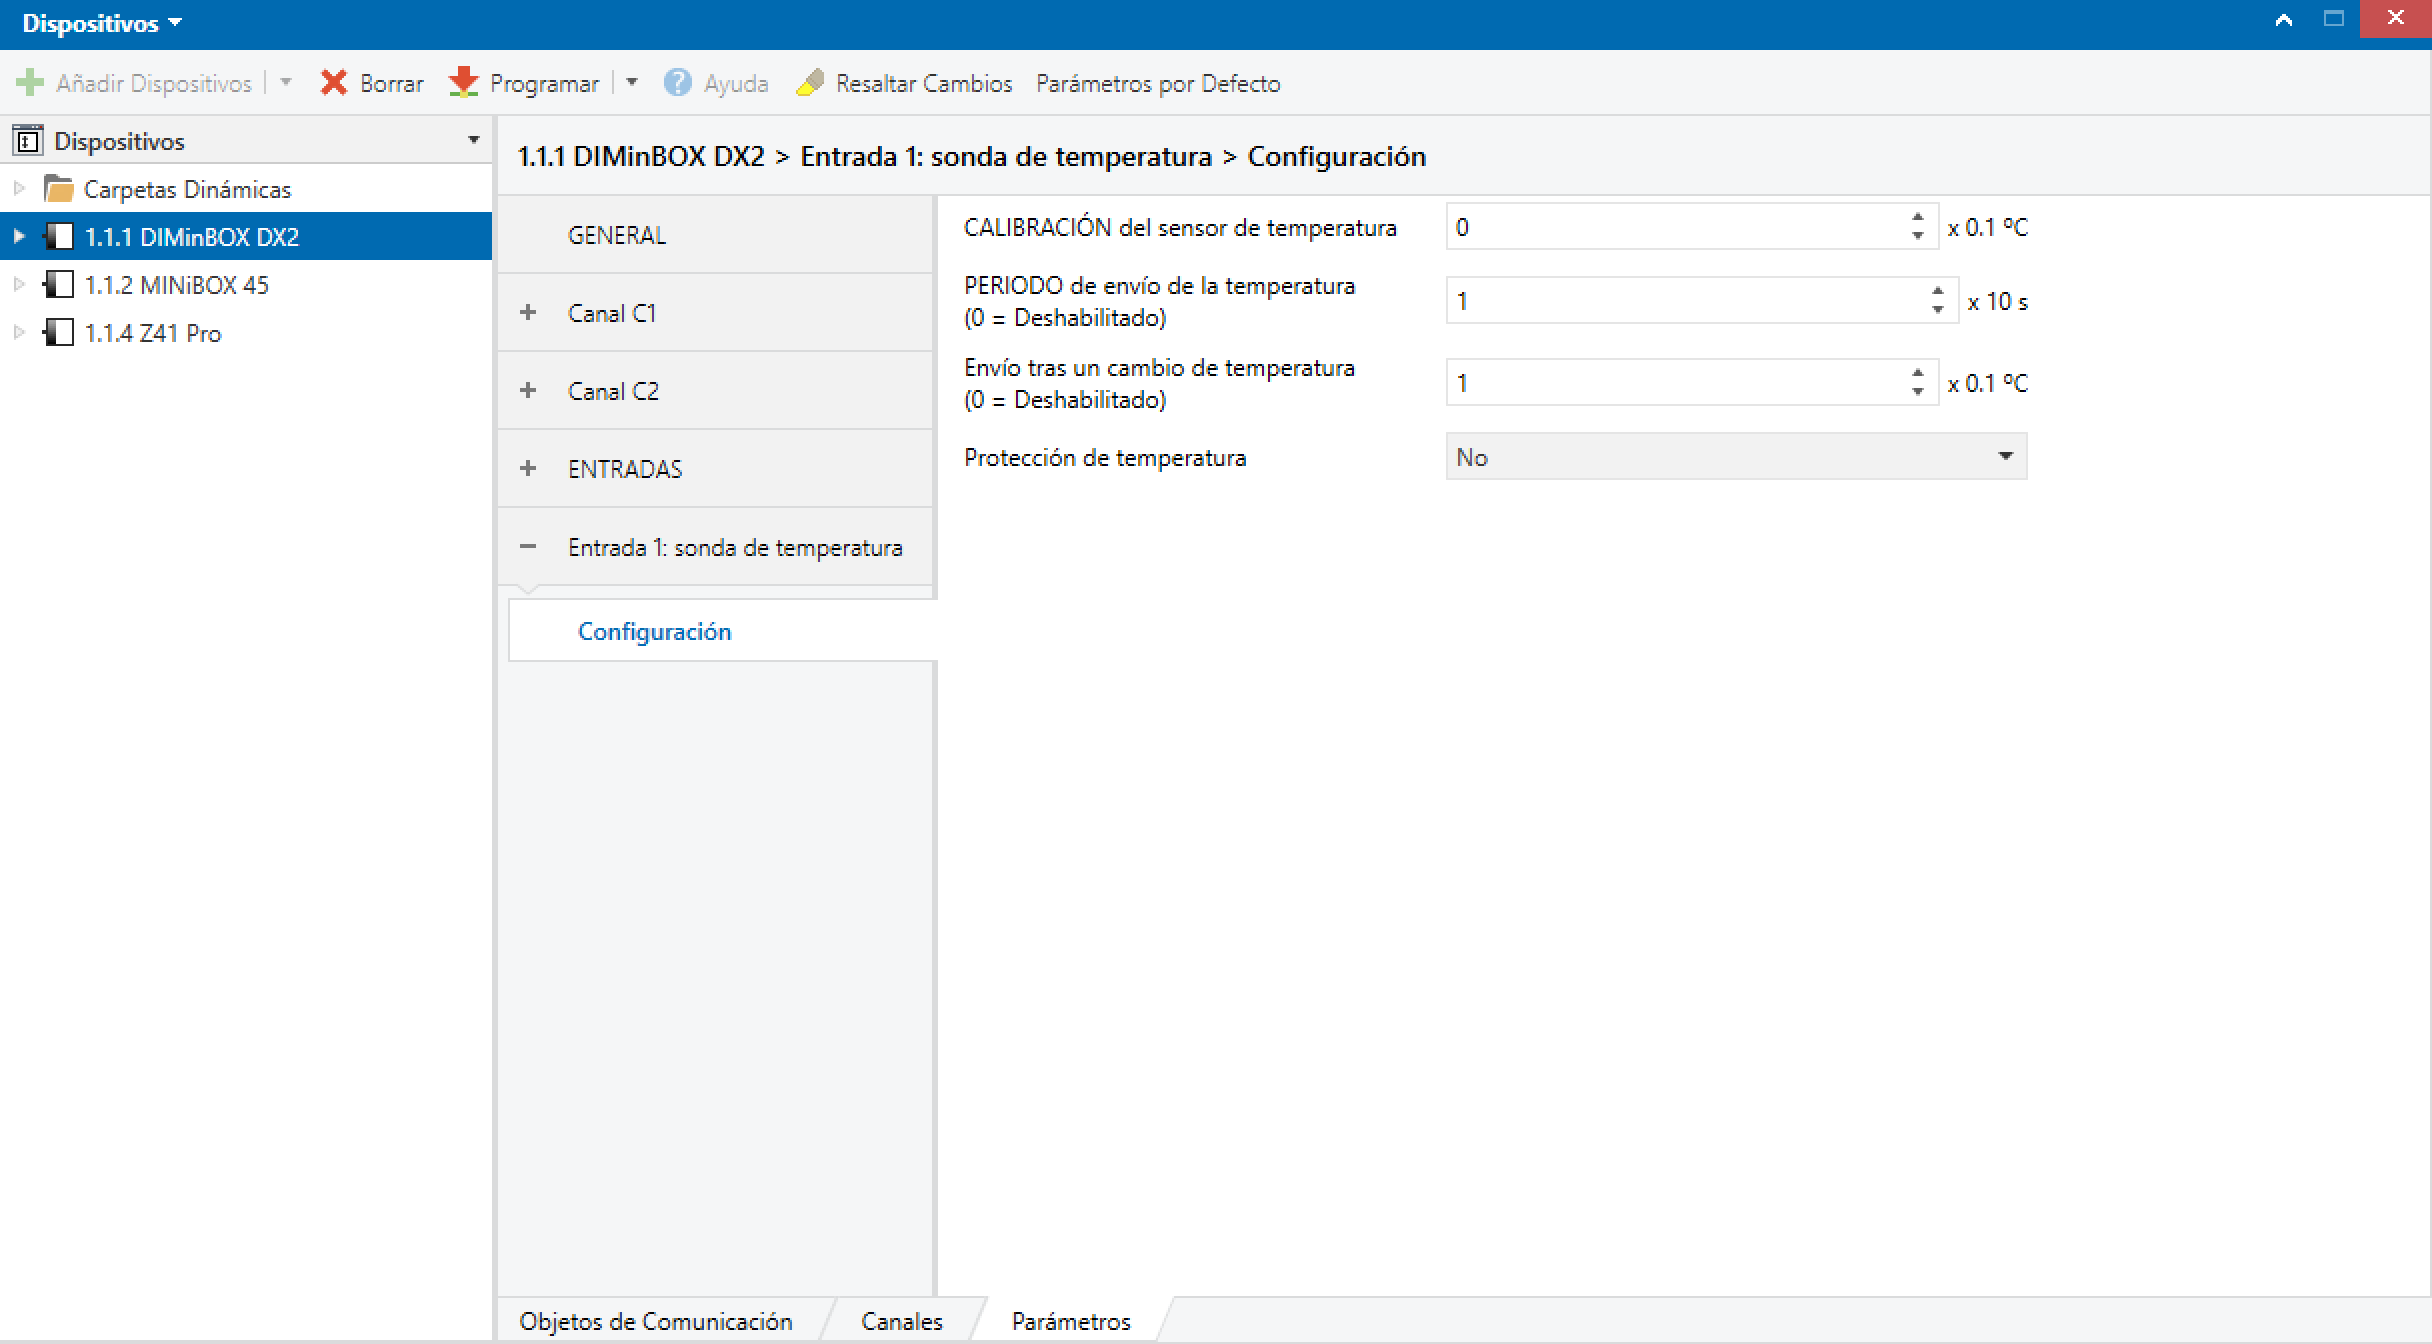
\includegraphics[width = 1.00\textwidth]{Imagenes/img20}
 		\captionof{figure}{\label{fig:IPN}Configurando la entrada 1 del \textbf{DIMinBOX DX2}.} 
	\end{center} 
\end{figure}

El siguiente dispositivo a configurar es el \textbf{MINiBOX 45} el cual dispone de cuatro salidas de las que vamos a utilizar la salida 3 y cuyo control especificaremos que será manual. En la parametrización de la salida 3 estableceremos el tipo a normalmente abierto asi como el arranque por defecto.  La configuración del control manual la dejaremos por defecto. \\


\begin{figure}[H]
	\begin{center}
	 		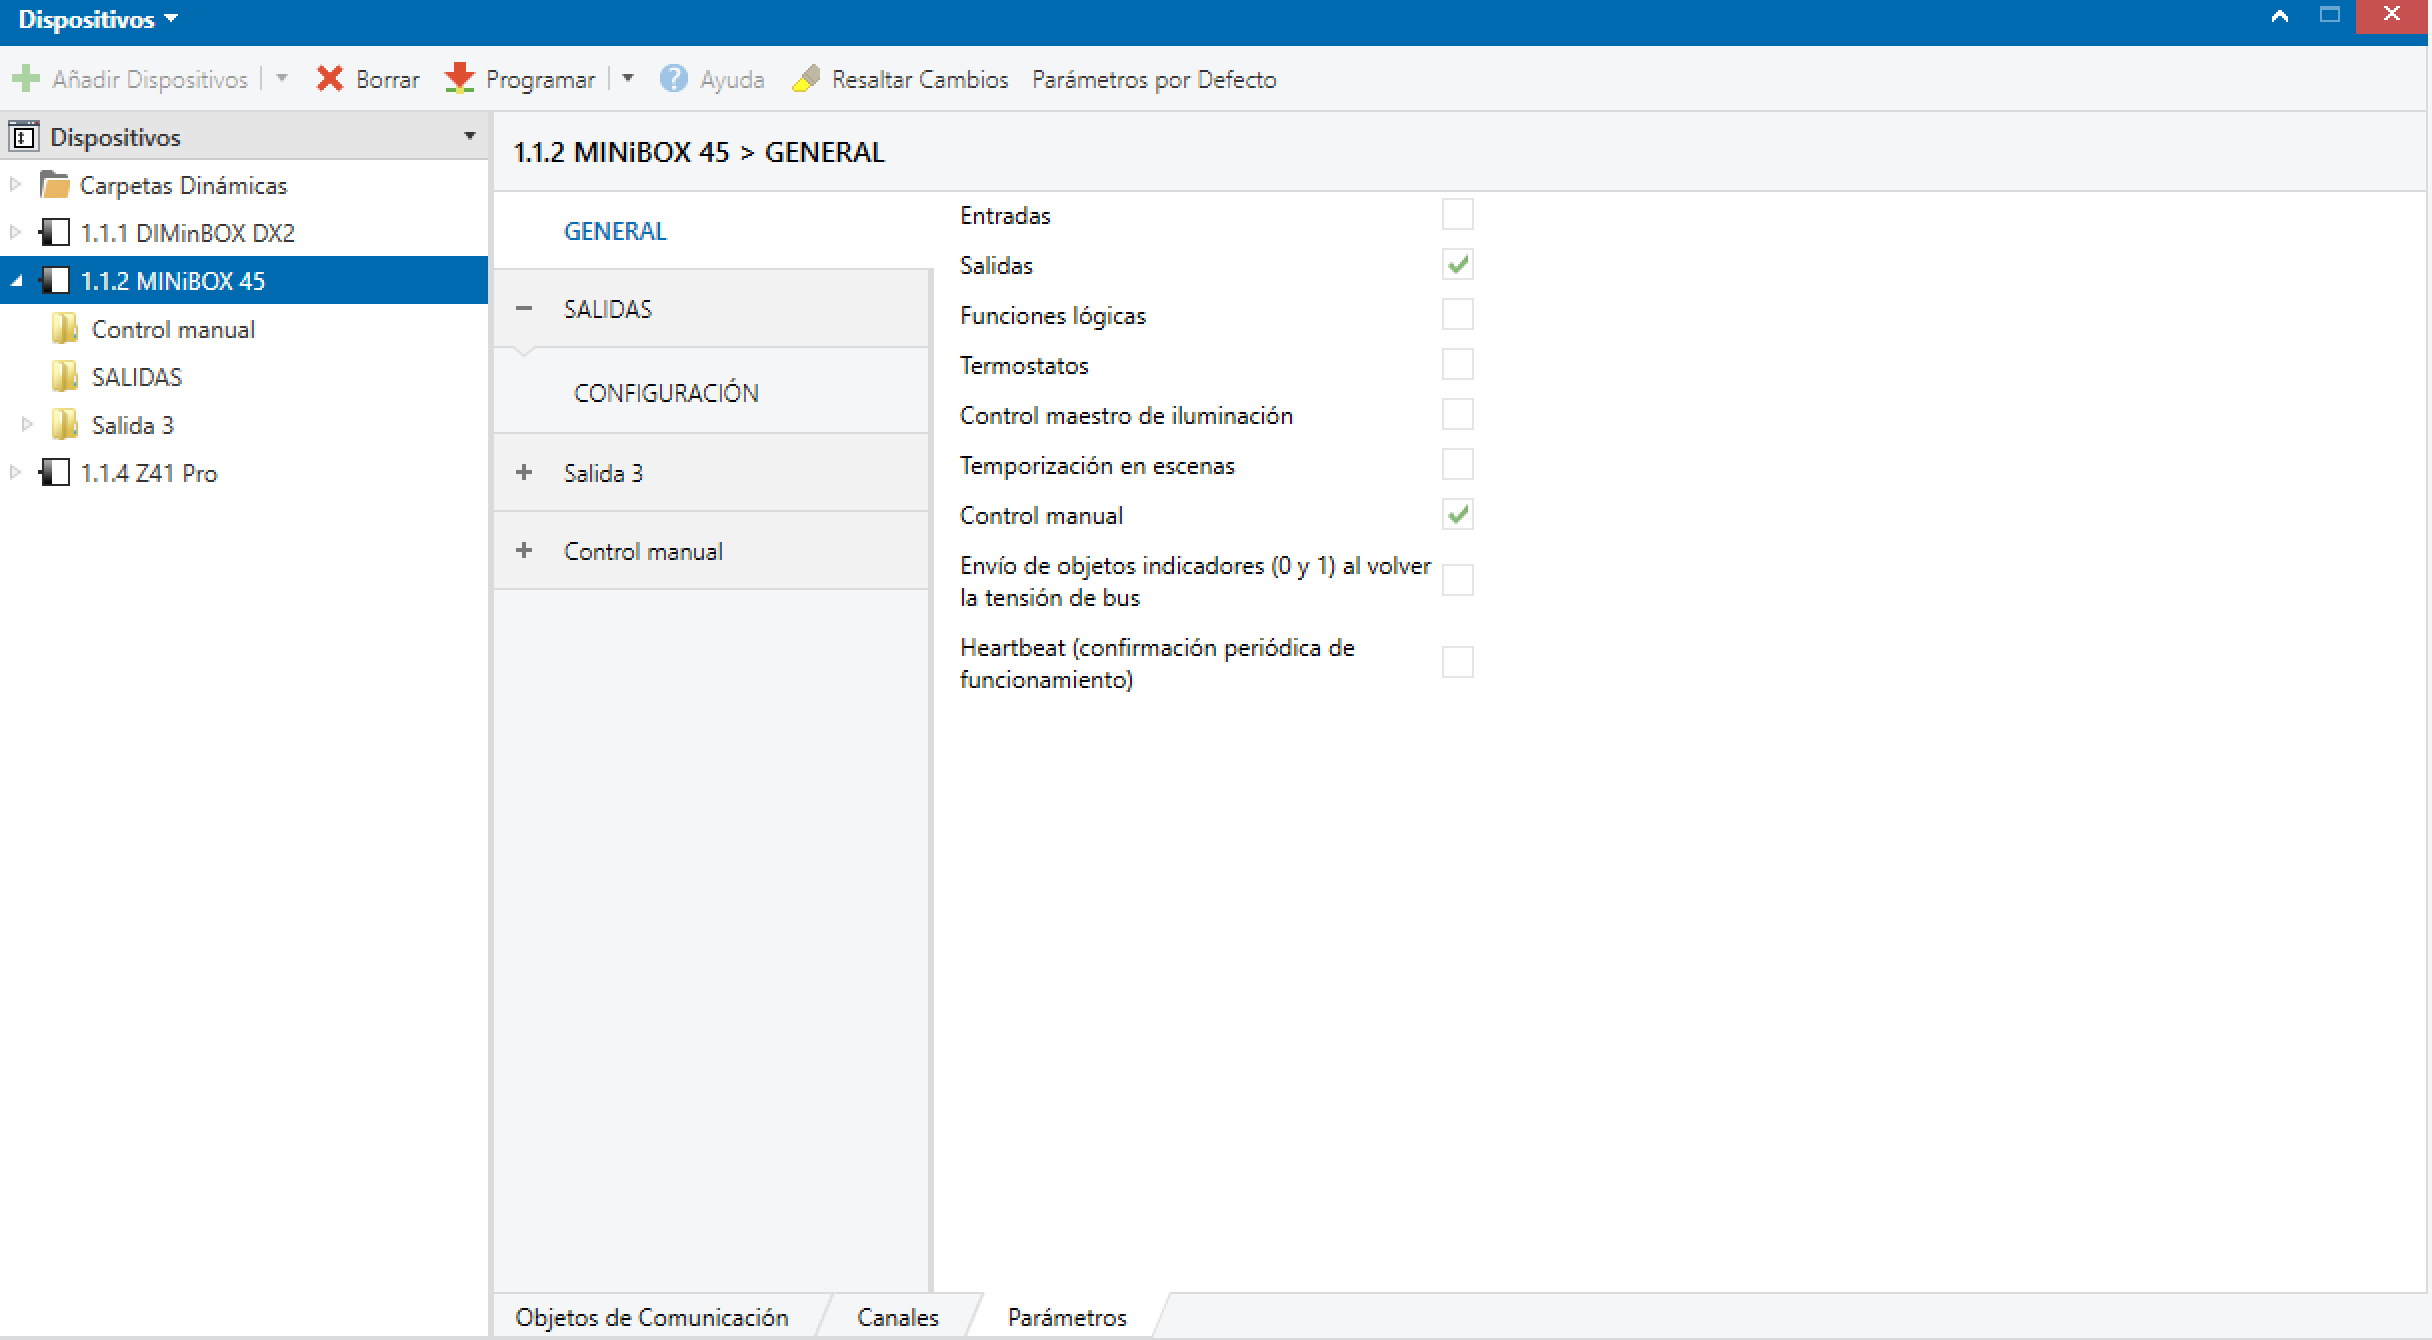
\includegraphics[width = 1.00\textwidth]{Imagenes/img21}
 		\captionof{figure}{\label{fig:IPN}Configurando dispositivo \textbf{MINiBOX 45}.} 
	\end{center} 
\end{figure}

\begin{figure}[H]
	\begin{center}
	 		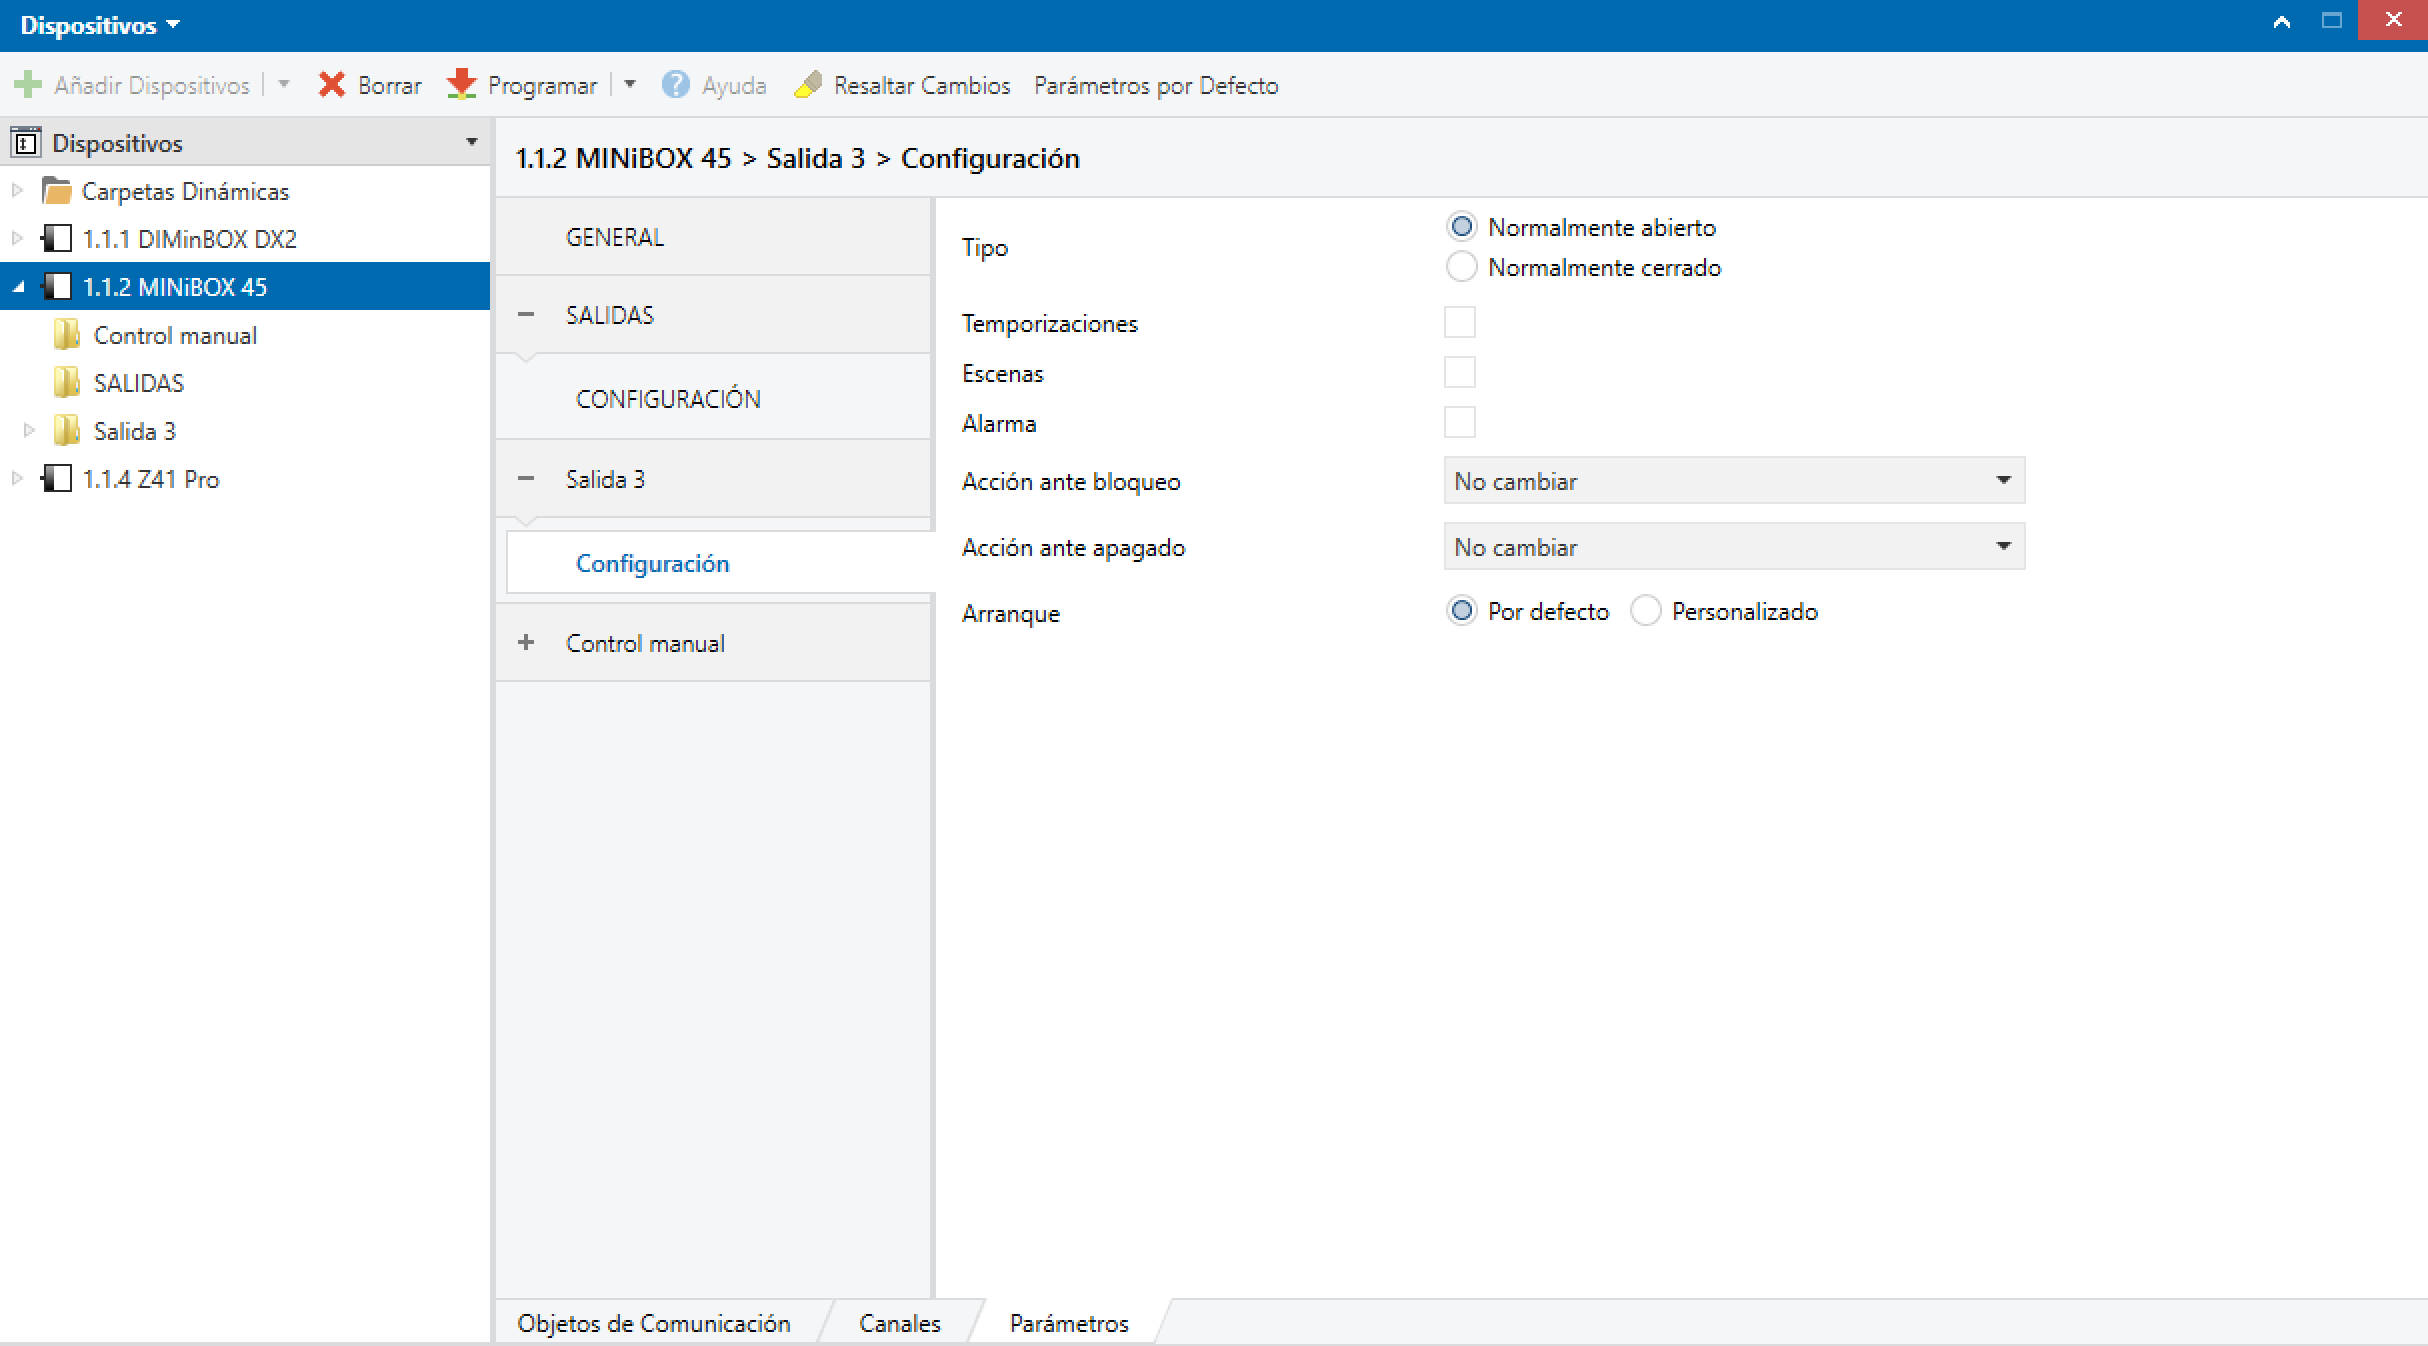
\includegraphics[width = 1.00\textwidth]{Imagenes/img22}
 		\captionof{figure}{\label{fig:IPN}Configurando salida 3 del \textbf{MINiBOX 45}.} 
	\end{center} 
\end{figure}

\begin{figure}[H]
	\begin{center}
	 		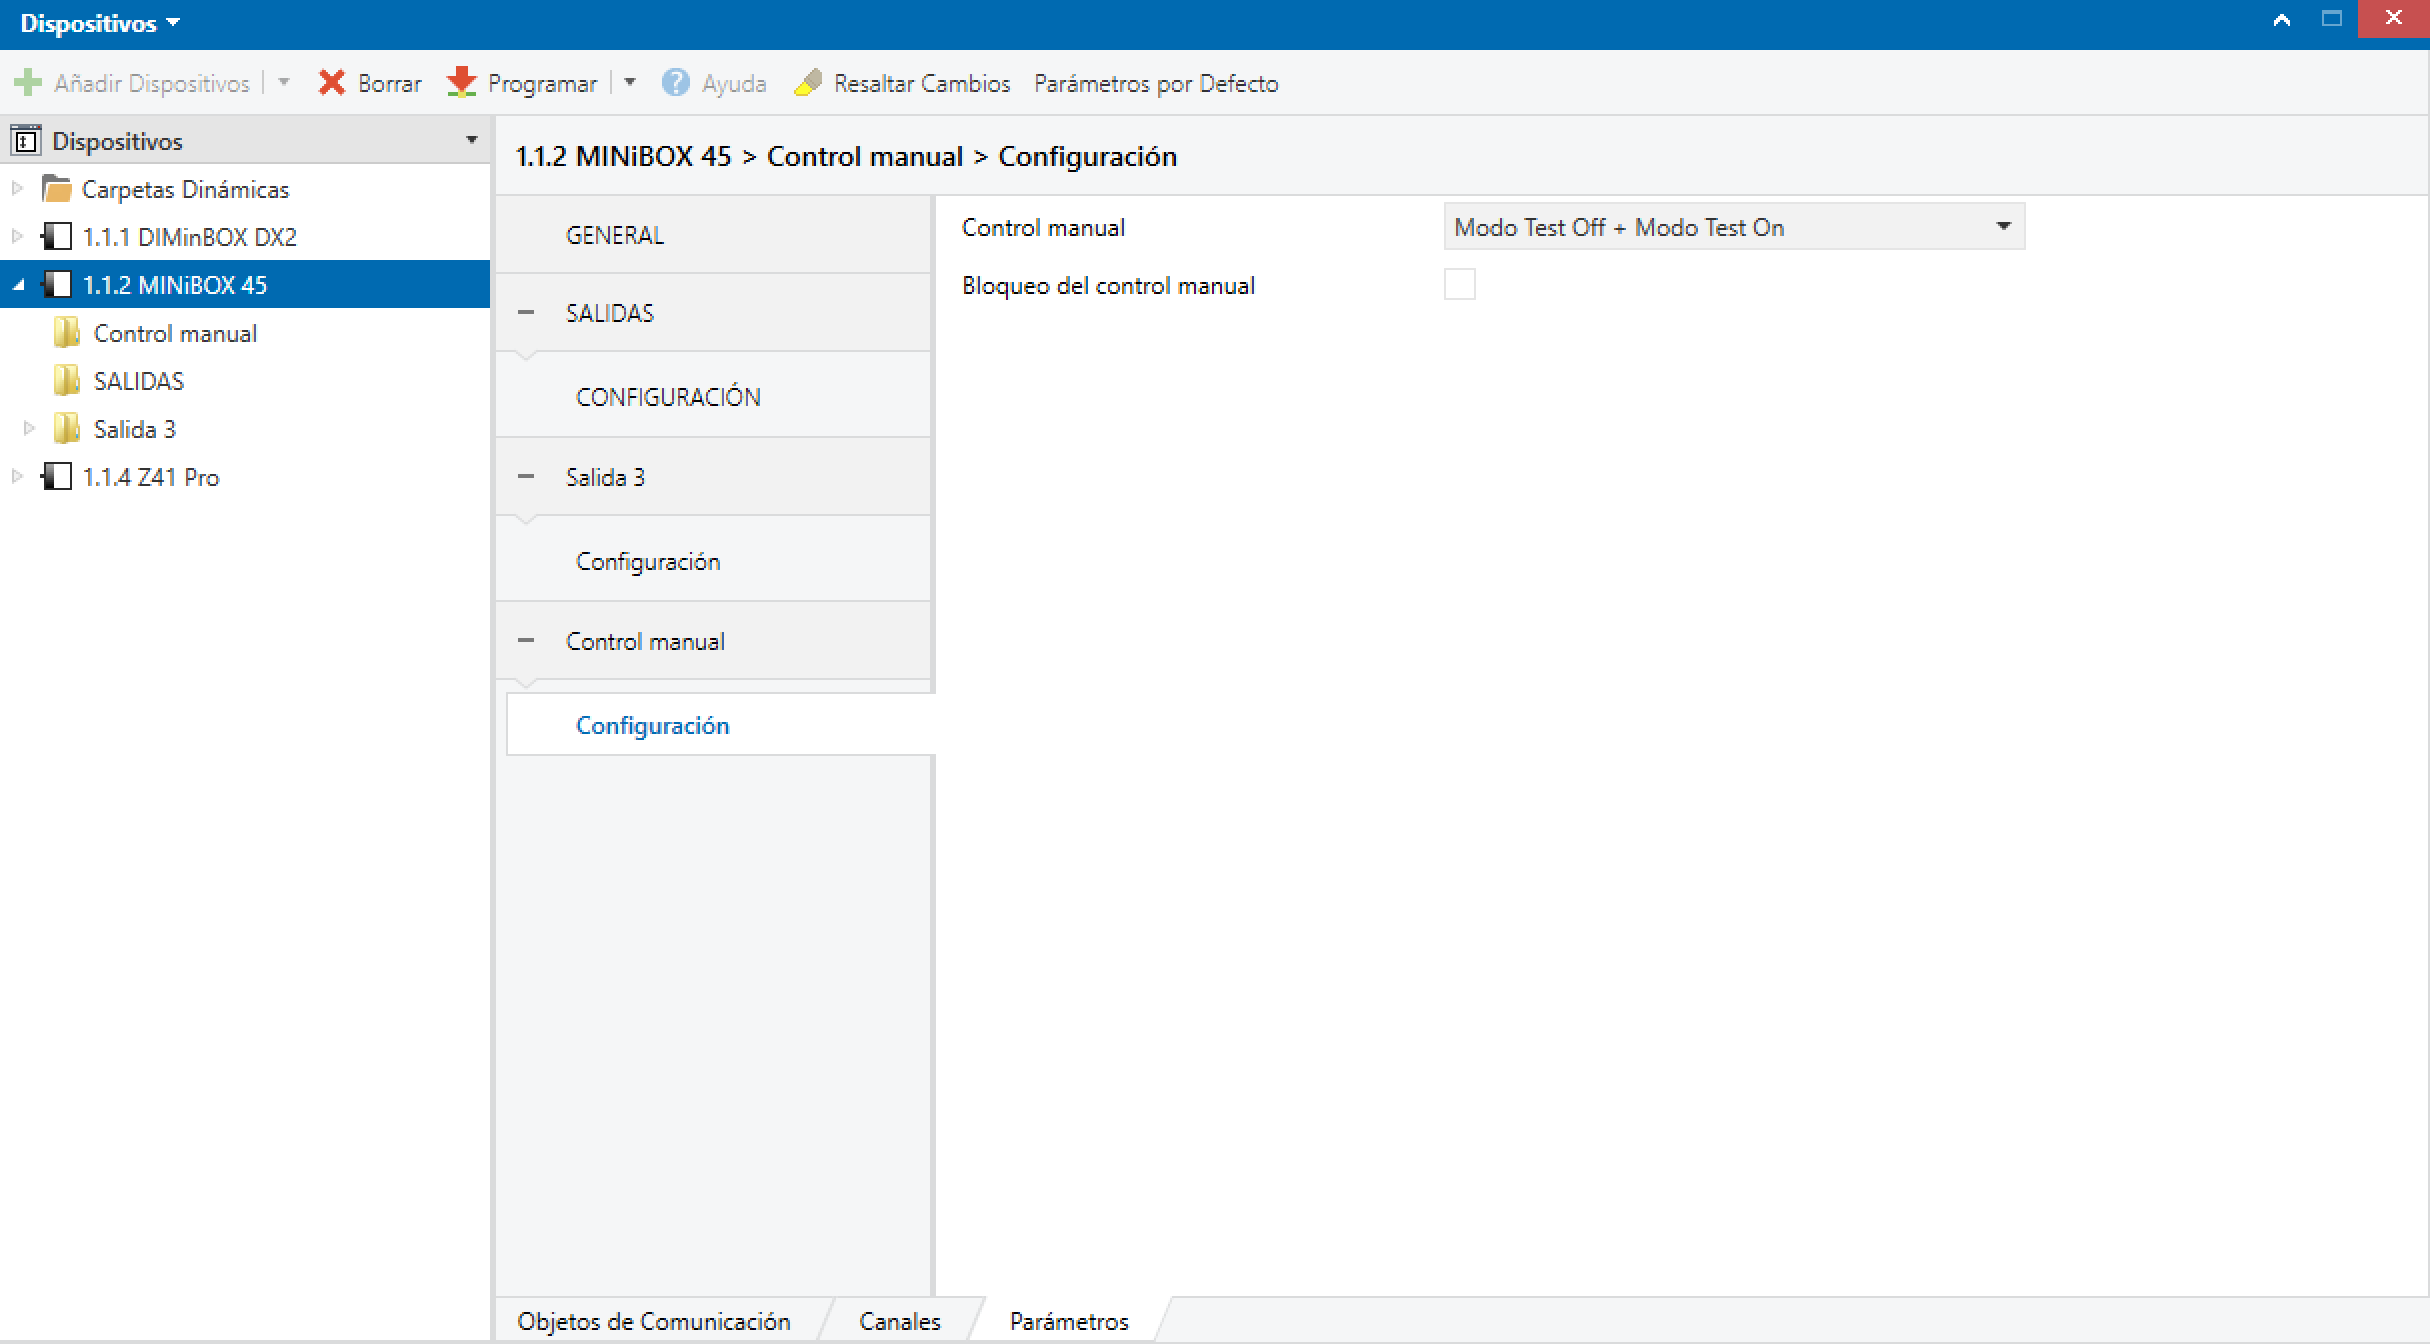
\includegraphics[width = 1.00\textwidth]{Imagenes/img23}
 		\captionof{figure}{\label{fig:IPN}Configurando control manual del \textbf{MINiBOX 45}.} 
	\end{center} 
\end{figure}

El último dispositivo a configurar es el \textbf{Z41 Pro} el cual dispone de dos termostatos. Parametrizaremos uno de ellos (\textbf{Termostato 1}) para regular la temperatura cuando esta sea diferente a la de consigna. El panel táctil estará conectado a una fuente de alimentación de 29V y se utilizará en orientación vertical. \\

\begin{figure}[H]
	\begin{center}
	 		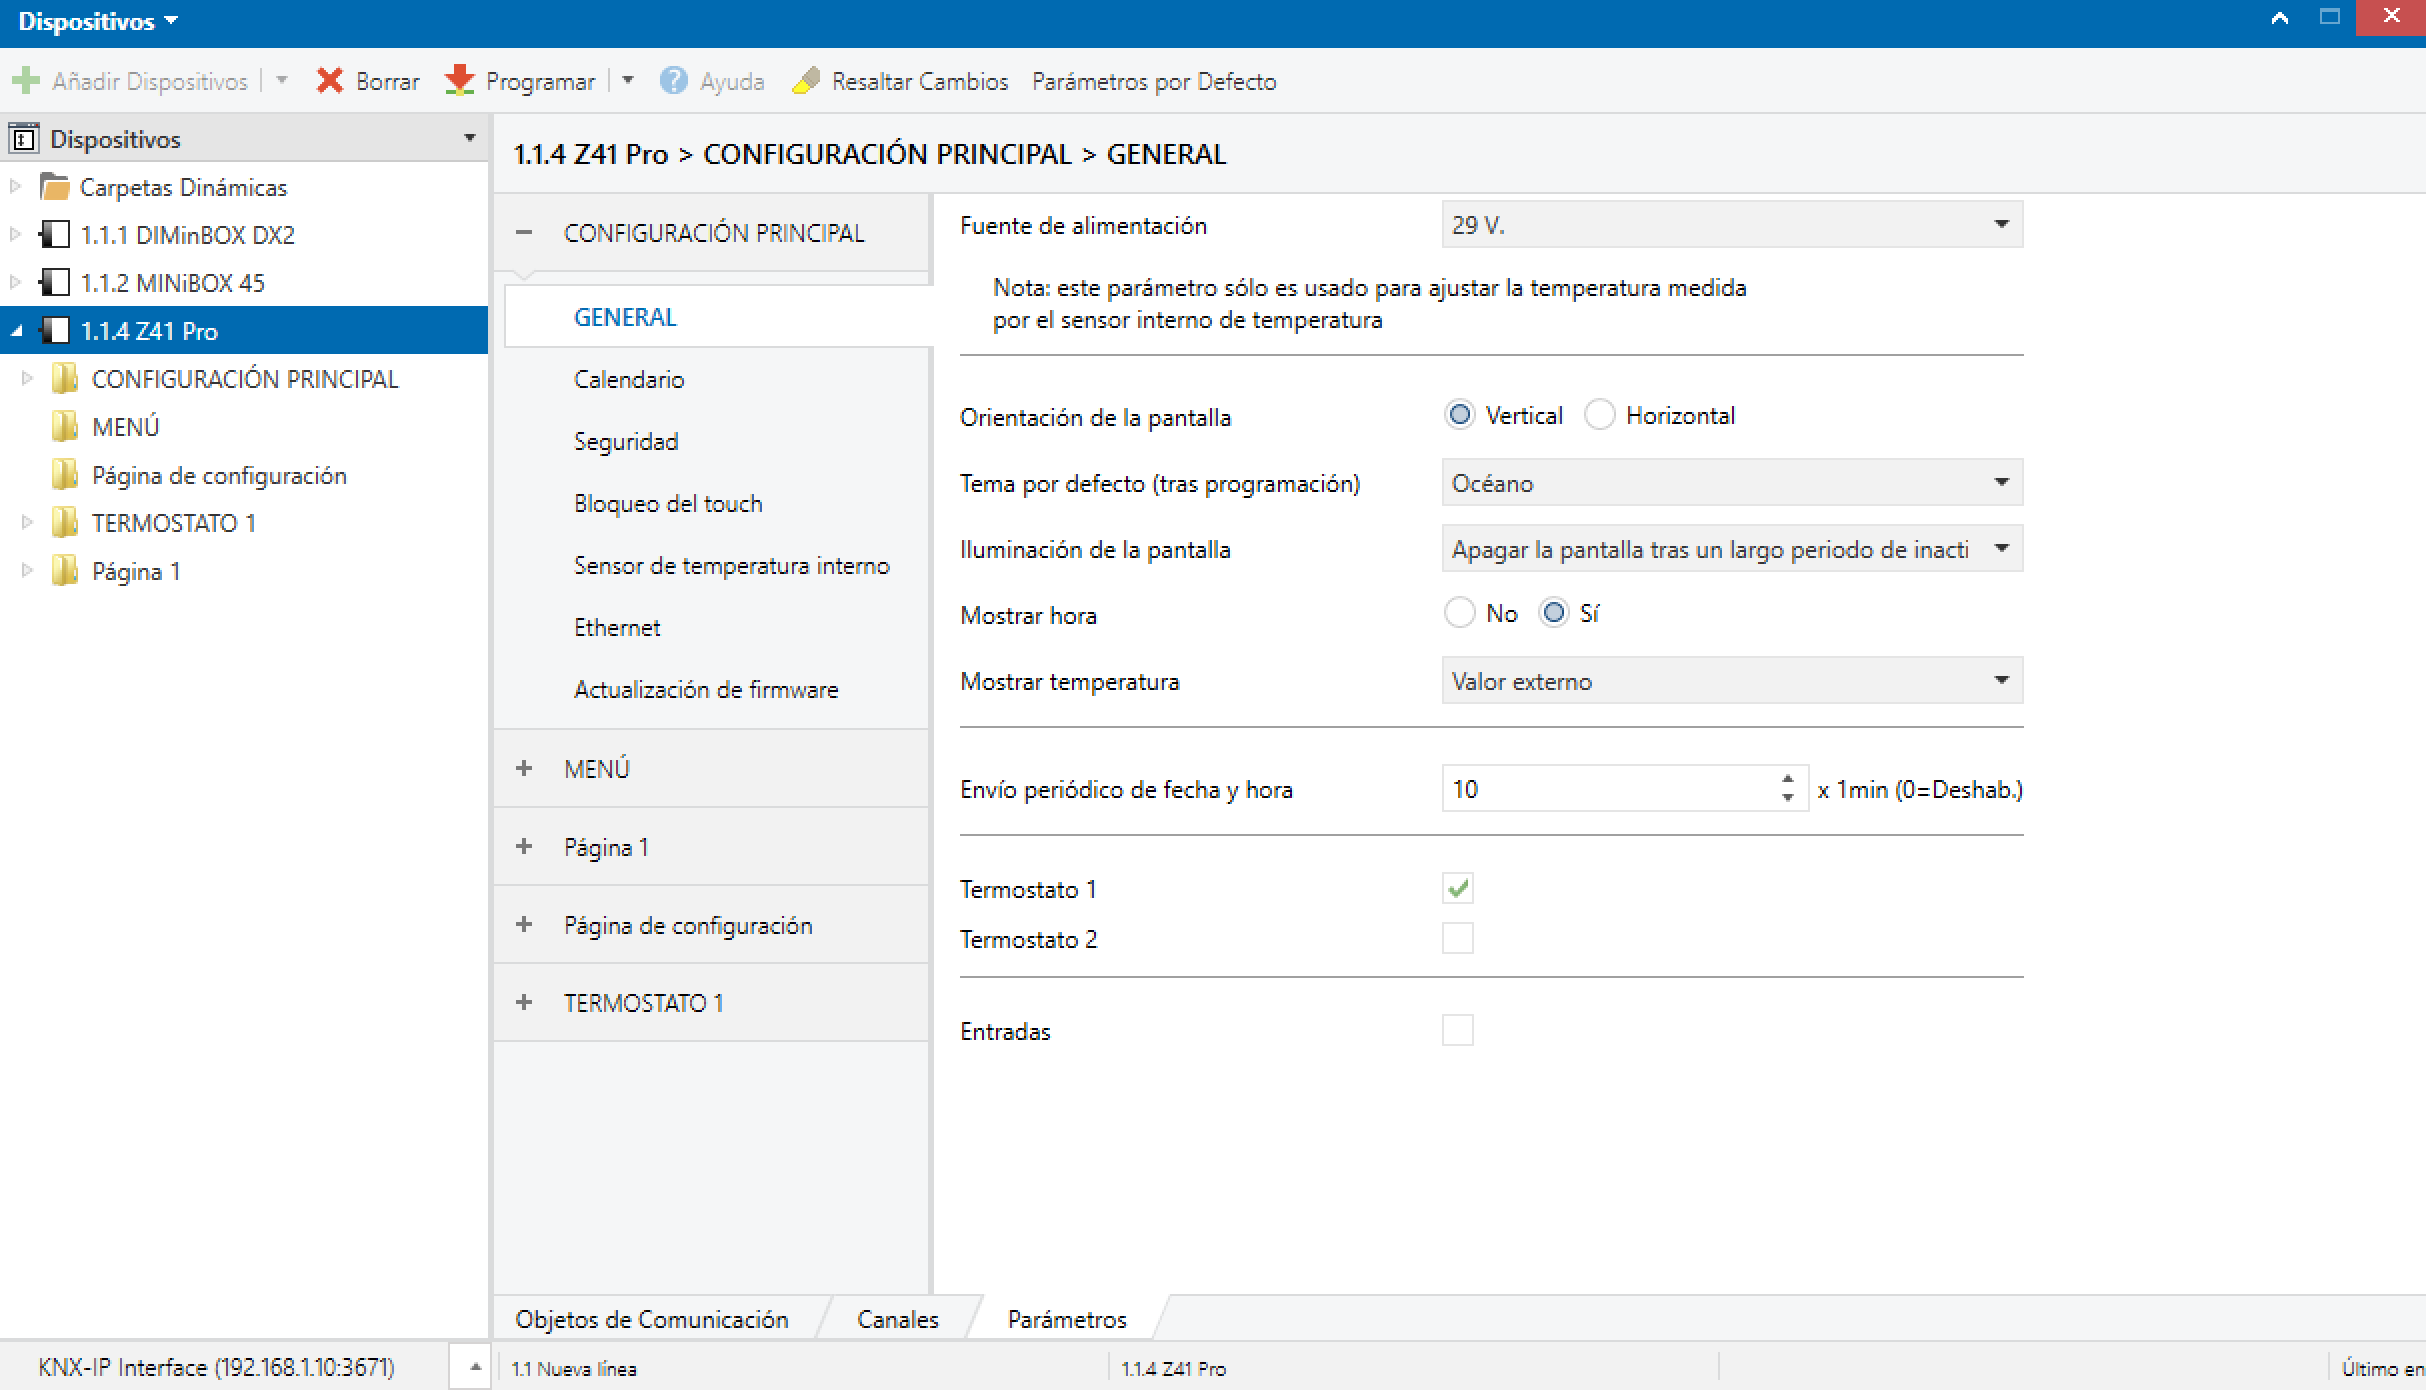
\includegraphics[width = 1.00\textwidth]{Imagenes/img24}
 		\captionof{figure}{\label{fig:IPN}Configurando dispositivo \textbf{Z41 Pro} (I).} 
	\end{center} 
\end{figure}

Utilizaremos la página 1 de dicho panel y la casilla 1 dentro de la misma. Su función será la de mostrar la temperatura la cual tendrá un valor mínimo de 15º y un valor máximo de 30º. Se utilizará el botón izquierdo de dicho panel para bajar temperatura y el botón derecho para subirla. \\

\begin{figure}[H]
	\begin{center}
	 		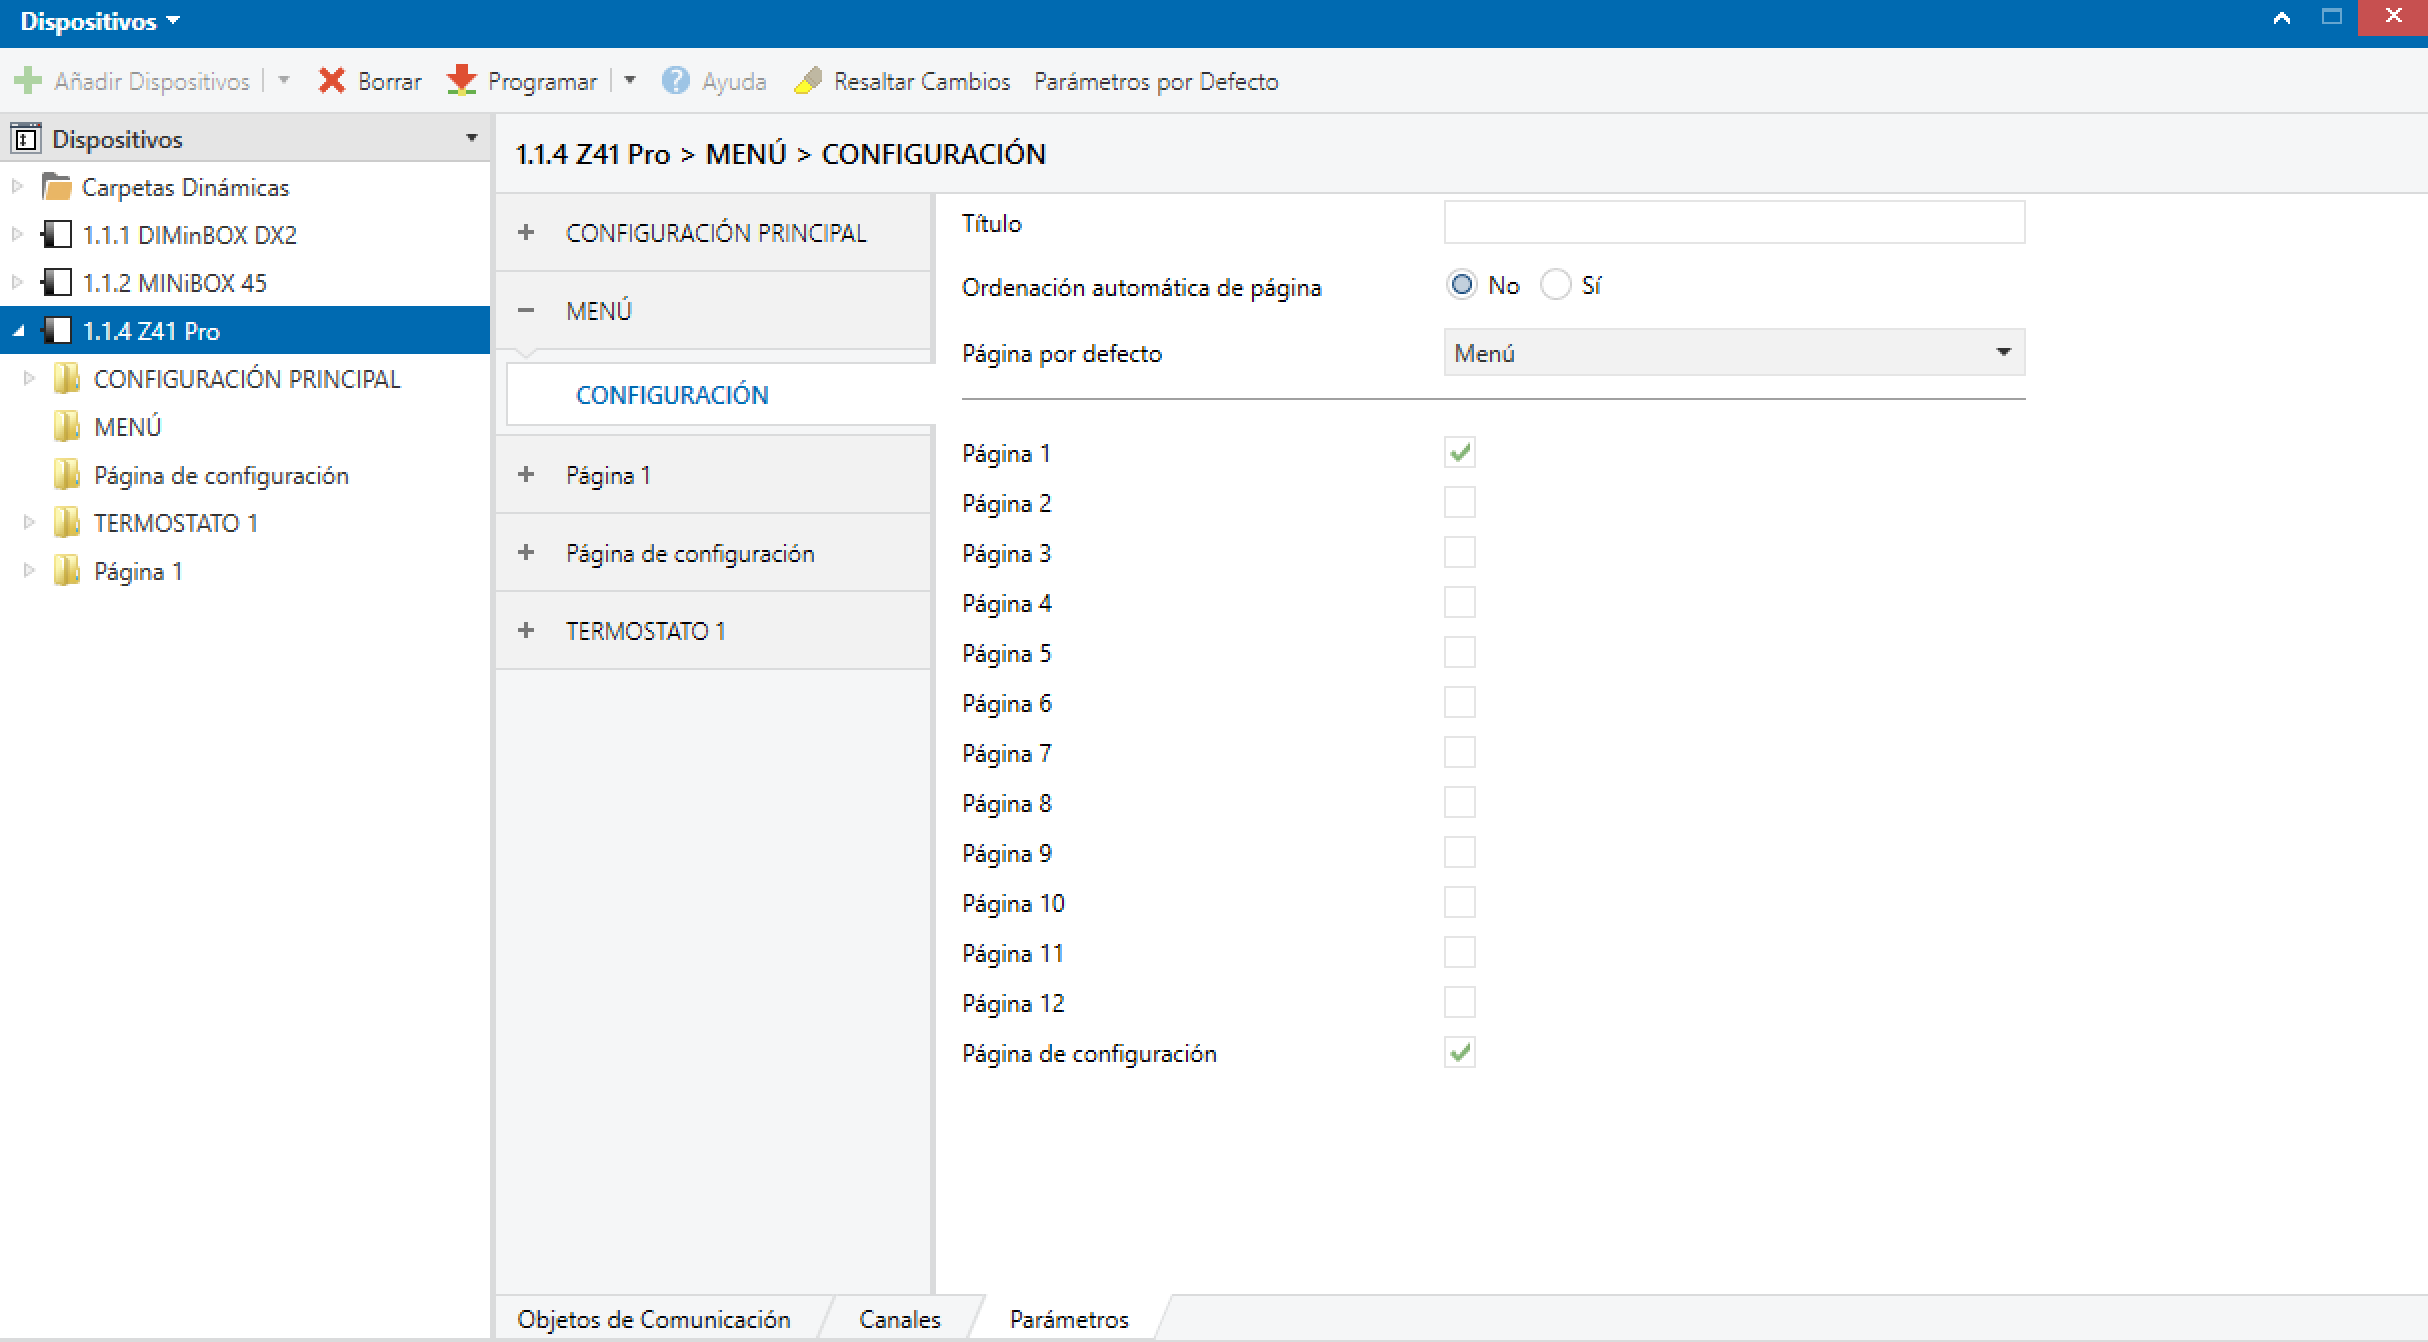
\includegraphics[width = 1.00\textwidth]{Imagenes/img25}
 		\captionof{figure}{\label{fig:IPN}Configurando dispositivo \textbf{Z41 Pro} (II).} 
	\end{center} 
\end{figure}

\begin{figure}[H]
	\begin{center}
	 		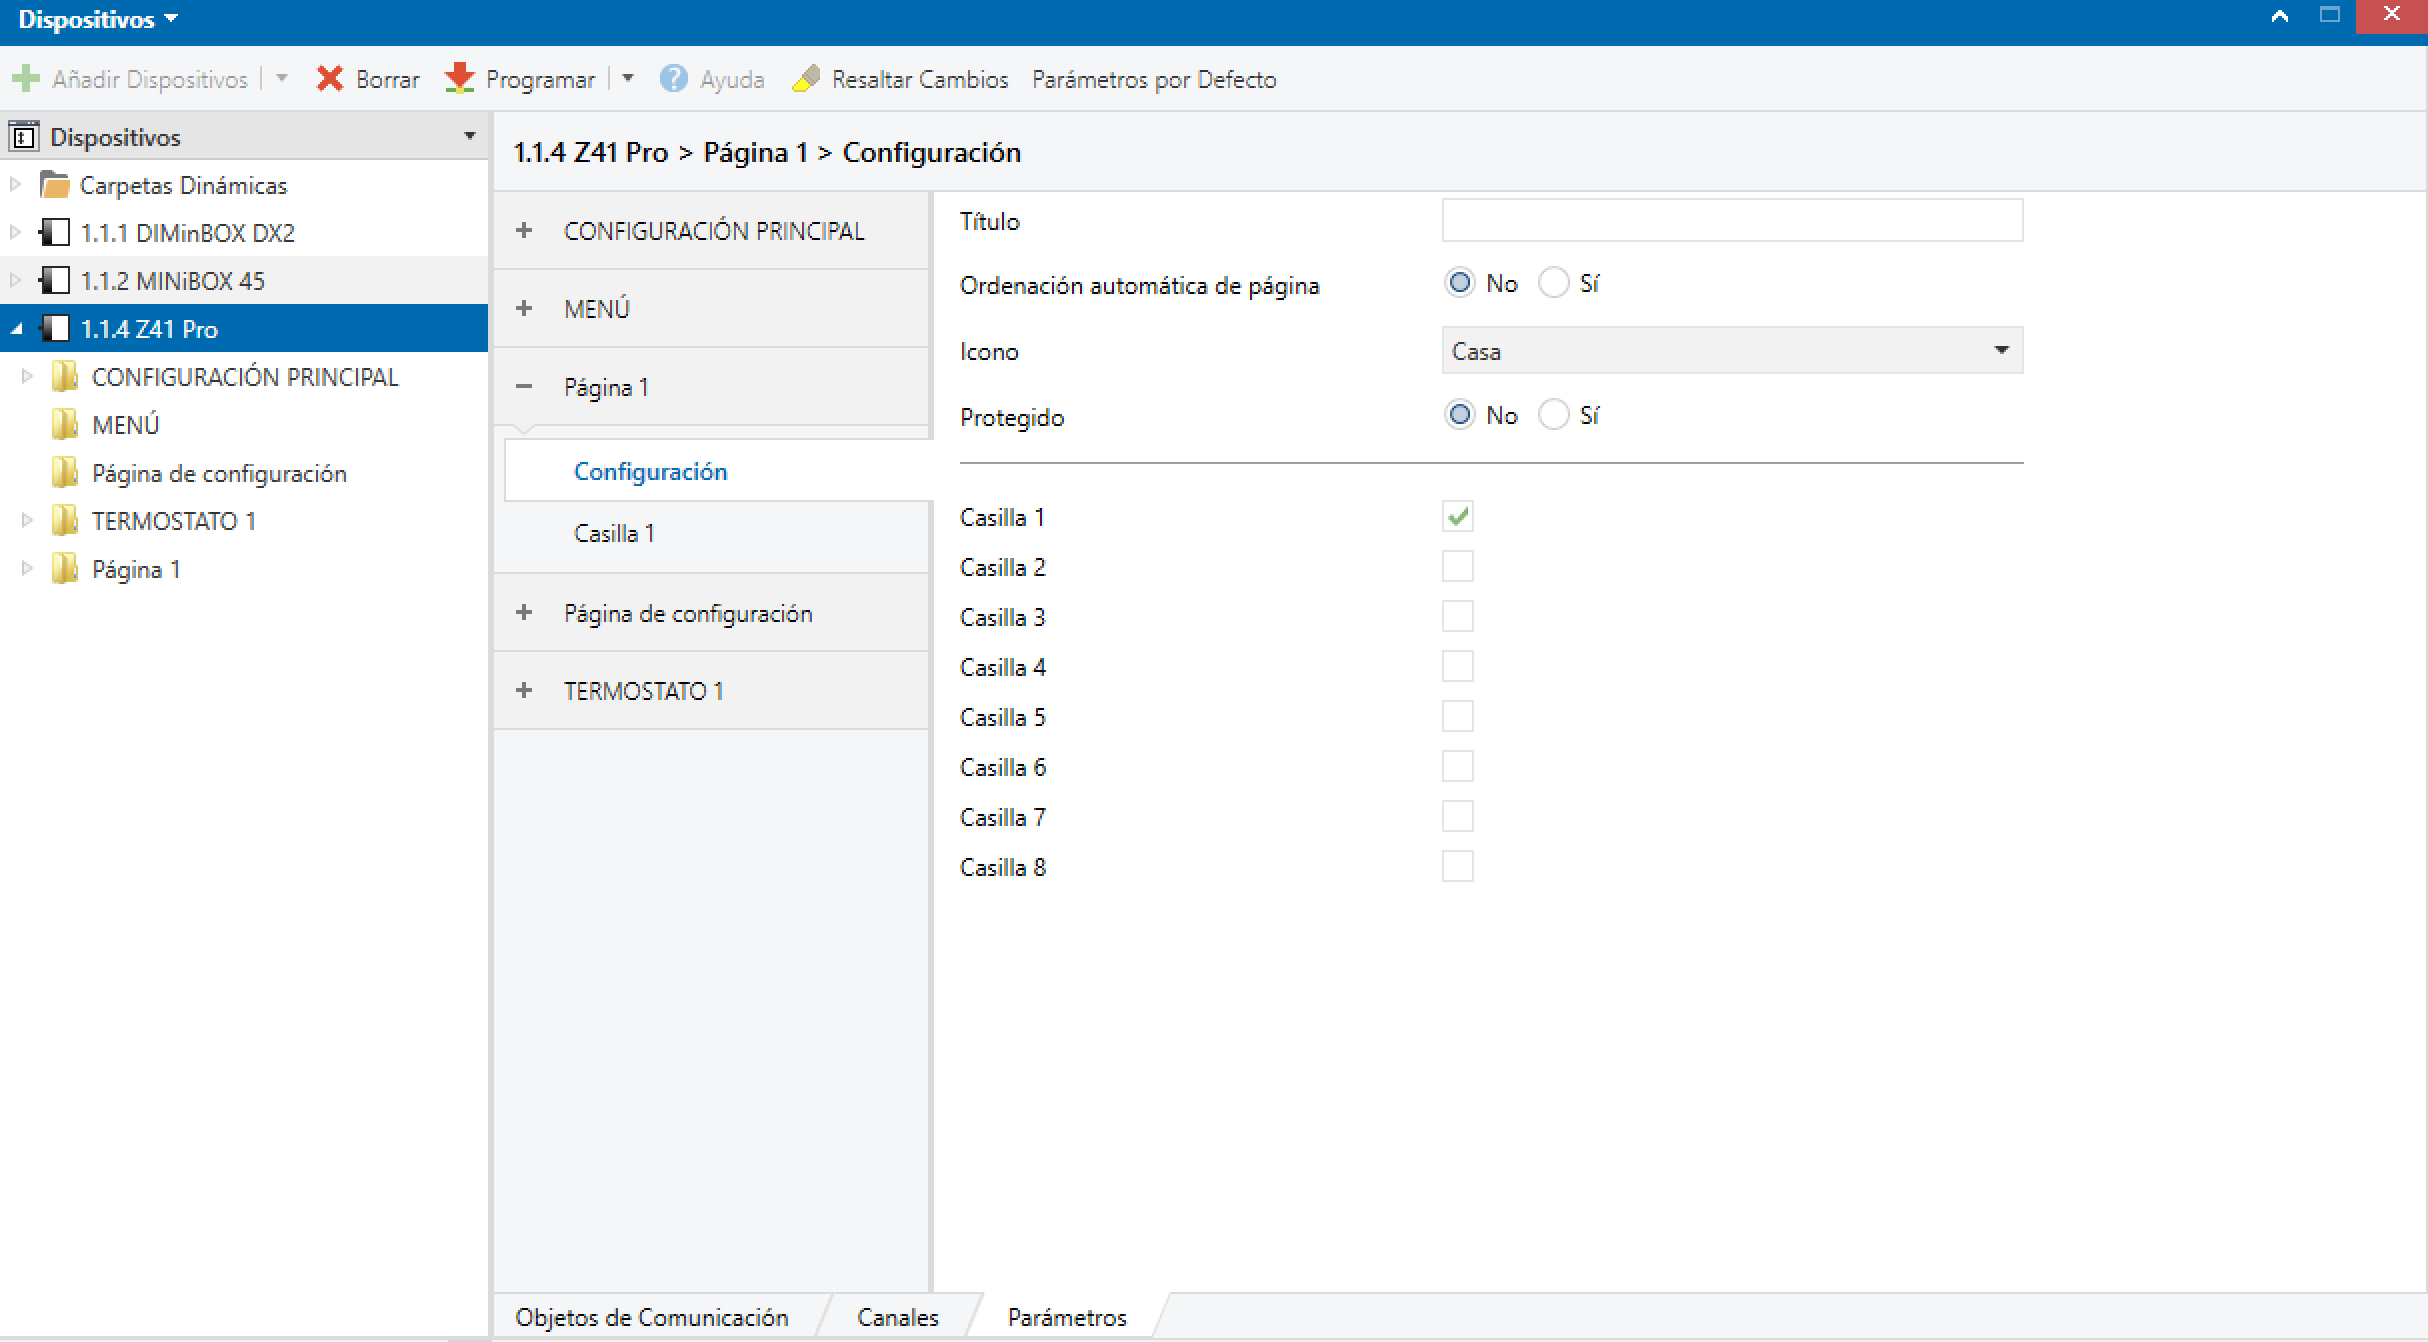
\includegraphics[width = 1.00\textwidth]{Imagenes/img26}
 		\captionof{figure}{\label{fig:IPN}Configurando dispositivo \textbf{Z41 Pro} (III).} 
	\end{center} 
\end{figure}

\begin{figure}[H]
	\begin{center}
	 		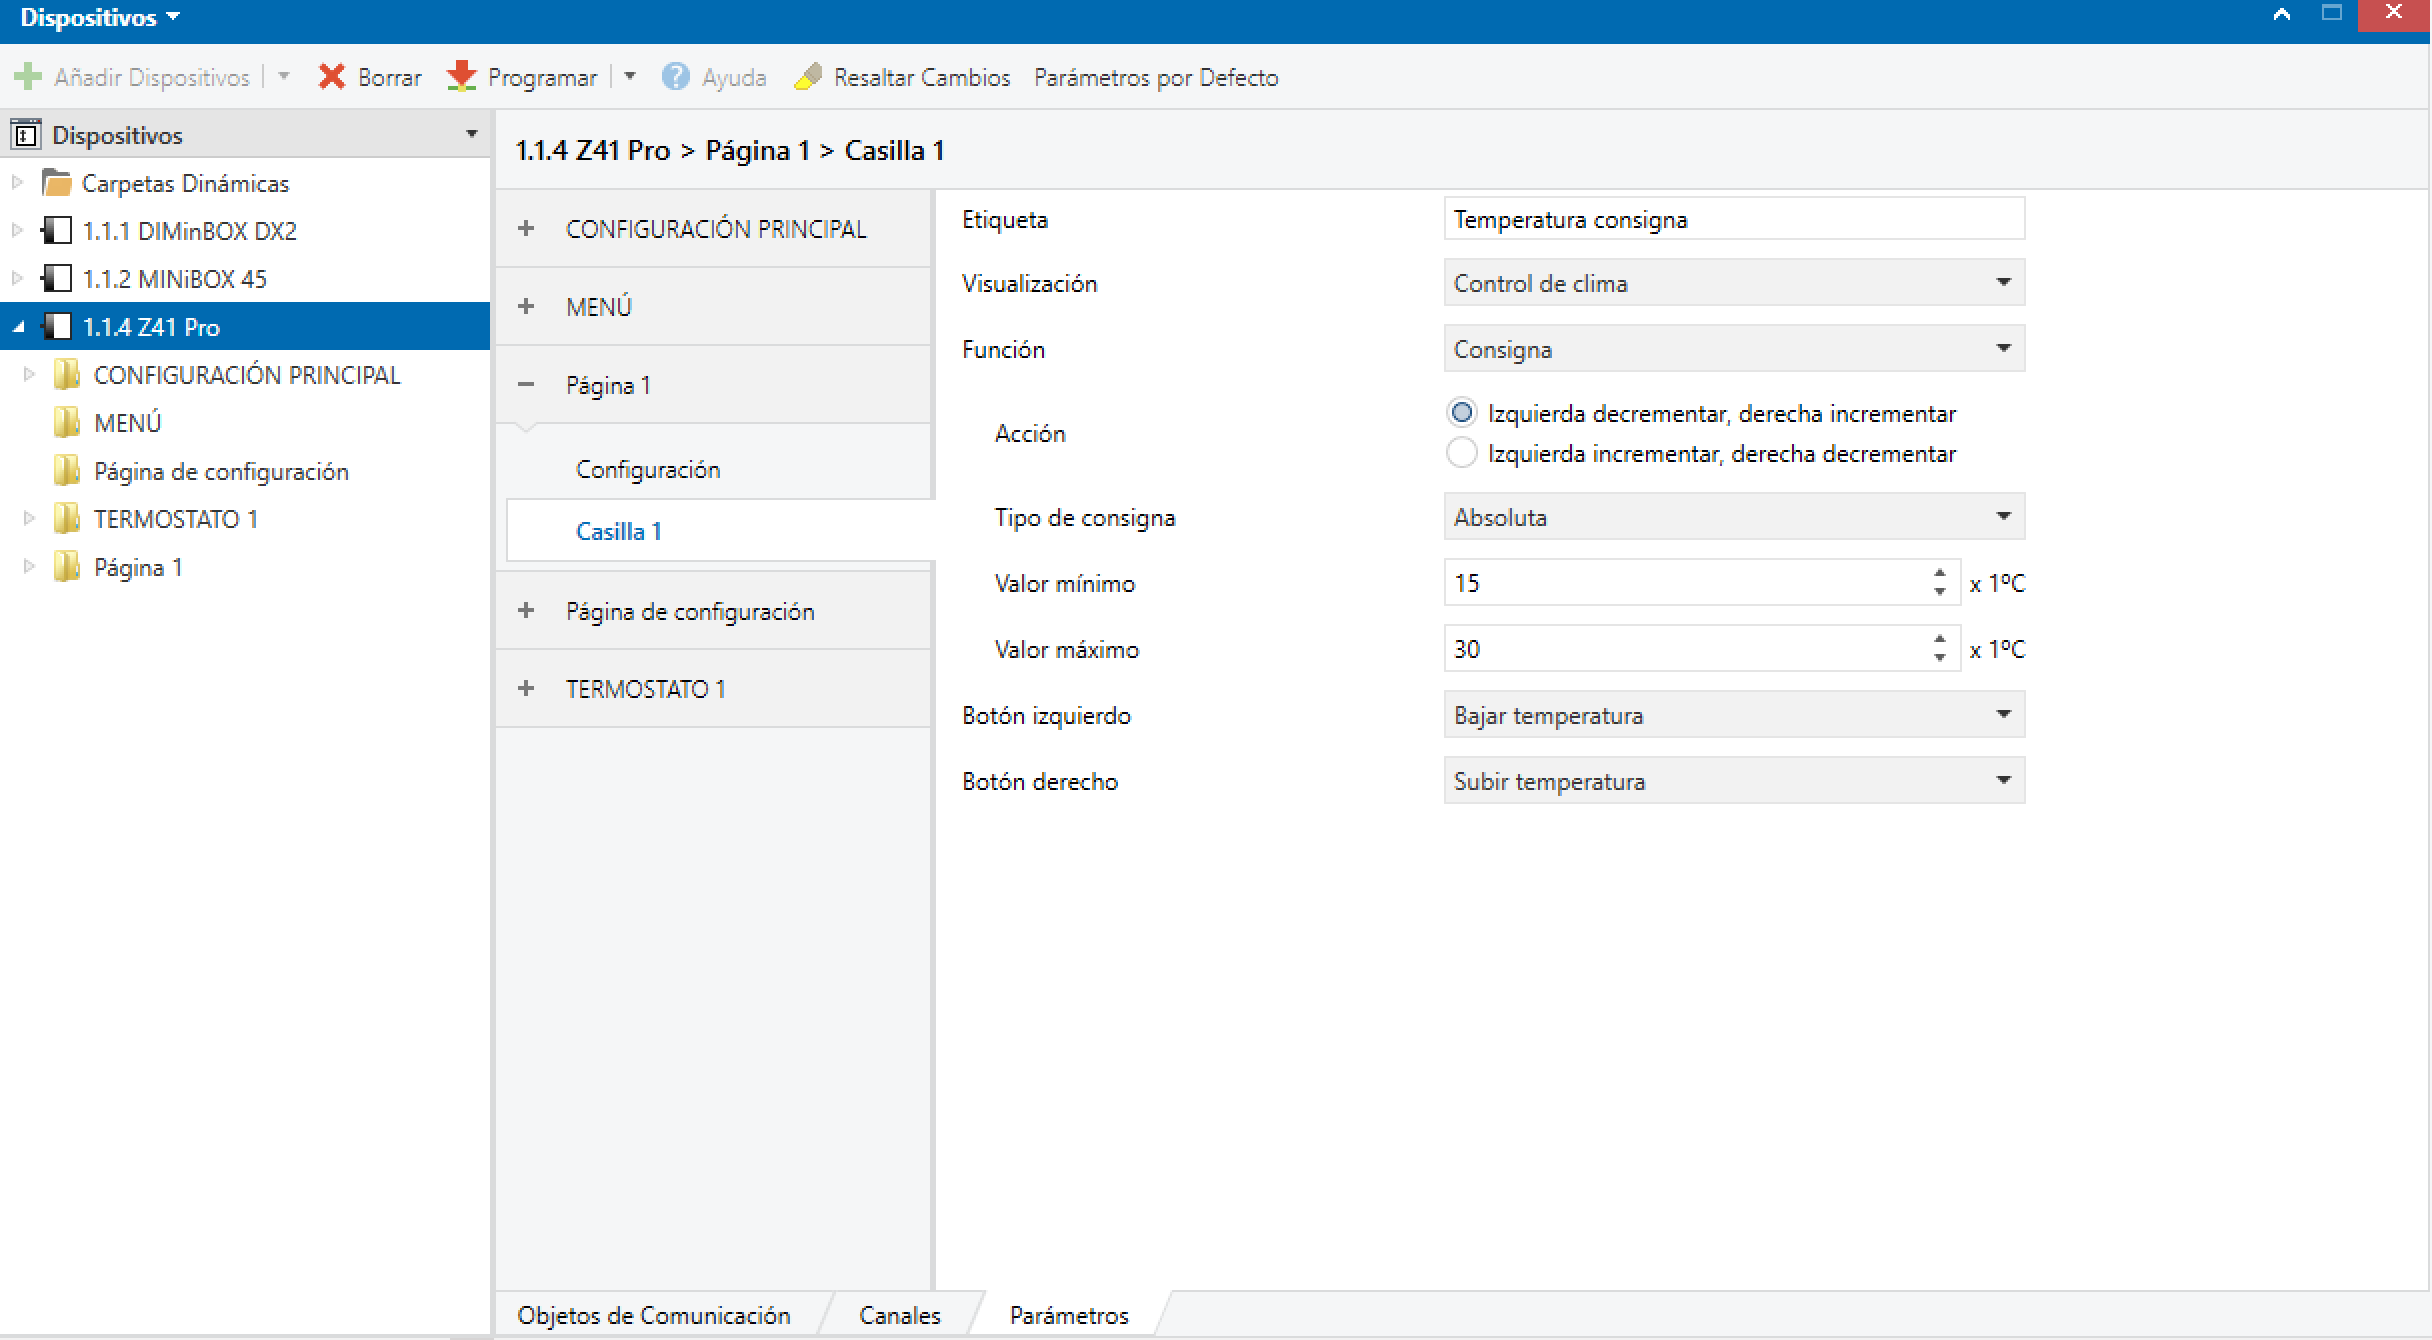
\includegraphics[width = 1.00\textwidth]{Imagenes/img27}
 		\captionof{figure}{\label{fig:IPN}Configurando dispositivo \textbf{Z41 Pro} (IV).} 
	\end{center} 
\end{figure}

Configuraremos el termostato 1 como se ha mencionado anteriormente cuya función será únicamente la de calentar cuando la temperatura se diferente a la de consigna obtenida de la fuente de temperatura 1 a través de la sonda. La consigna inicial del termostato será de 22º, siendo un grados menos la consigna para el confort. Para calentar, tanto la histéresis superior como inferior será de 0.5º. \\

\begin{figure}[H]
	\begin{center}
	 		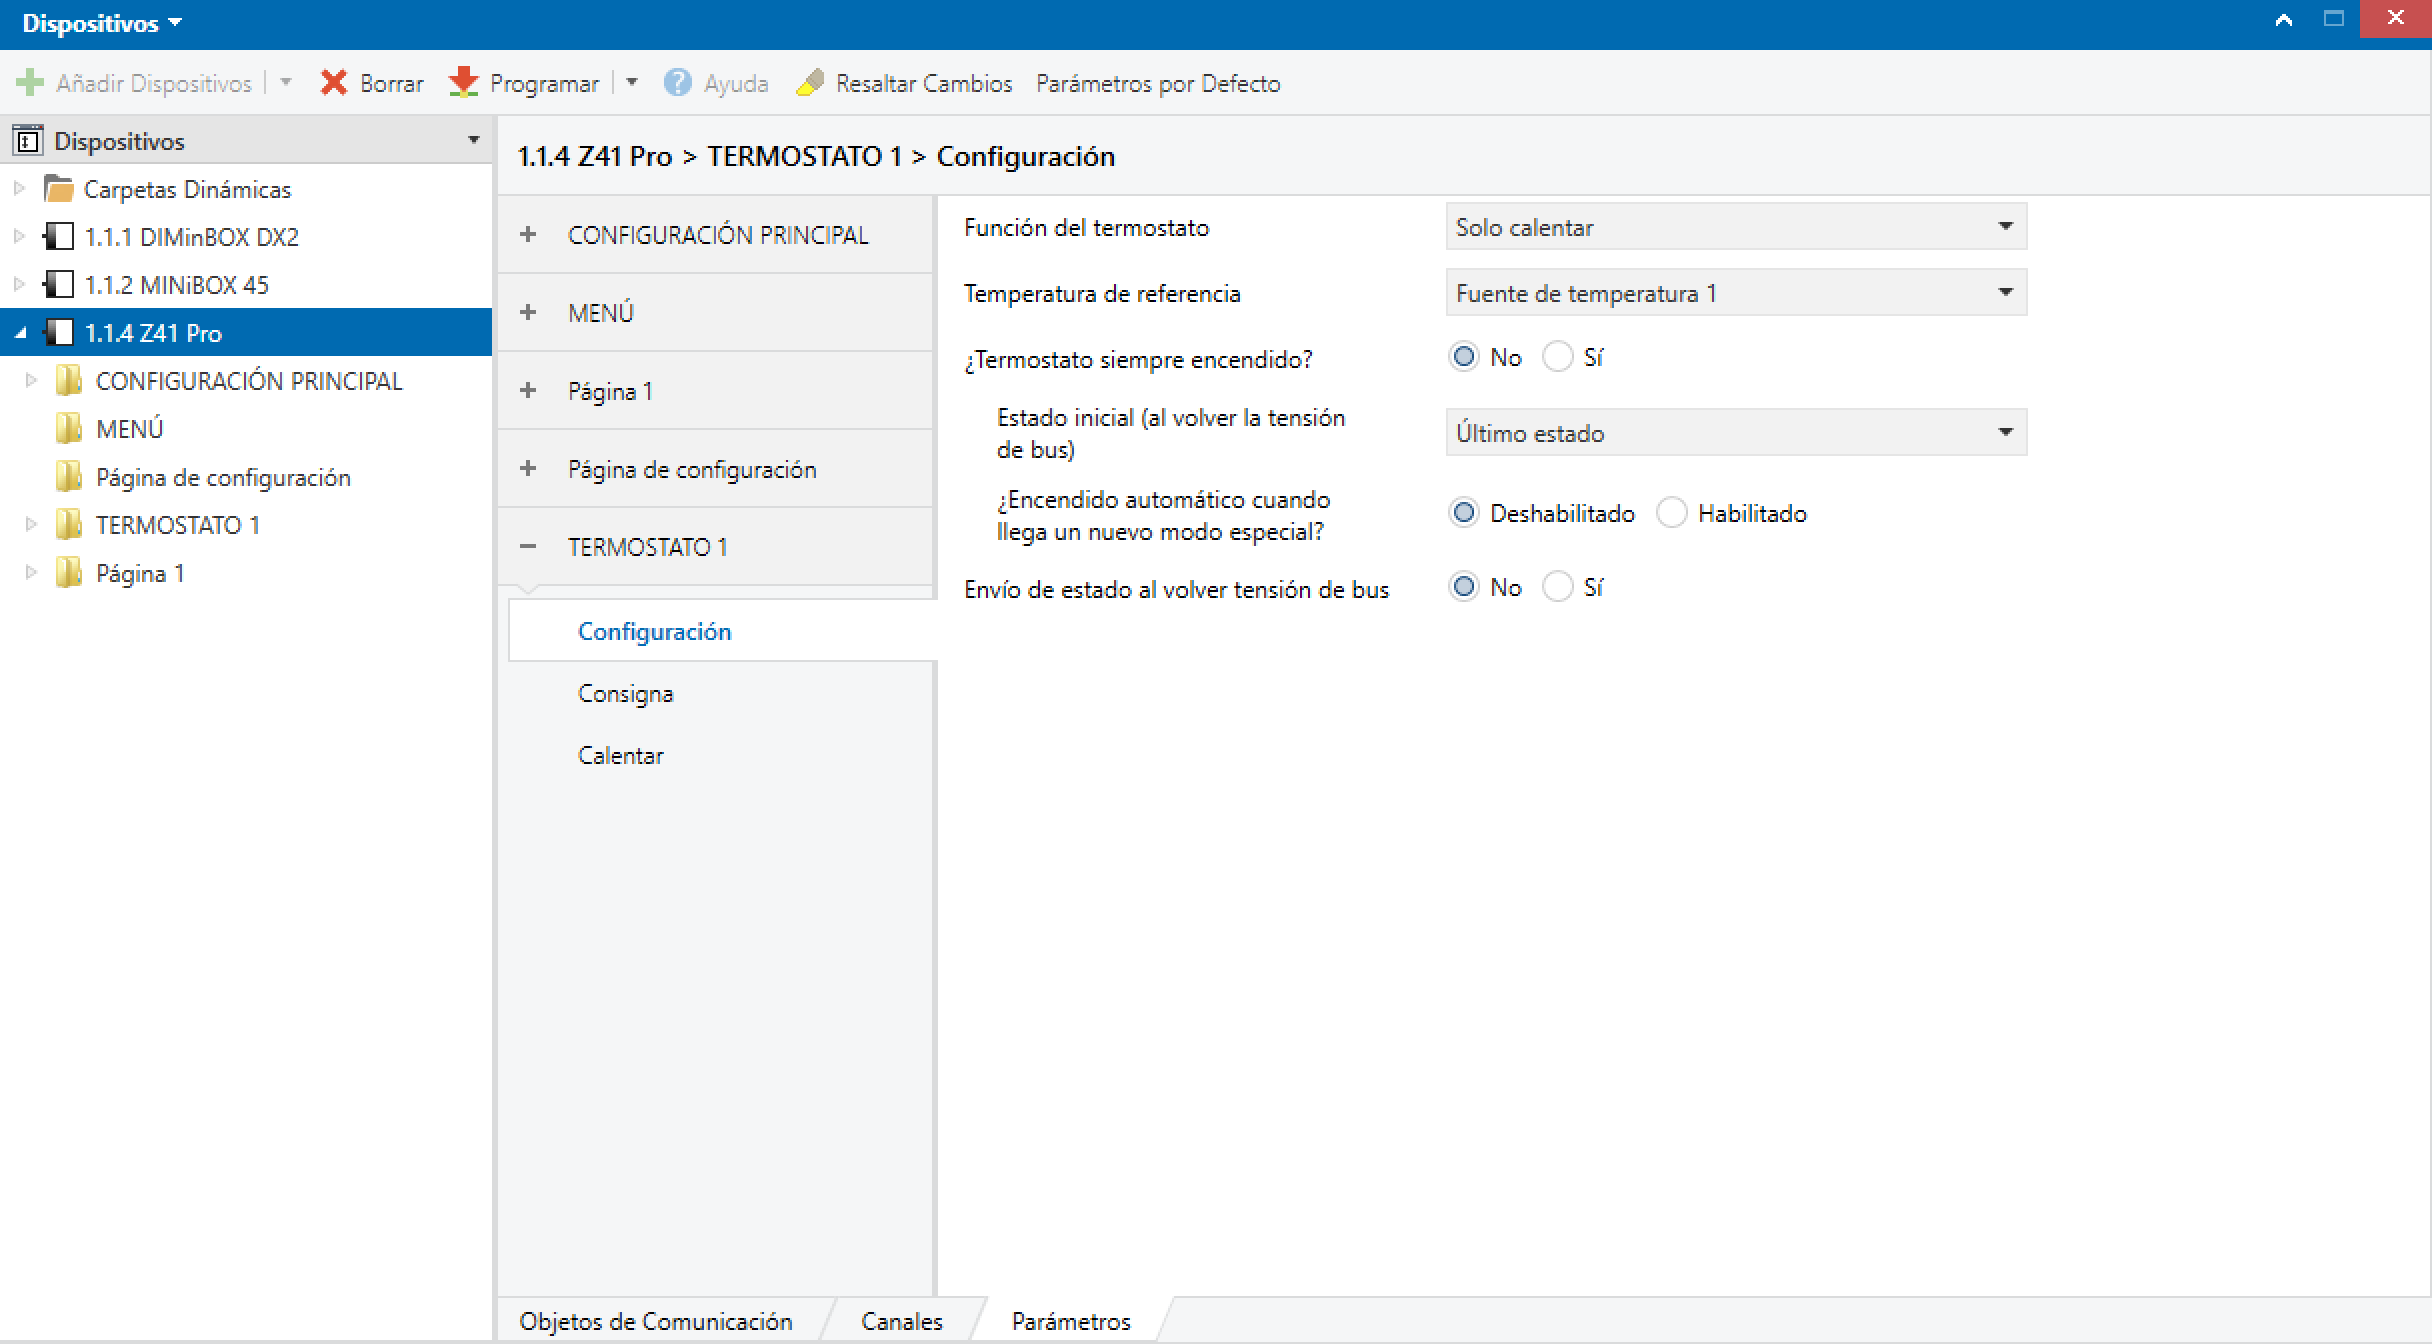
\includegraphics[width = 1.00\textwidth]{Imagenes/img28}
 		\captionof{figure}{\label{fig:IPN}Configurando termostato 1 del \textbf{Z41 Pro} (I).} 
	\end{center} 
\end{figure}

\begin{figure}[H]
	\begin{center}
	 		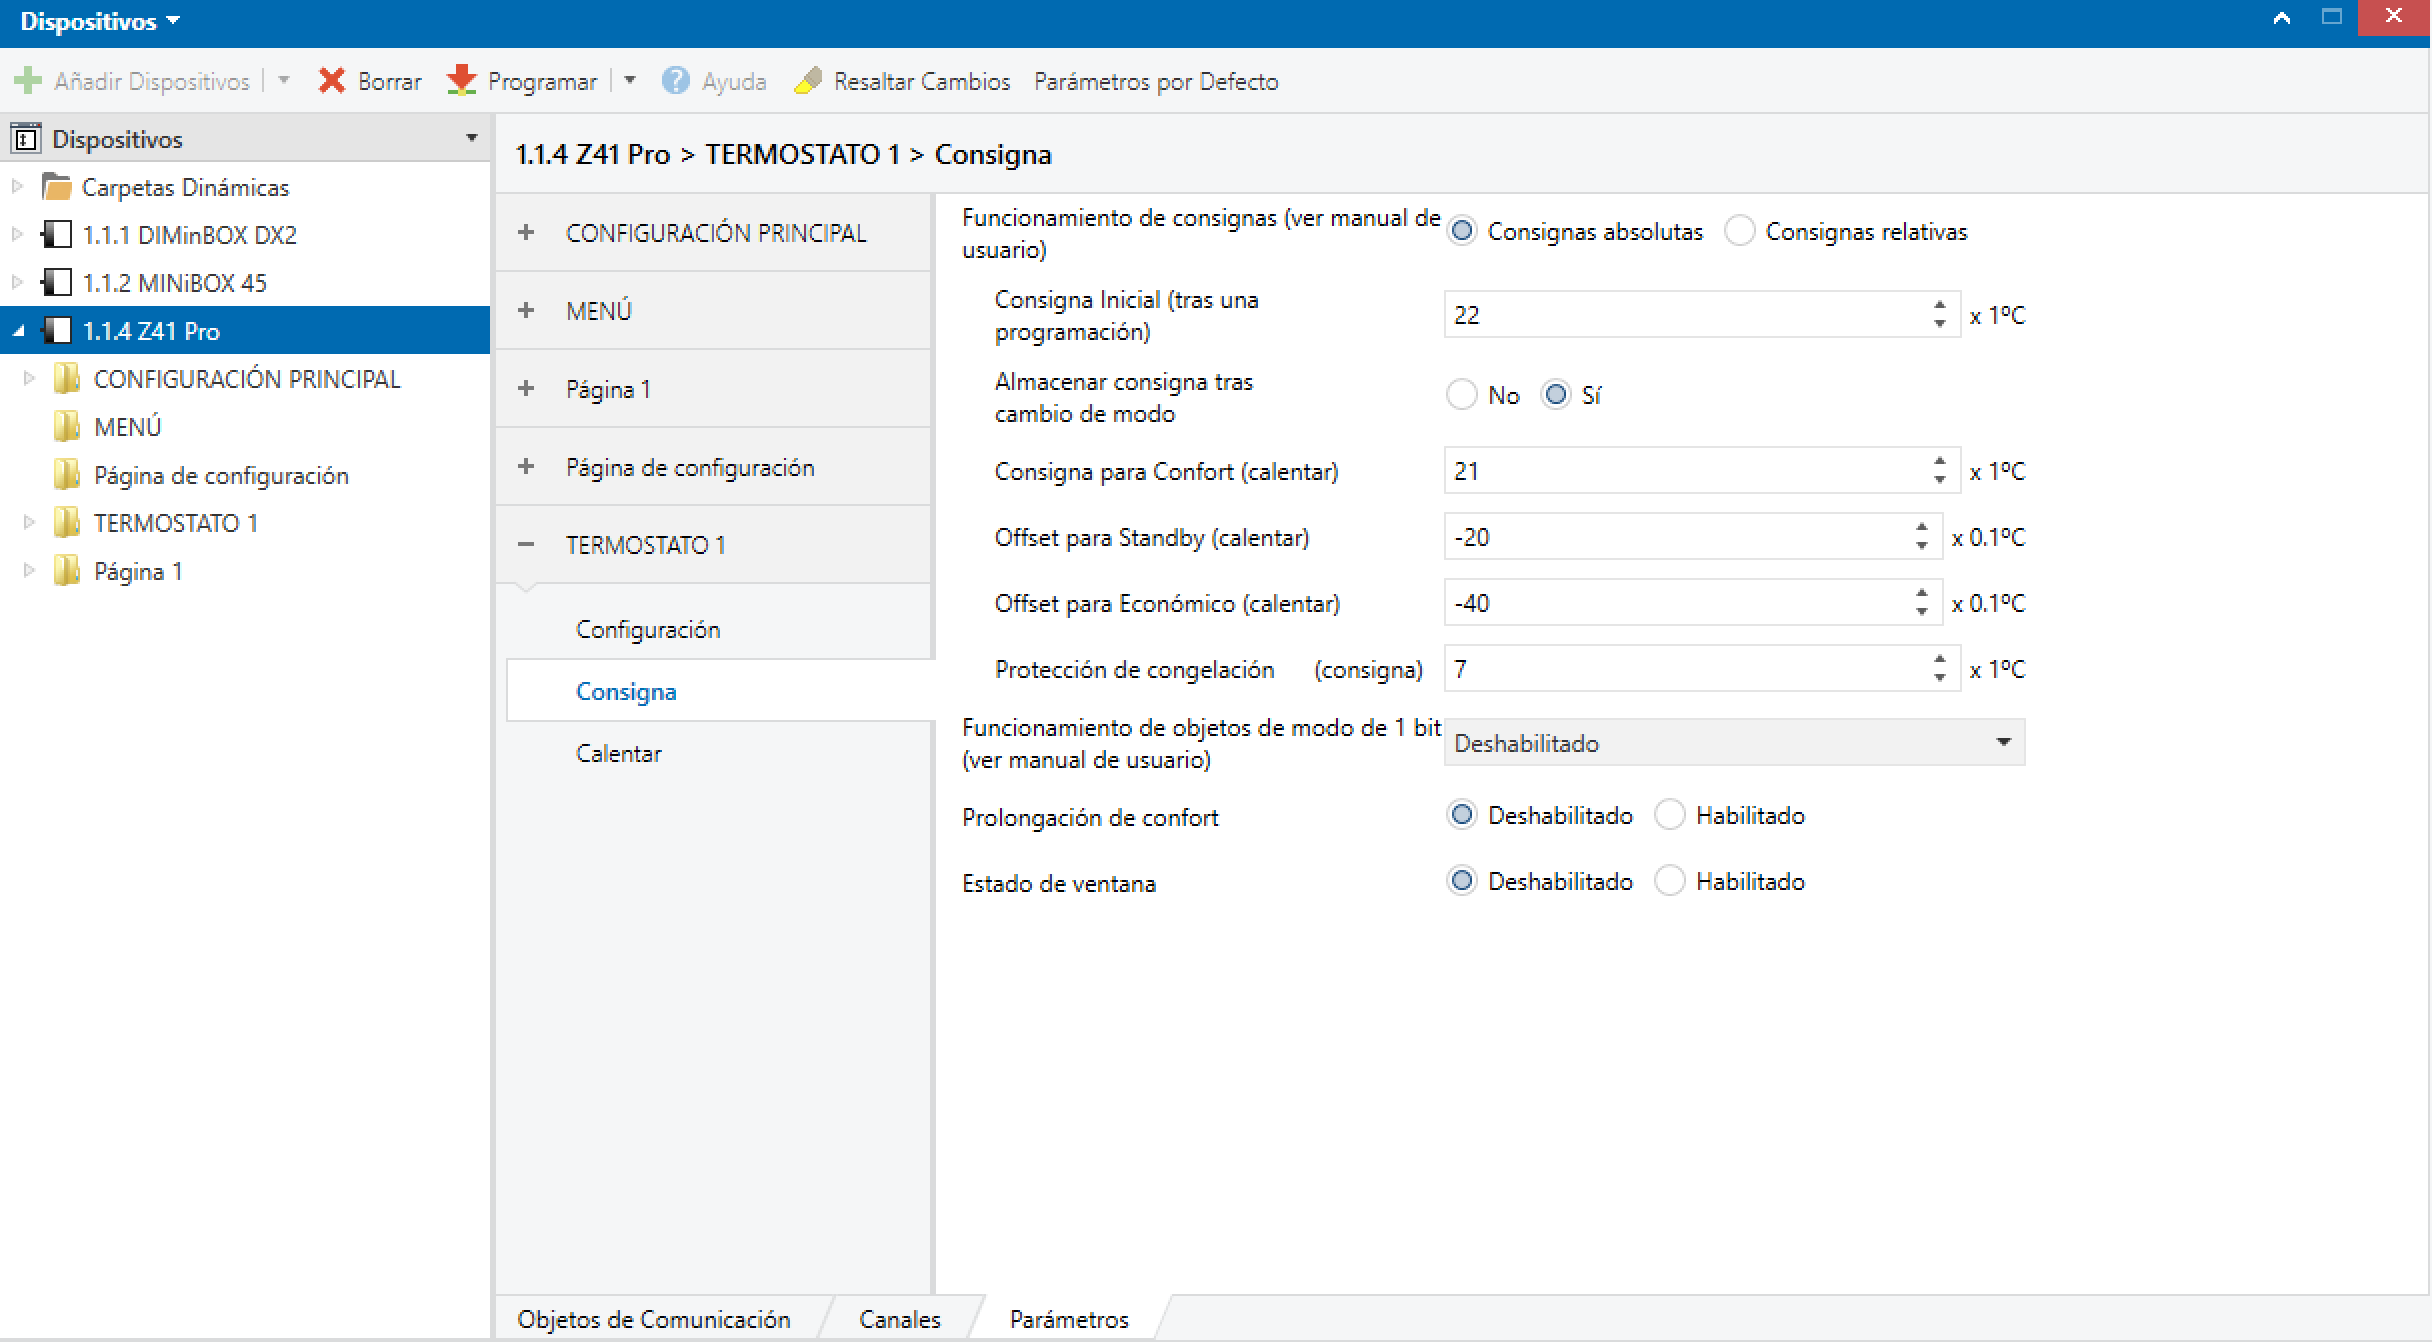
\includegraphics[width = 1.00\textwidth]{Imagenes/img29}
 		\captionof{figure}{\label{fig:IPN}Configurando termostato 1 del \textbf{Z41 Pro} (II).} 
	\end{center} 
\end{figure}

\begin{figure}[H]
	\begin{center}
	 		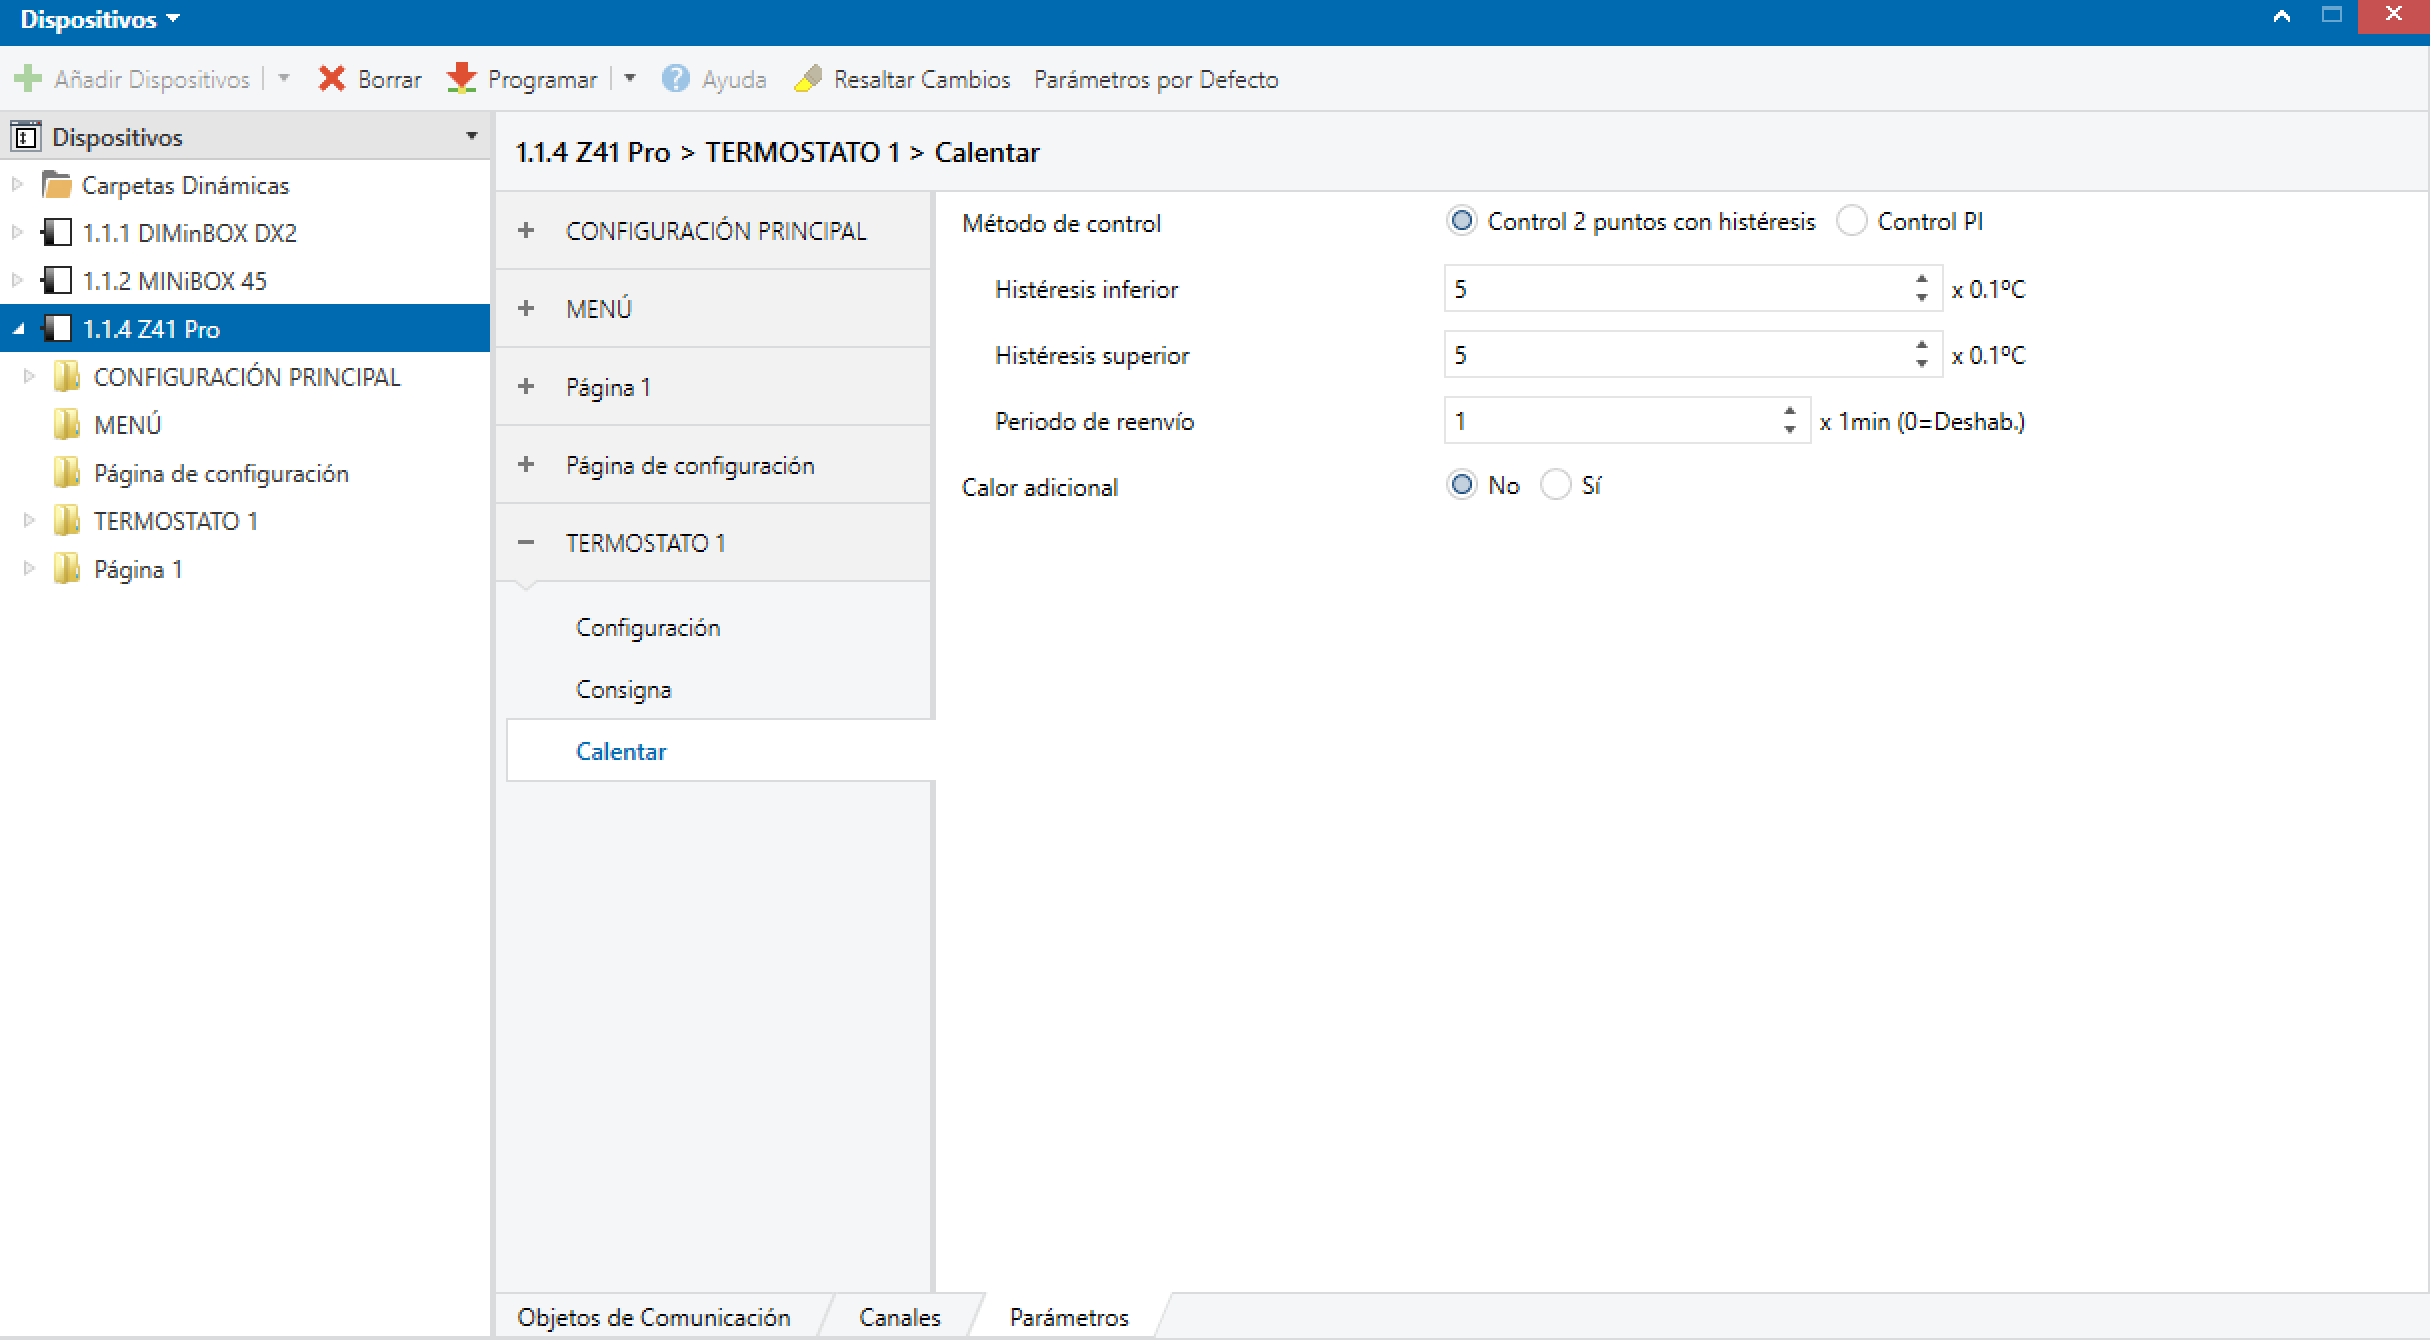
\includegraphics[width = 1.00\textwidth]{Imagenes/img30}
 		\captionof{figure}{\label{fig:IPN}Configurando termostato 1 del \textbf{Z41 Pro} (III).} 
	\end{center} 
\end{figure}

Nos crearemos tres grupos de direcciones dentro del grupo intermedio \textbf{baño}. Al grupo \textbf{temperatura\_ambiente} se le añadirán dos objetos de comunicación del dispositivo \textbf{Z41 Pro} y uno del \textbf{DIMinBox DX2}. A través de los objetos de comunicación del panel utilizaremos el [General] para mostrar la temperatura en la pantalla, y el [T1] como fuente de temperatura 1que lo que hará será medir el sensor externo. Del dispositivo \textbf{DIMinBox DX2} añadiremos la entrada 1 como objeto de comunicación para obtener el valor del sensor de temperatura, es decir, la temperatura acual. \\

\begin{figure}[H]
	\begin{center}
	 		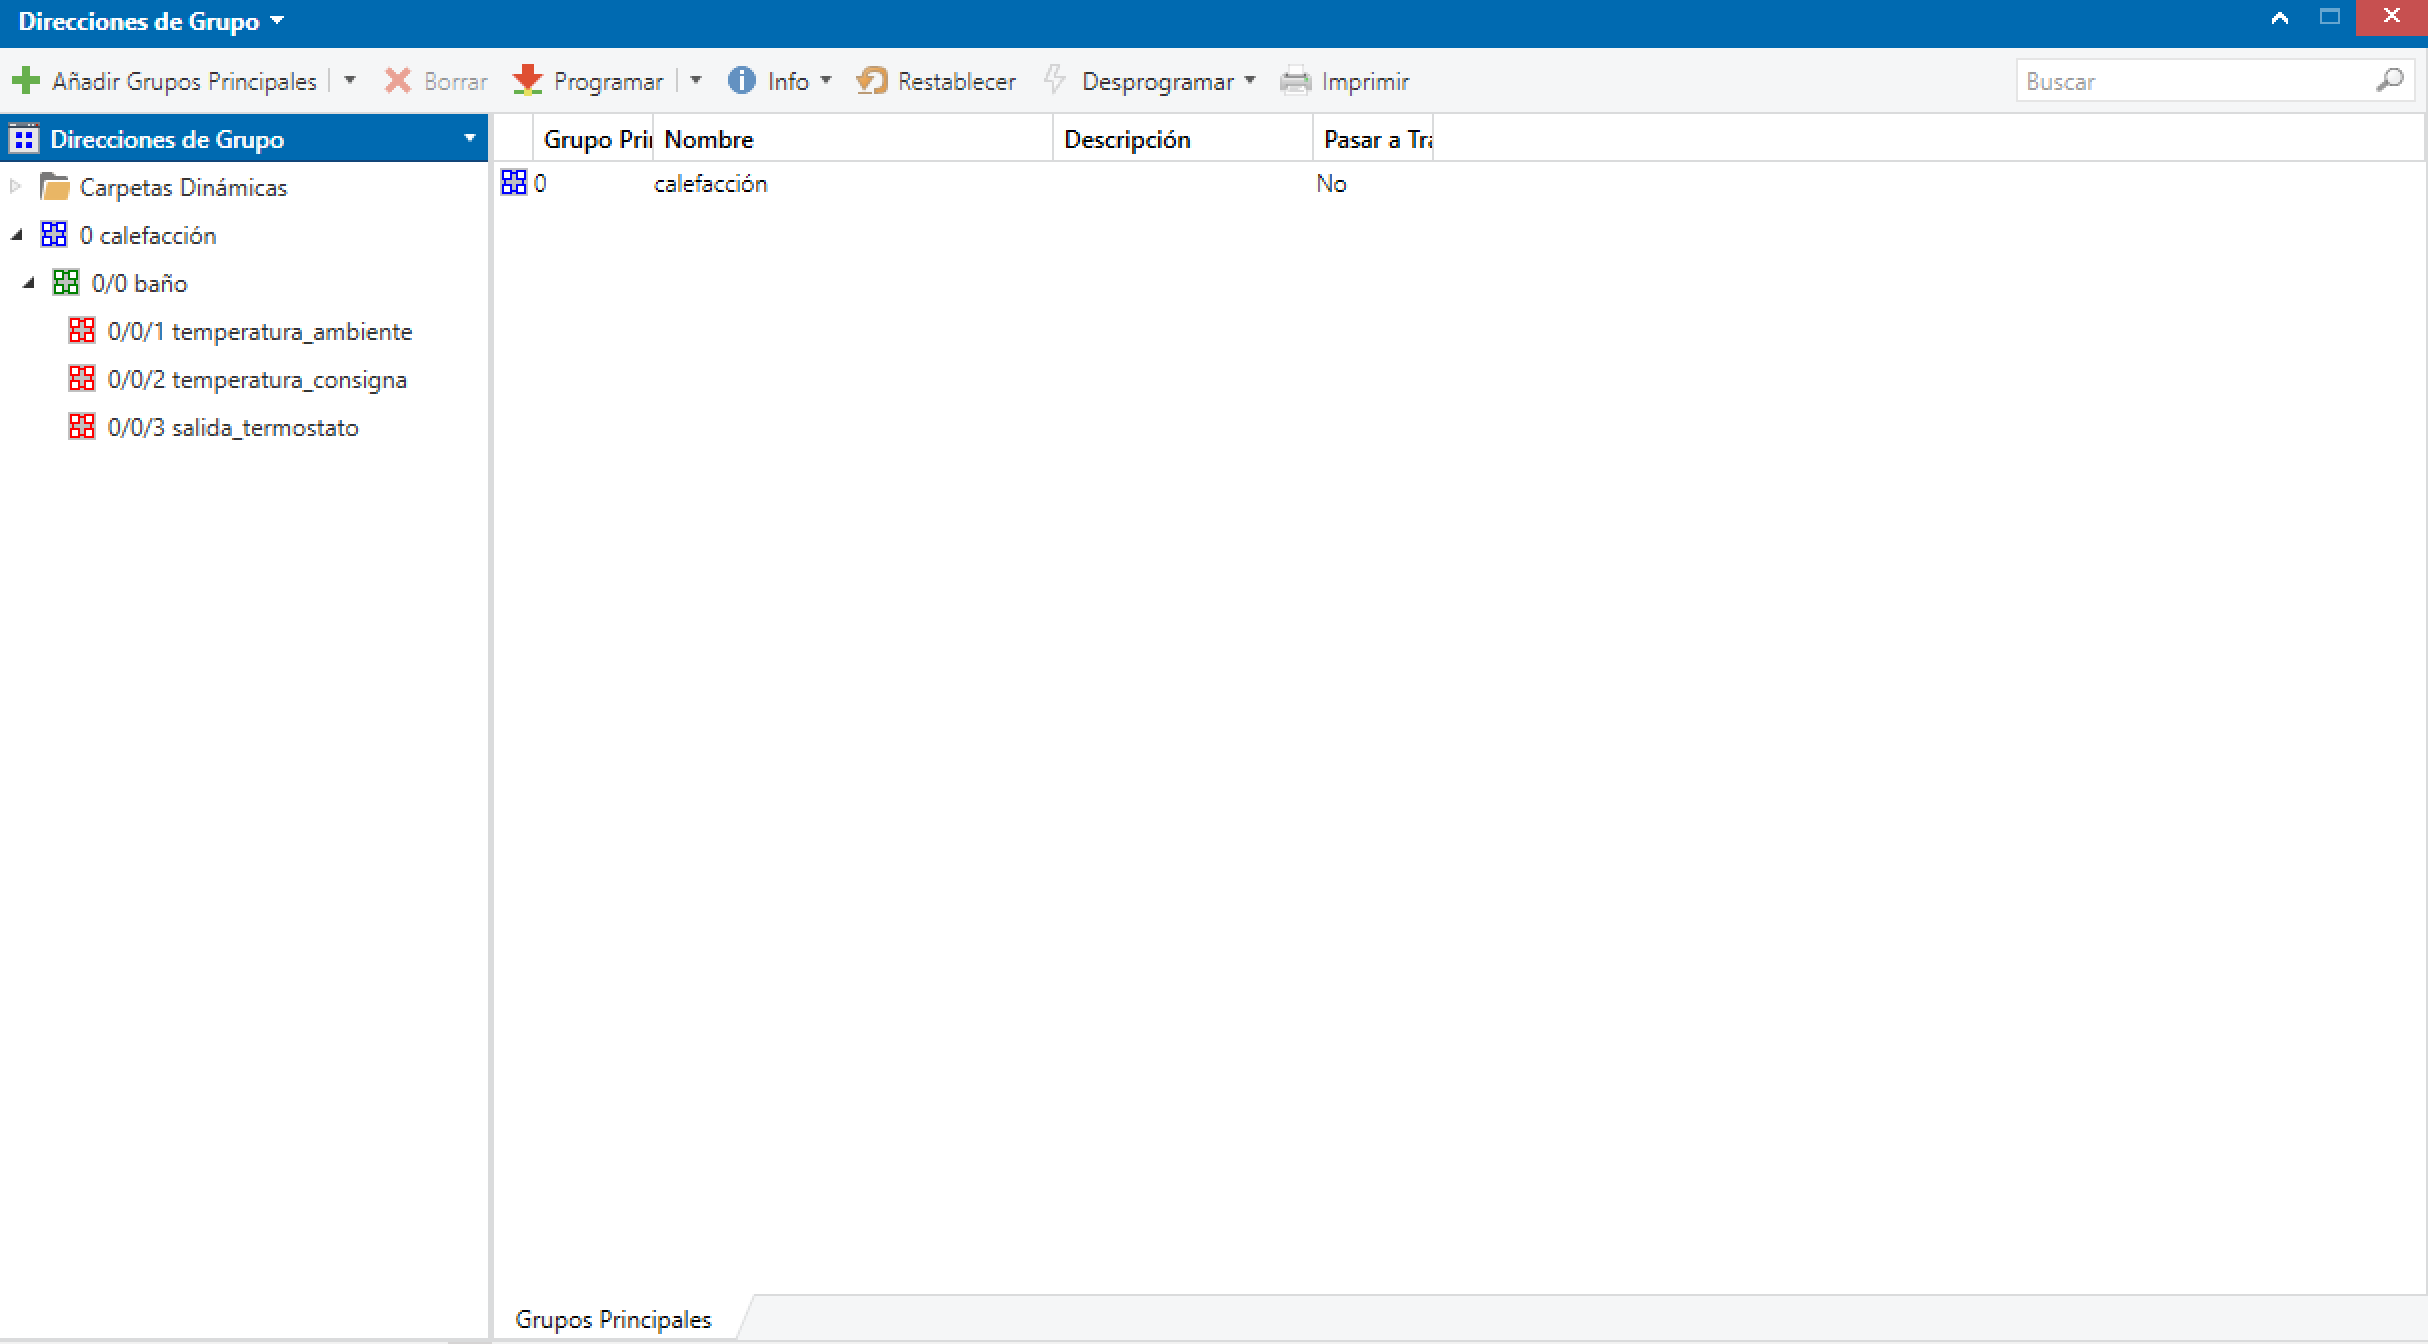
\includegraphics[width = 1.00\textwidth]{Imagenes/img31}
 		\captionof{figure}{\label{fig:IPN}Agregando direcciones de grupo.} 
	\end{center} 
\end{figure}

\begin{figure}[H]
	\begin{center}
	 		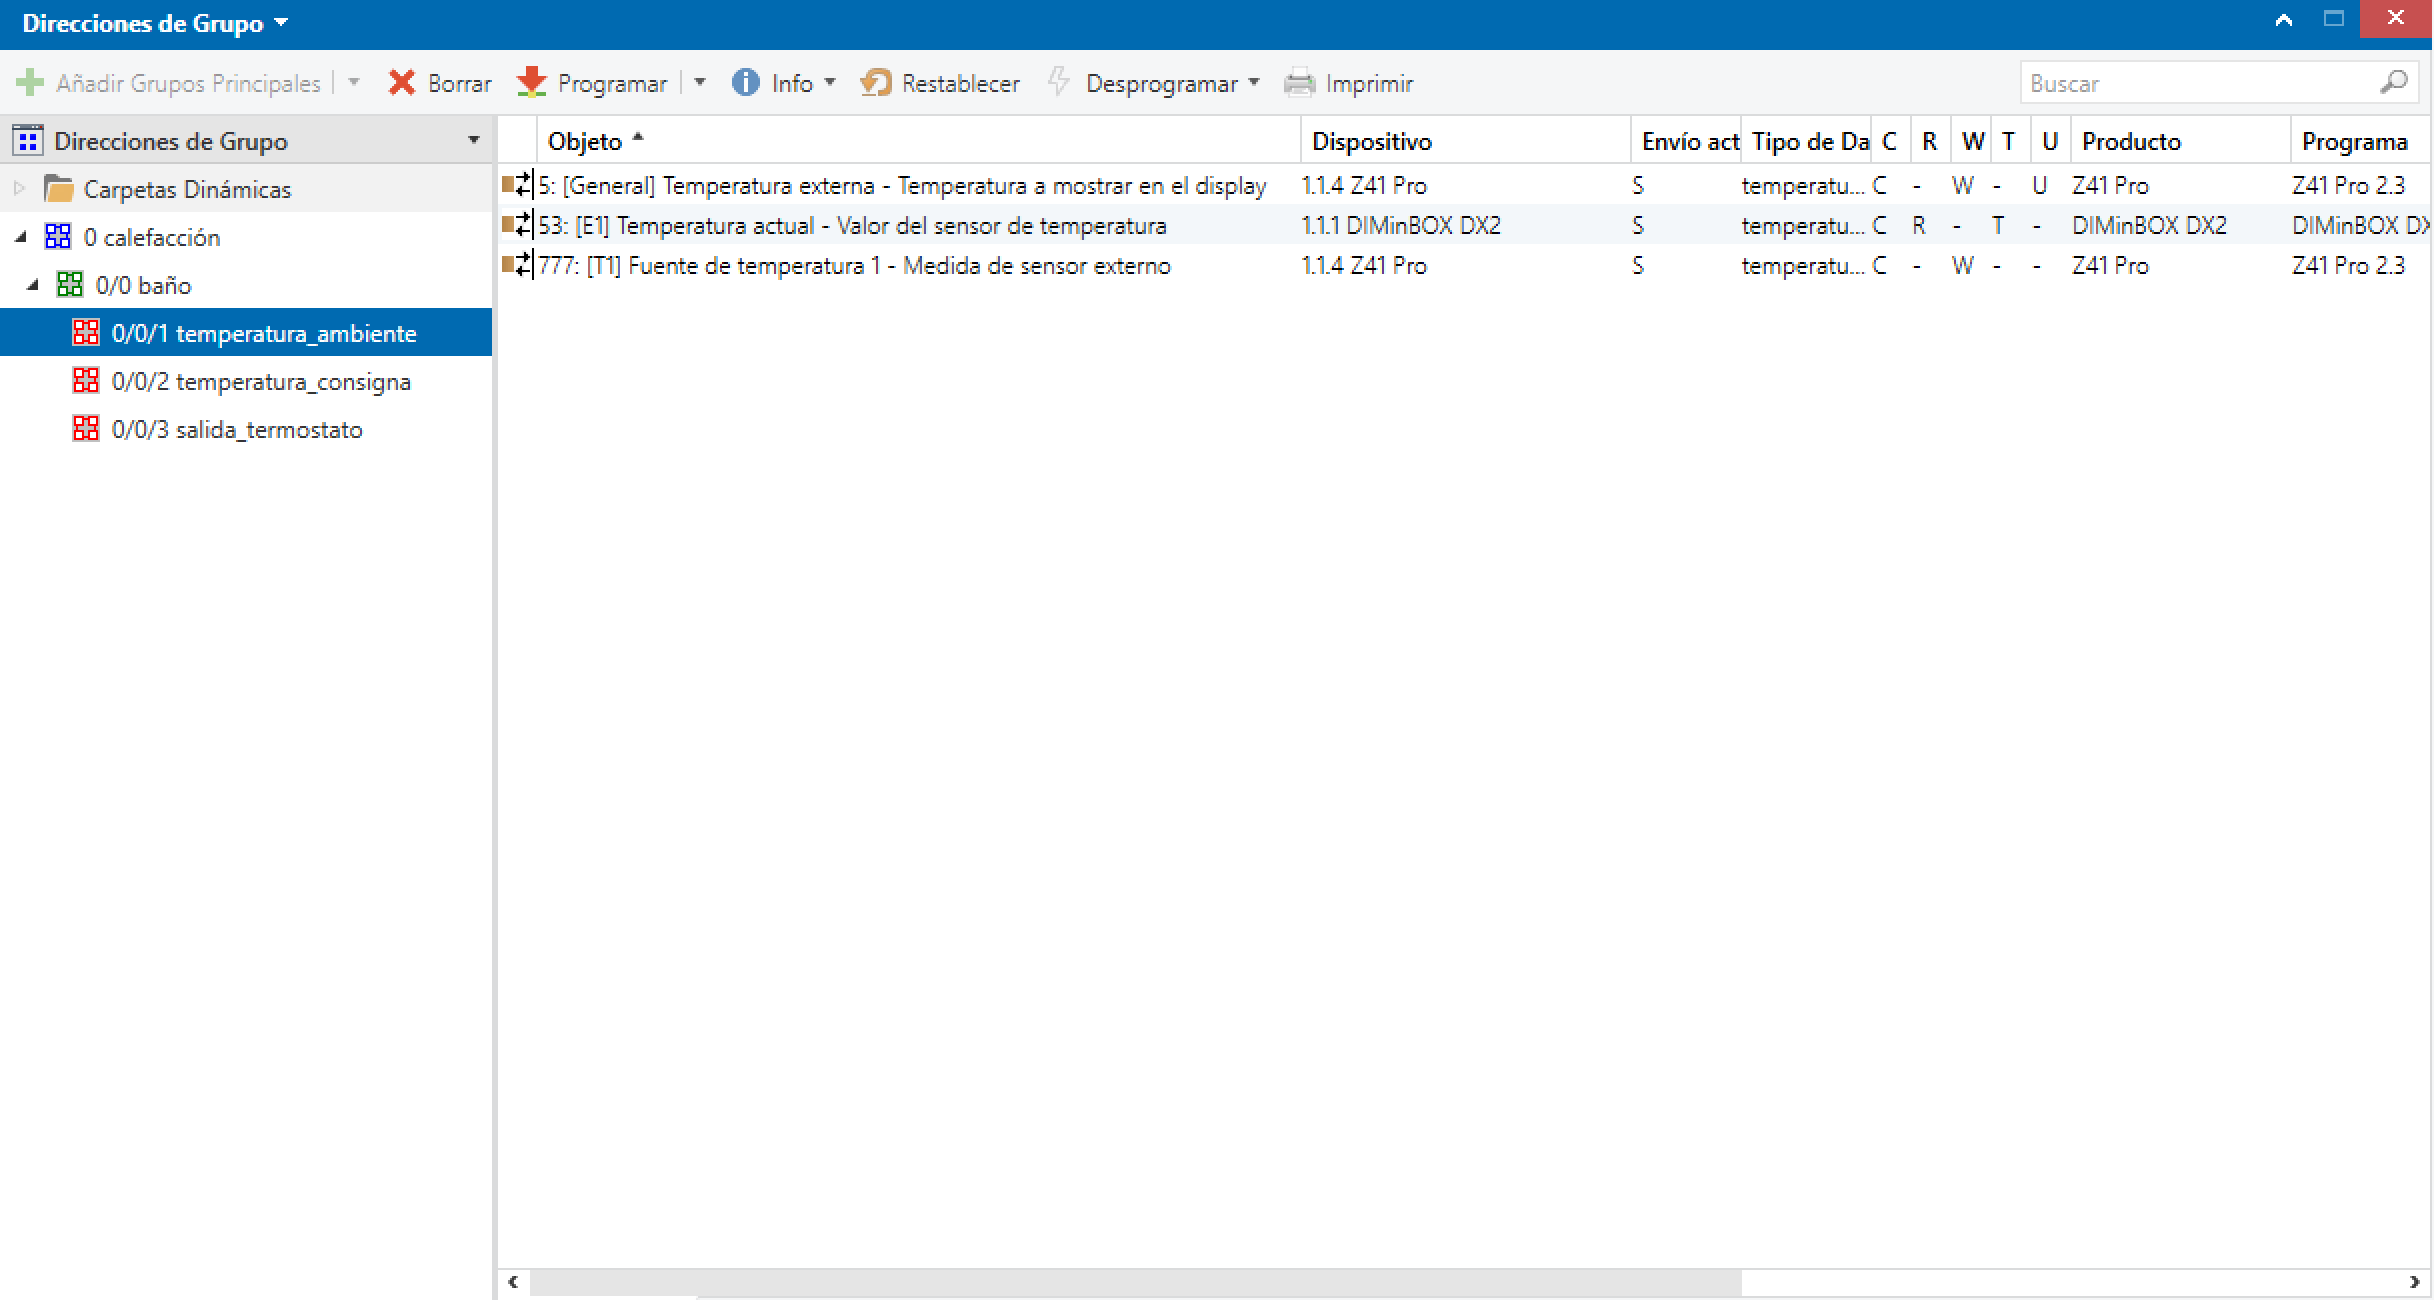
\includegraphics[width = 1.00\textwidth]{Imagenes/img32}
 		\captionof{figure}{\label{fig:IPN}Añadiendo objetos de comunicación a la dirección de grupo \textbf{temperatura\_ambiente}.} 
	\end{center} 
\end{figure}

El grupo de direcciones \textbf{temperatura\_consigna} sólo incluirá objetos de comunicación del dispositivo \textbf{Z41 Pro}. El objeto [P1][B1] para el control de la temperatura (el valor absoluto en coma flotante) y el objeto consigna [T1] para la consigna del temostato. \\

\begin{figure}[H]
	\begin{center}
	 		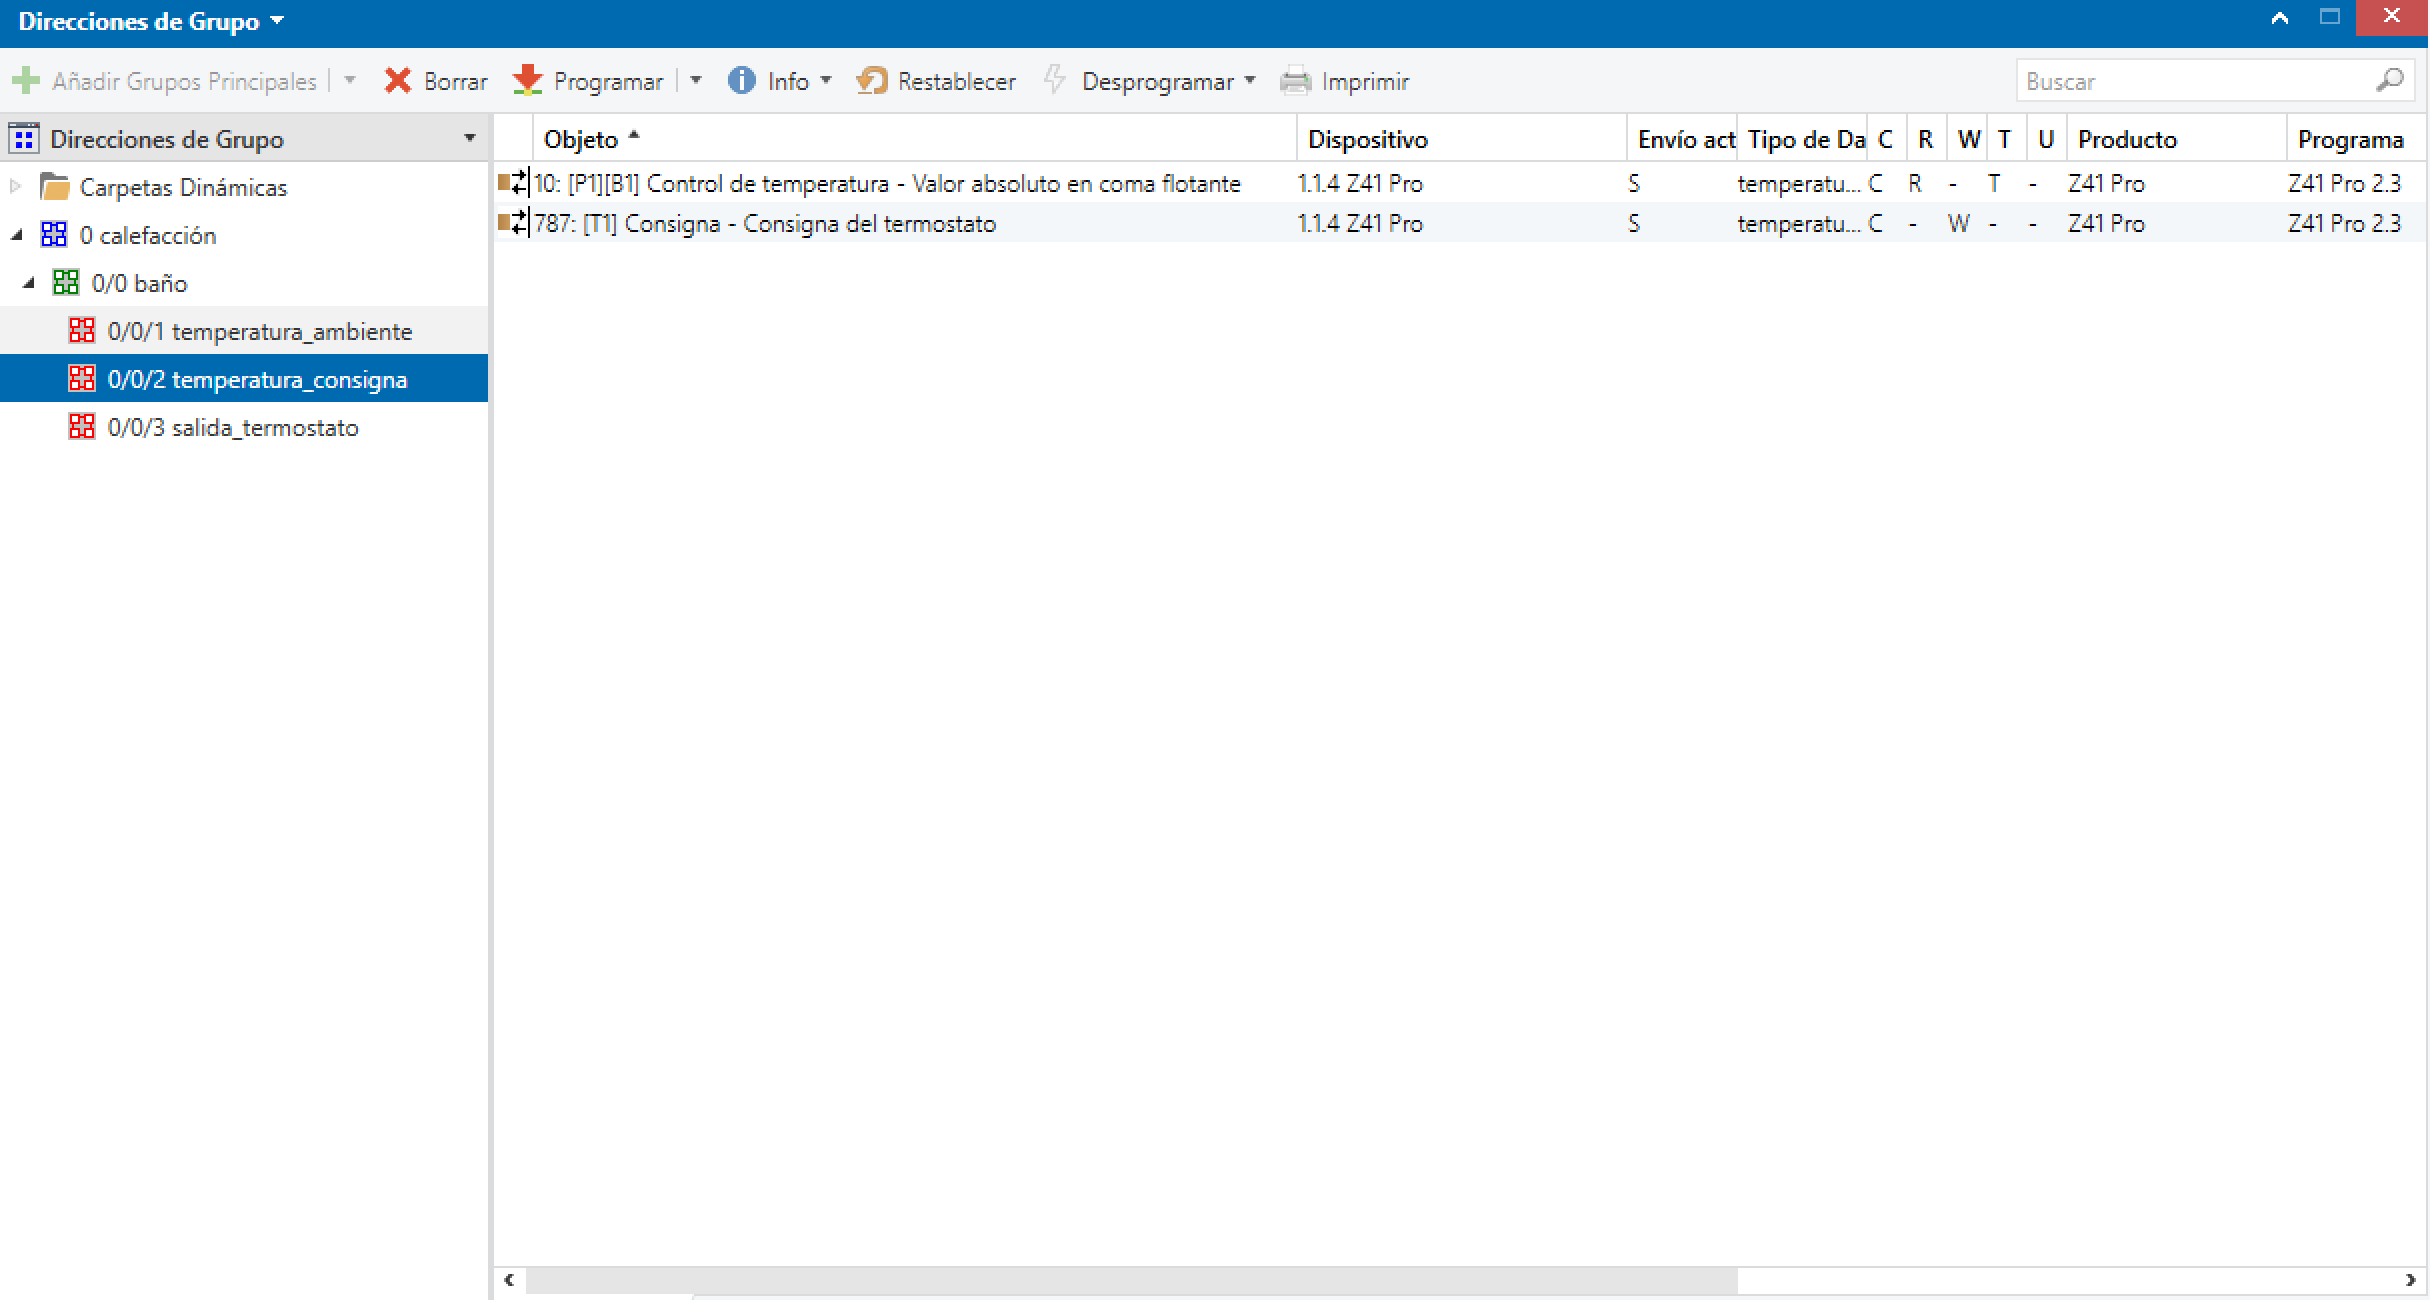
\includegraphics[width = 1.00\textwidth]{Imagenes/img33}
 		\captionof{figure}{\label{fig:IPN}Añadiendo objetos de comunicación a la dirección de grupo \textbf{temperatura\_consigna}.} 
	\end{center} 
\end{figure}

El último grupo de direcciones (\textbf{salida\_termostato}) tendrá un objeto de comunicación del \textbf{MINinBOX 45} para apagar o encender el relé para calentar o no calentar el baño (\textbf{S3}) y un objeto de comunicación del \textbf{Z41 Pro} como variable de control para calentar (\textbf{T1}).\\ 

\begin{figure}[H]
	\begin{center}
	 		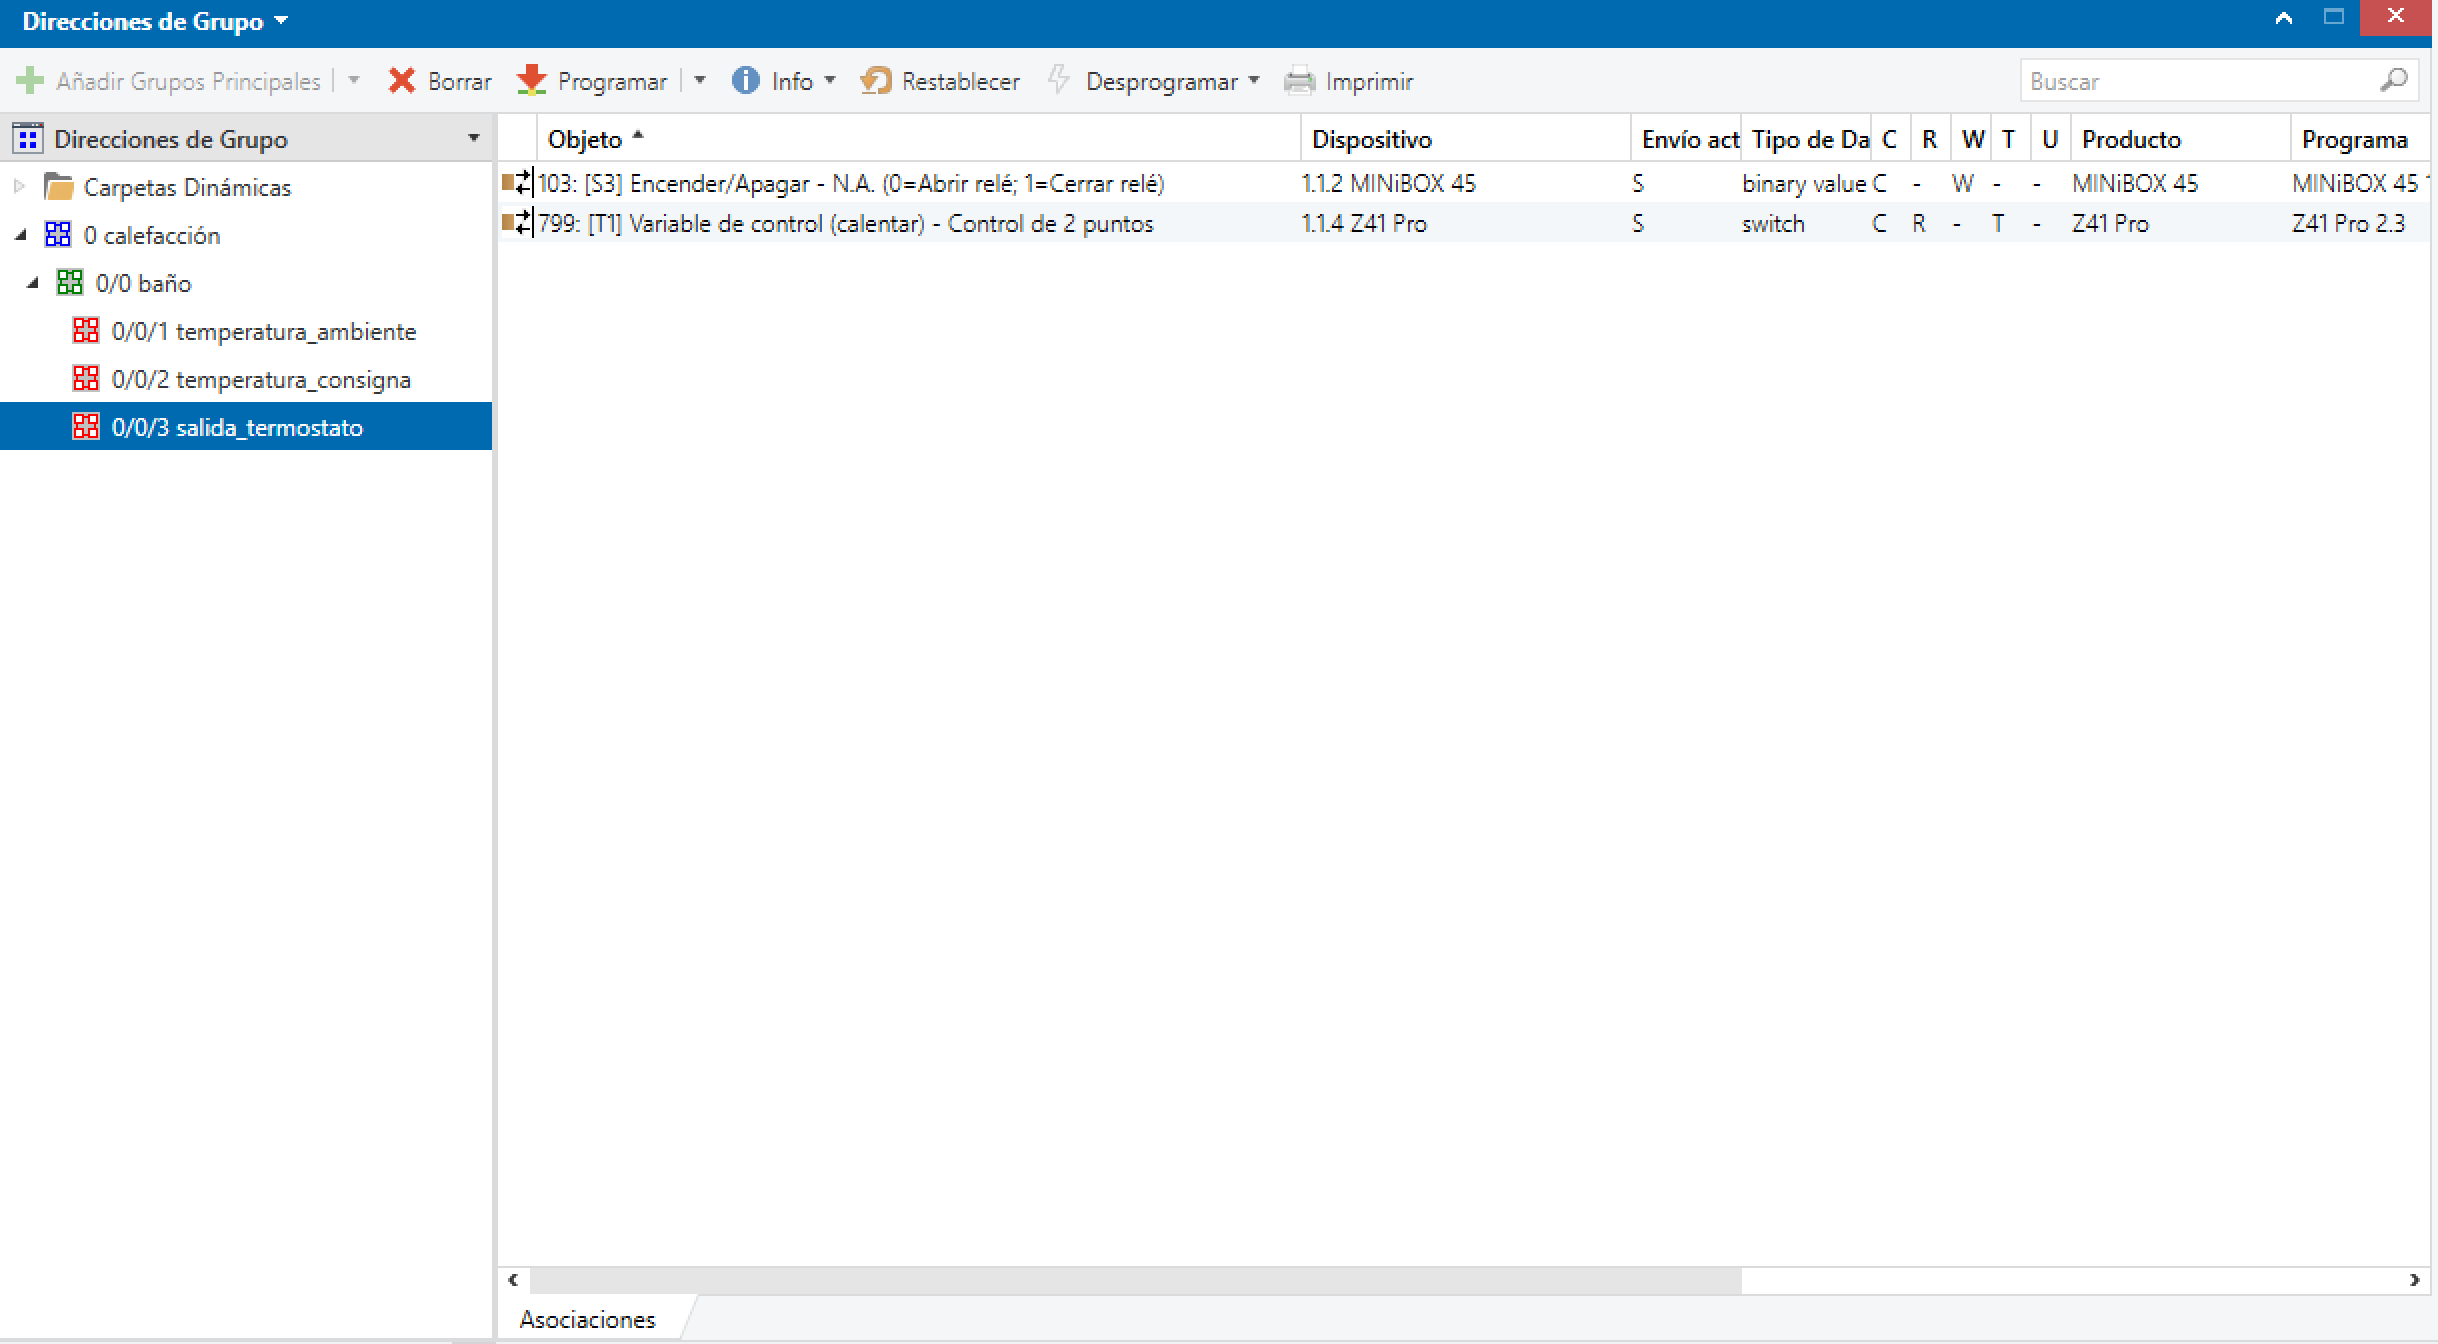
\includegraphics[width = 1.00\textwidth]{Imagenes/img34}
 		\captionof{figure}{\label{fig:IPN}Añadiendo objetos de comunicación a la dirección de grupo \textbf{salida\_termostato}.} 
	\end{center} 
\end{figure}

Ya podemos enviarlos a programar para ver su correcto funcionamiento como se hizo en clase. \\


\section{Práctica 4. Control de persianas.} 
Se va configurar KNX para realizar el control de unas persianas. El supuesto consiste en mover o parar unas persianas presionando un botón del teclado para lo que será necesario utilizar los dispositivos \textbf{Touch-MyDesing Plus 6} para el control de los botones y \textbf{MINiBOX 45} para activar o desactivar el relé que movería las persianas. \\

\begin{figure}[H]
	\begin{center}
	 		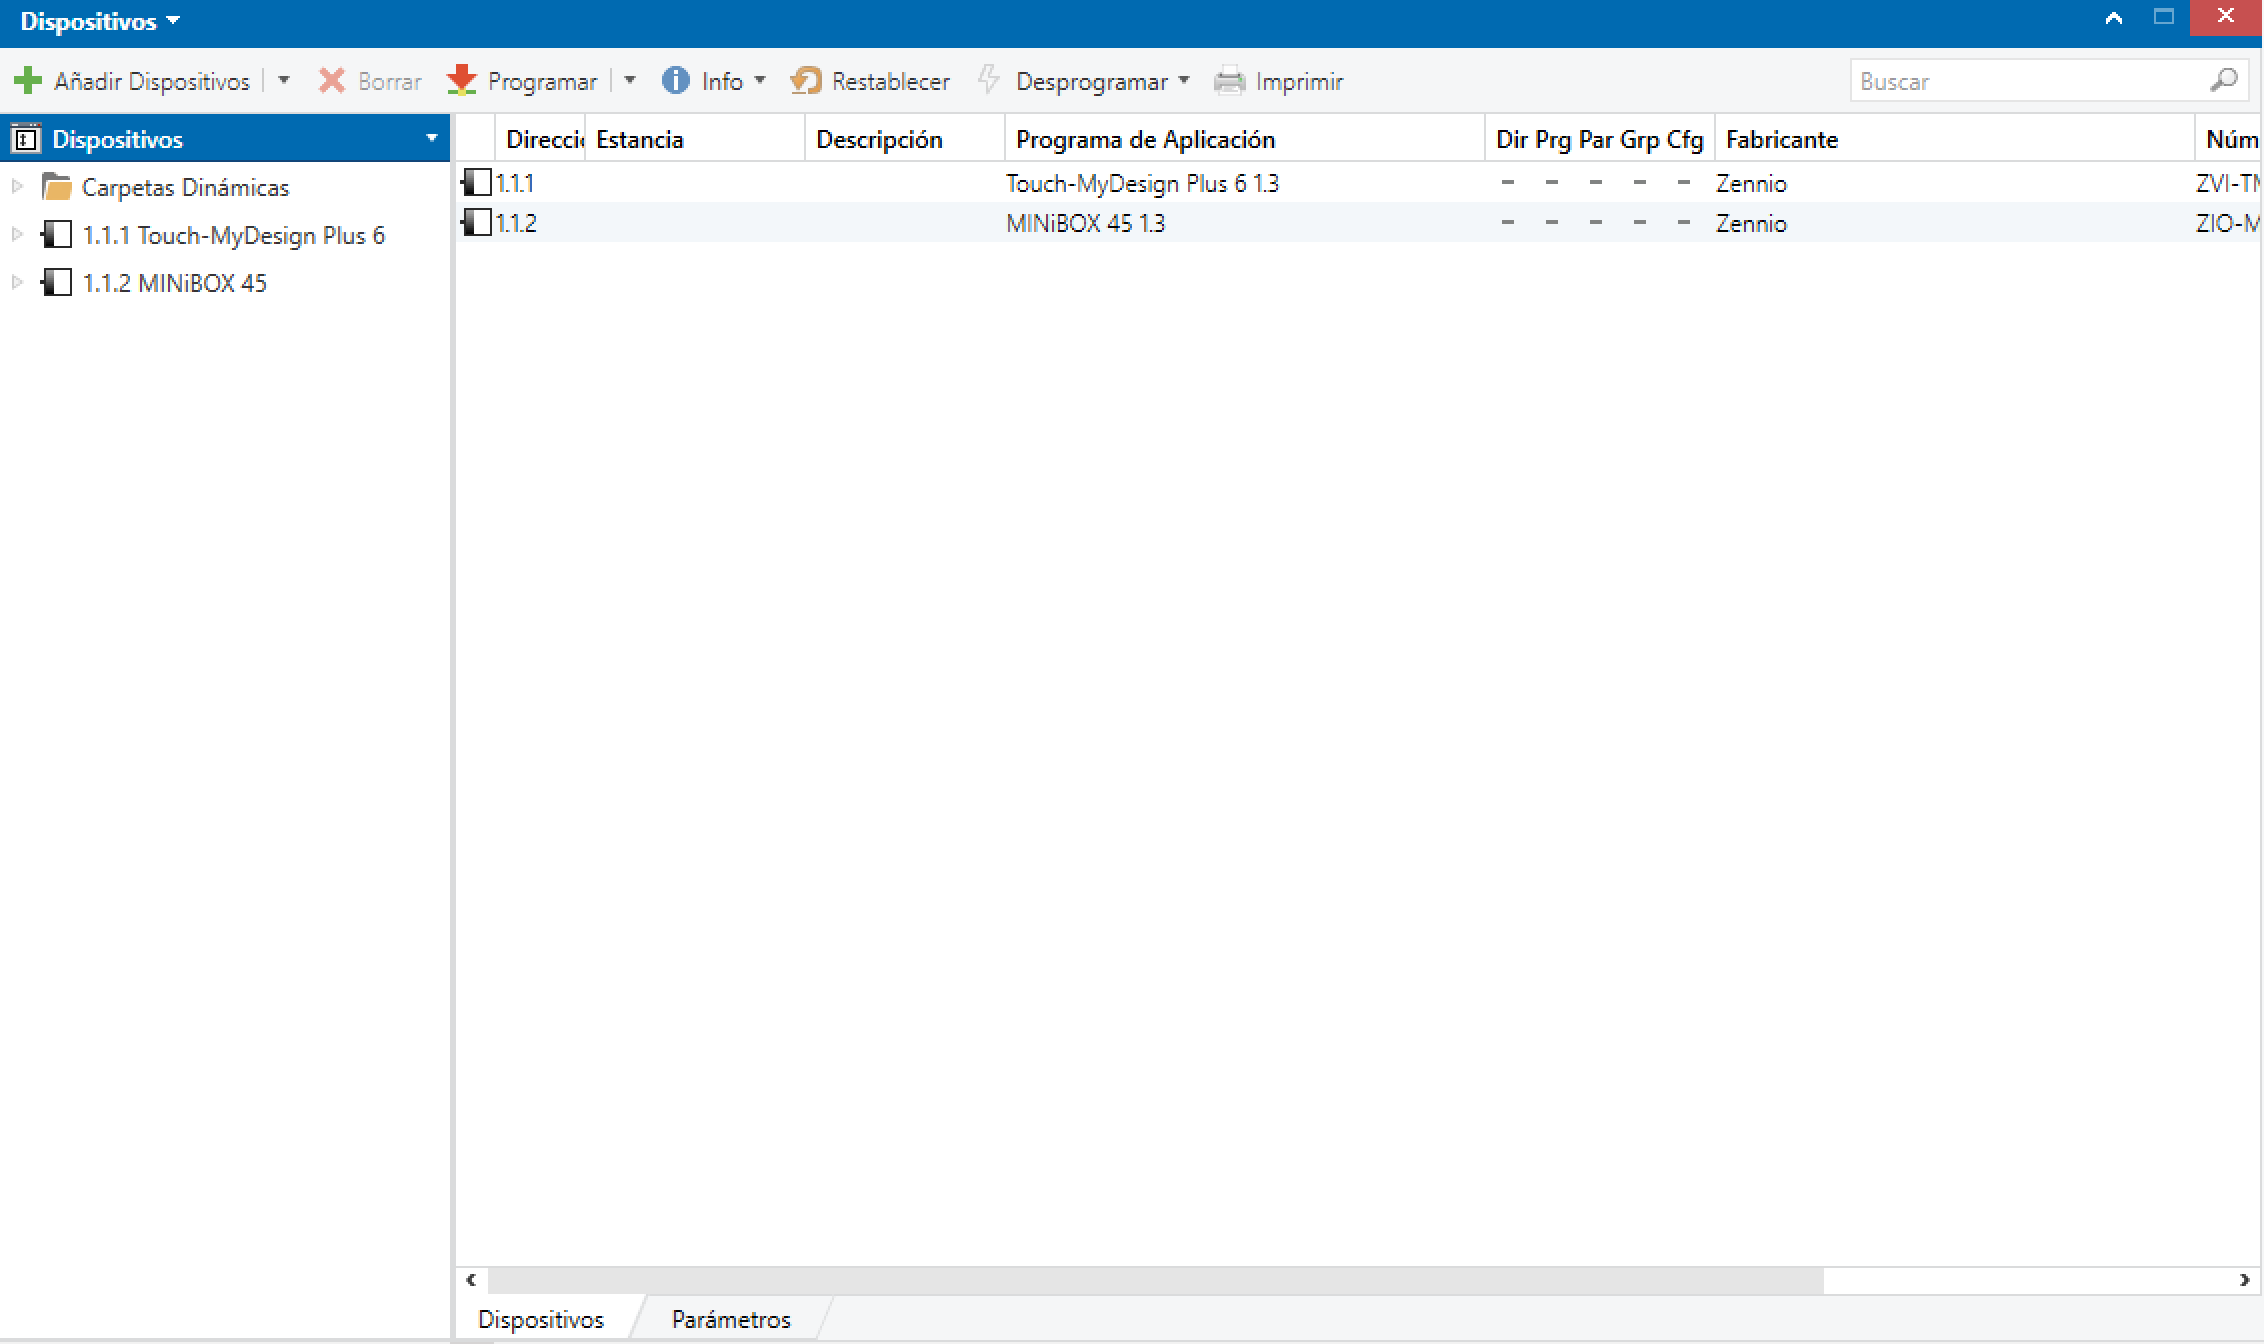
\includegraphics[width = 1.00\textwidth]{Imagenes/img35}
 		\captionof{figure}{\label{fig:IPN}Agregando dispositivos.} 
	\end{center} 
\end{figure}

Comenzaremos configurando el panel \textbf{Touch-MyDesing Plus 6} habilitando la pareja C de pulsadores principales. A dicha pareja se le establecerá la función de persianas y de tipo estándar. \\

\begin{figure}[H]
	\begin{center}
	 		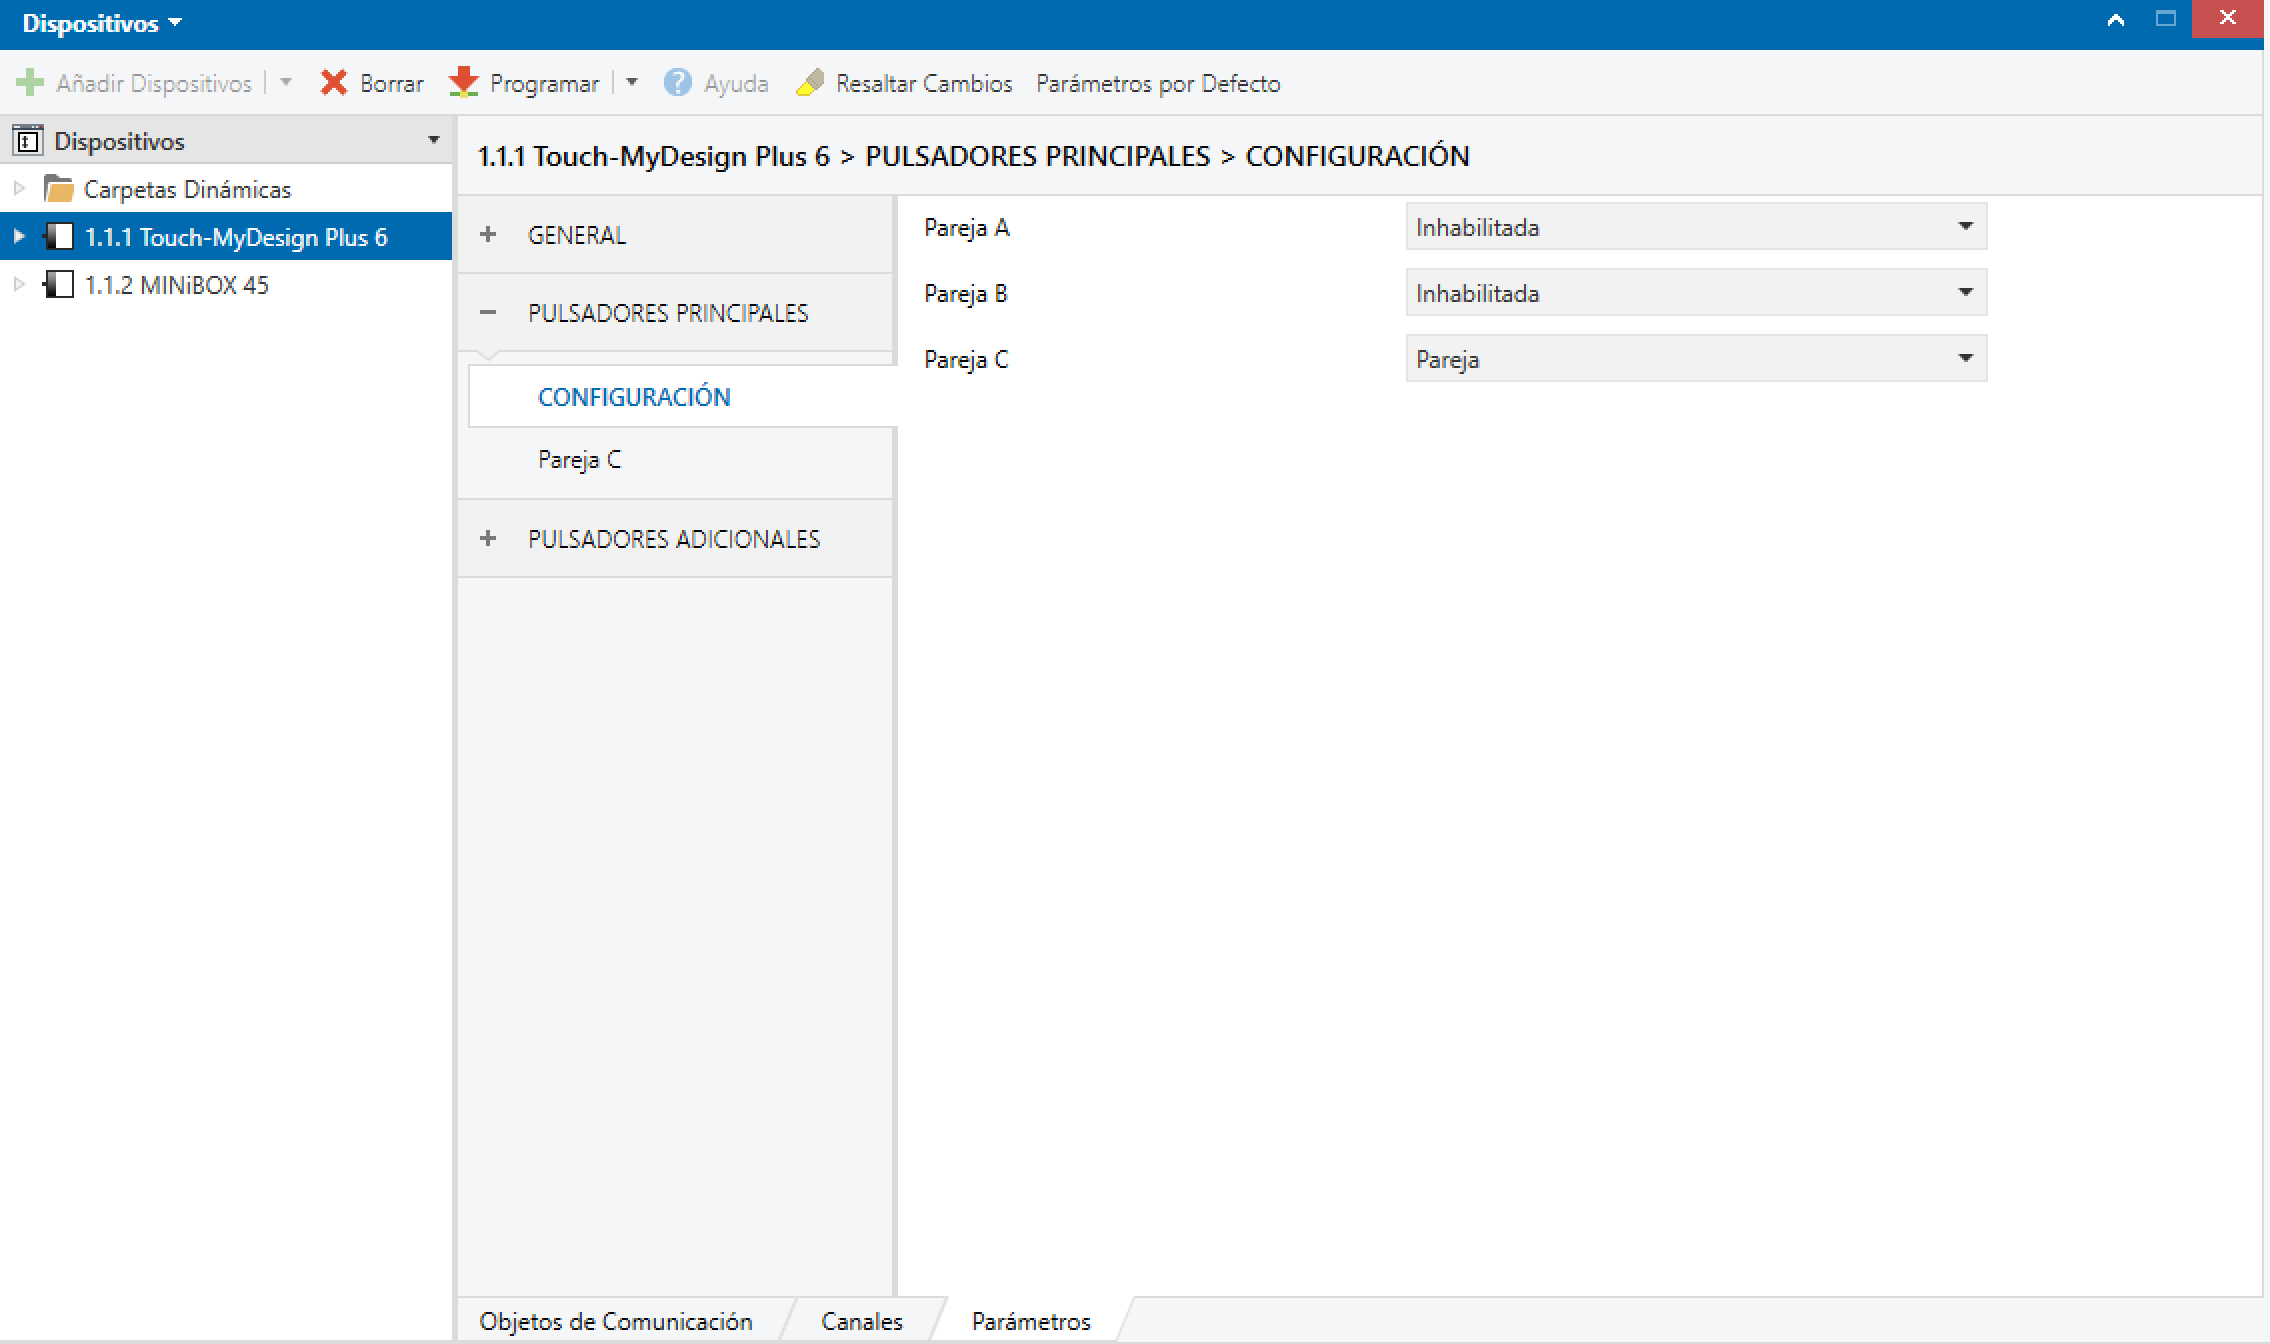
\includegraphics[width = 1.00\textwidth]{Imagenes/img36}
 		\captionof{figure}{\label{fig:IPN}Configurando dispositivo \textbf{Touch-MyDesing Plus 6} (I).} 
	\end{center} 
\end{figure}

\begin{figure}[H]
	\begin{center}
	 		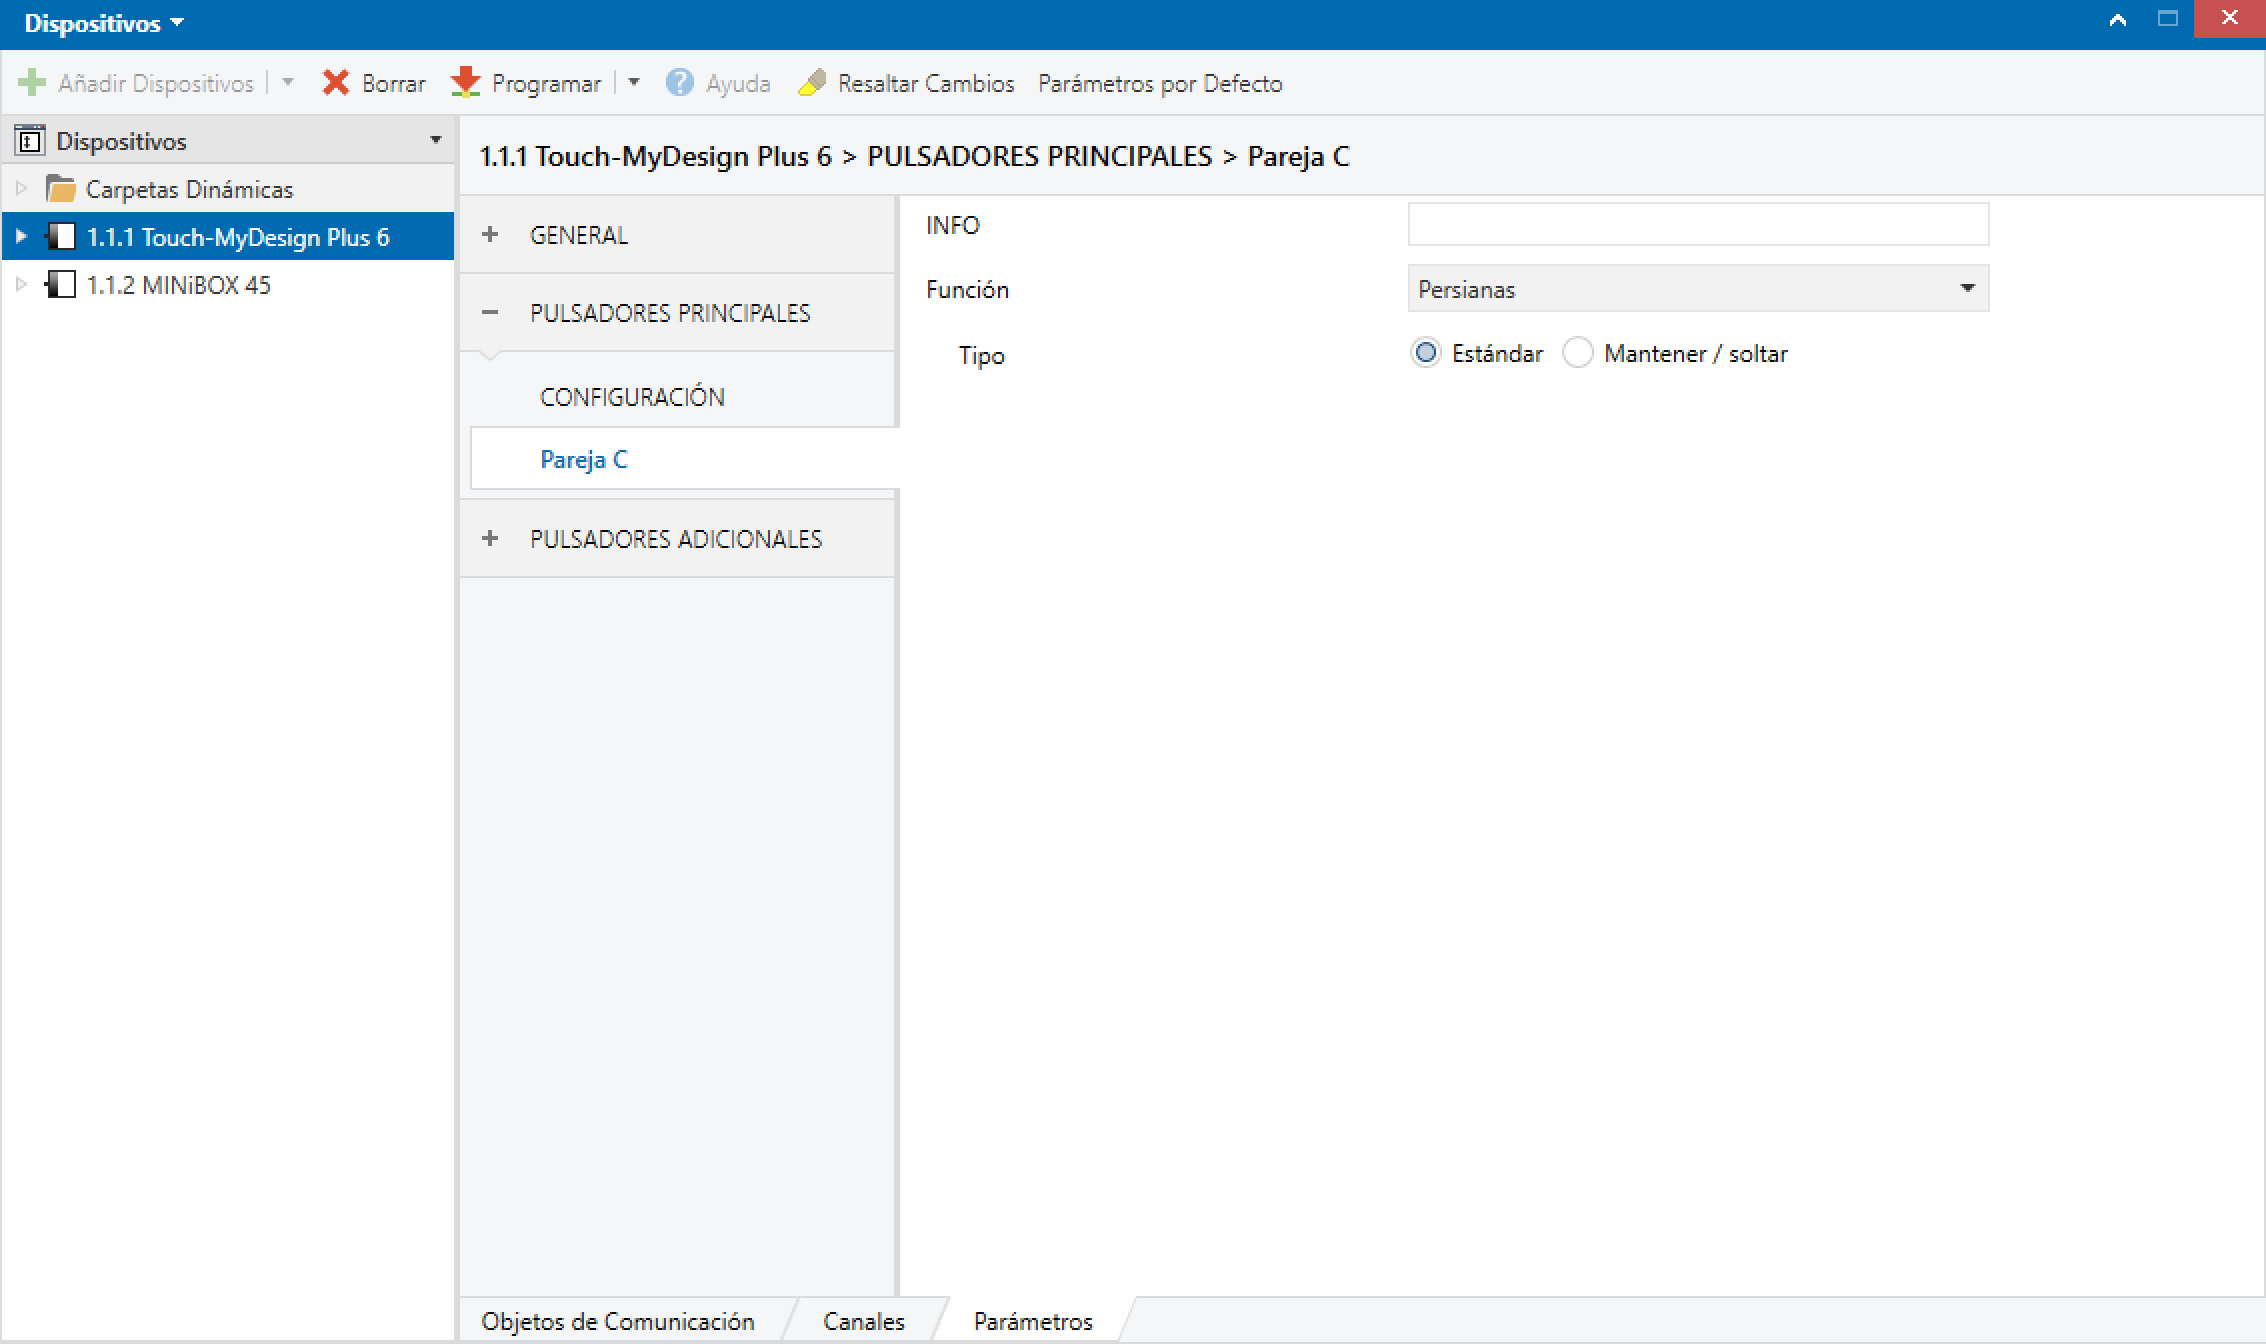
\includegraphics[width = 1.00\textwidth]{Imagenes/img37}
 		\captionof{figure}{\label{fig:IPN}Configurando dispositivo \textbf{Touch-MyDesing Plus 6} (II).} 
	\end{center} 
\end{figure}

Comenzaremos activando las salidas para el dispositivo \textbf{MINiBOX 45} y habilitando el Canal A como ``Canal persiana''. A continuación le estableceremos a dicho canal el tiempo que empleará tanto para subir como para bajar así como el tiempo de seguridad. Las funciones serán dejadas las que tiene por defecto. \\

\begin{figure}[H]
	\begin{center}
	 		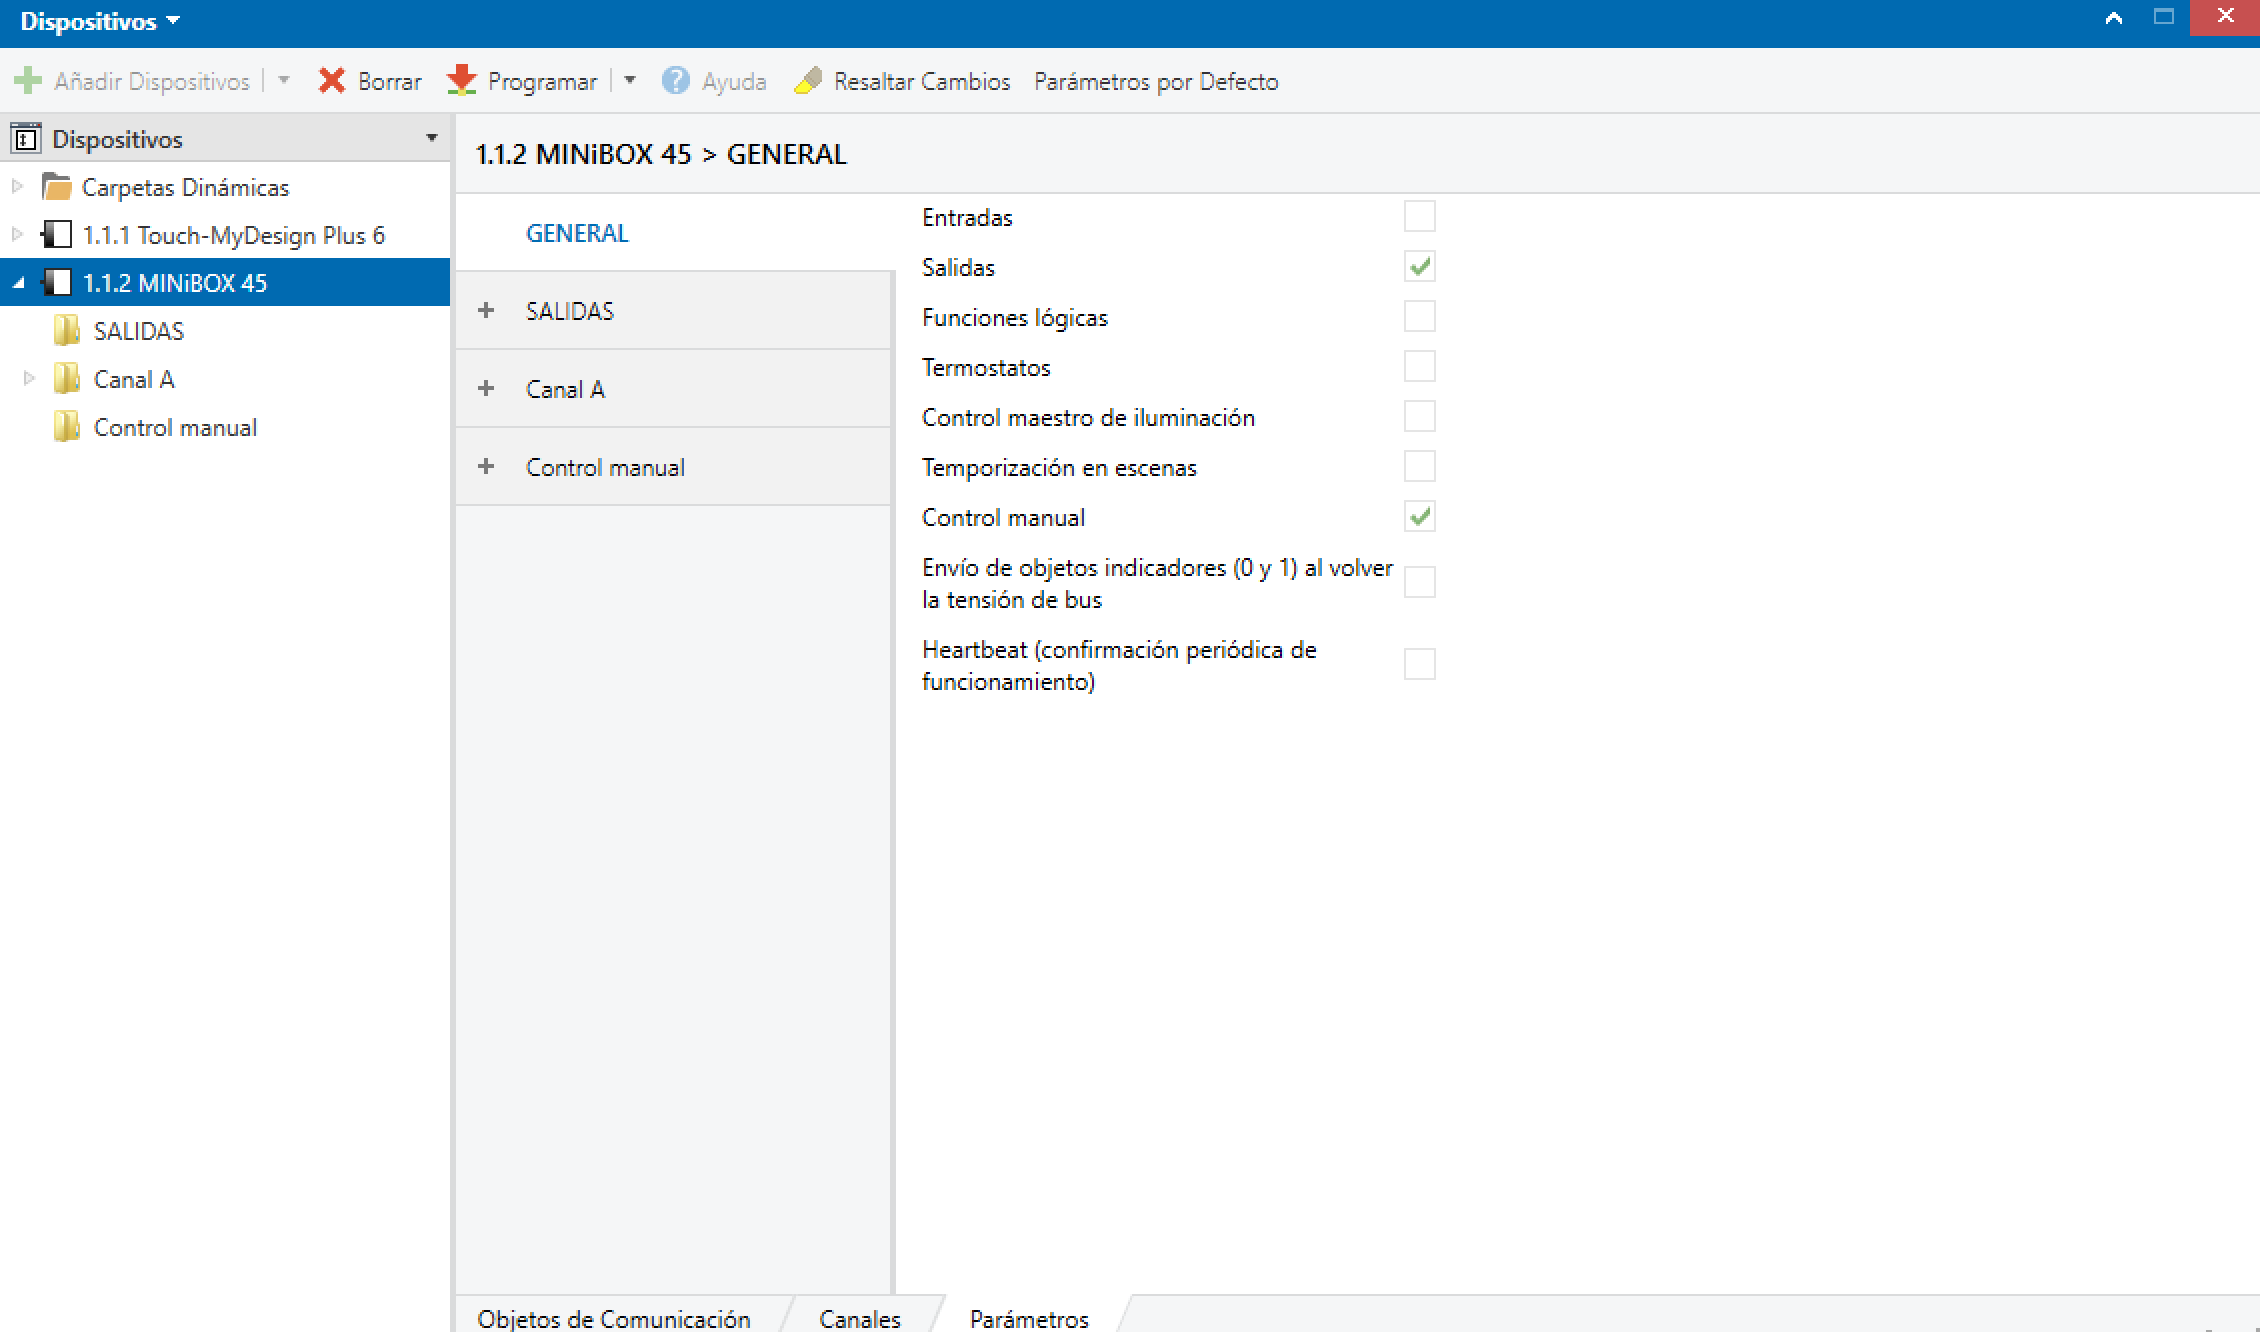
\includegraphics[width = 1.00\textwidth]{Imagenes/img38}
 		\captionof{figure}{\label{fig:IPN}Configurando dispositivo \textbf{MINiBOX 45} (I).} 
	\end{center} 
\end{figure}

\begin{figure}[H]
	\begin{center}
	 		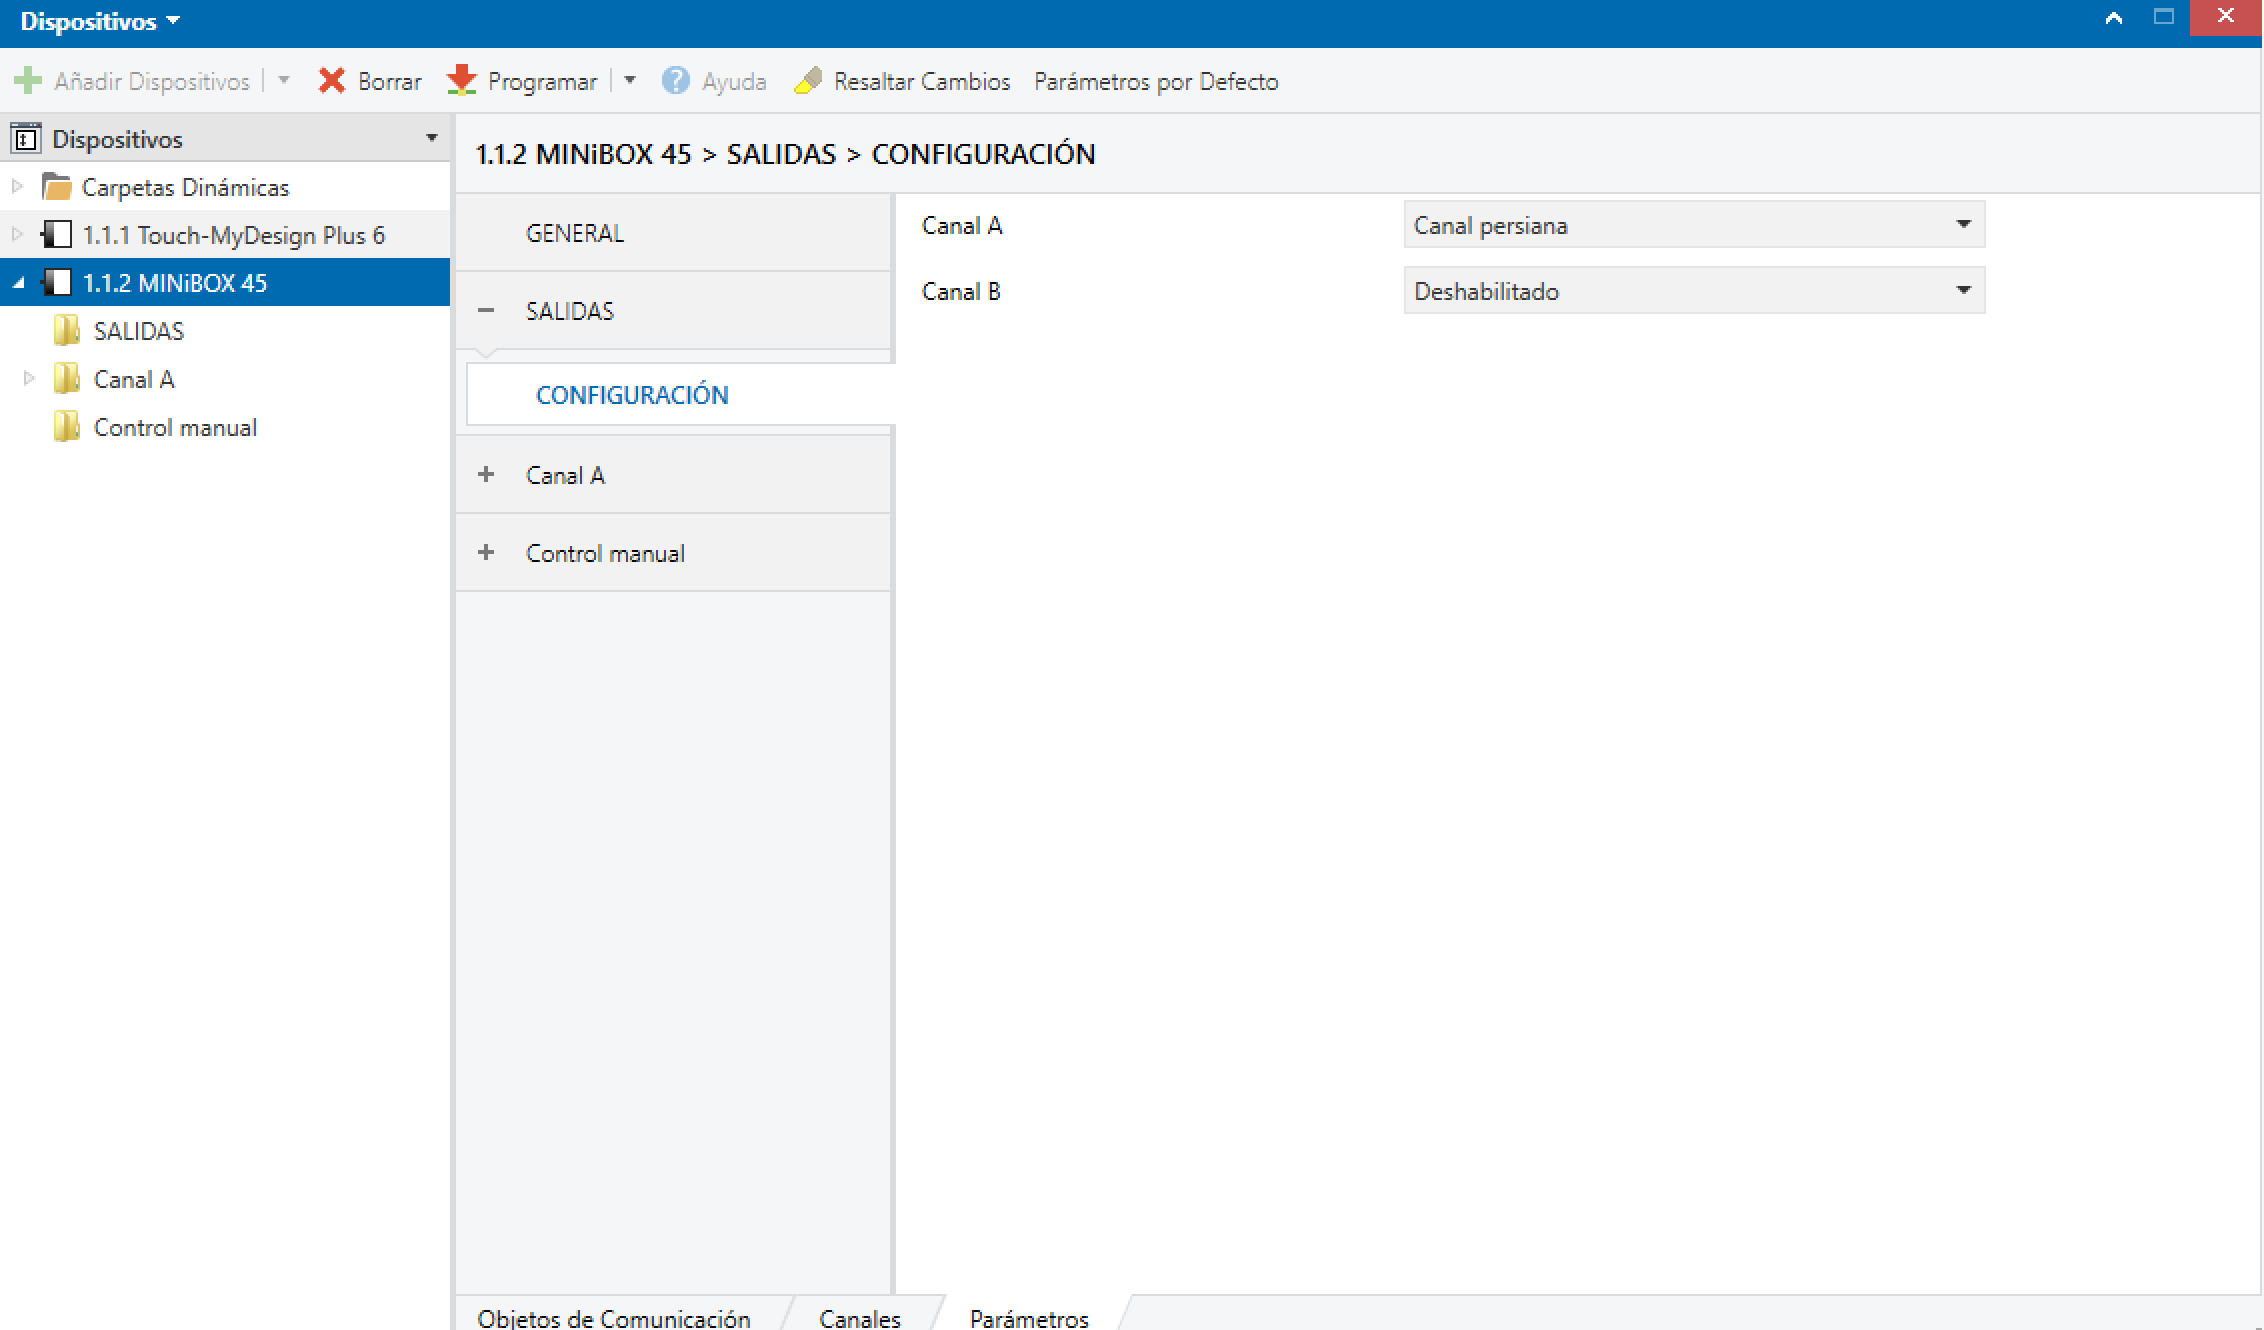
\includegraphics[width = 1.00\textwidth]{Imagenes/img39}
 		\captionof{figure}{\label{fig:IPN}Configurando dispositivo \textbf{MINiBOX 45} (II).} 
	\end{center} 
\end{figure}

\begin{figure}[H]
	\begin{center}
	 		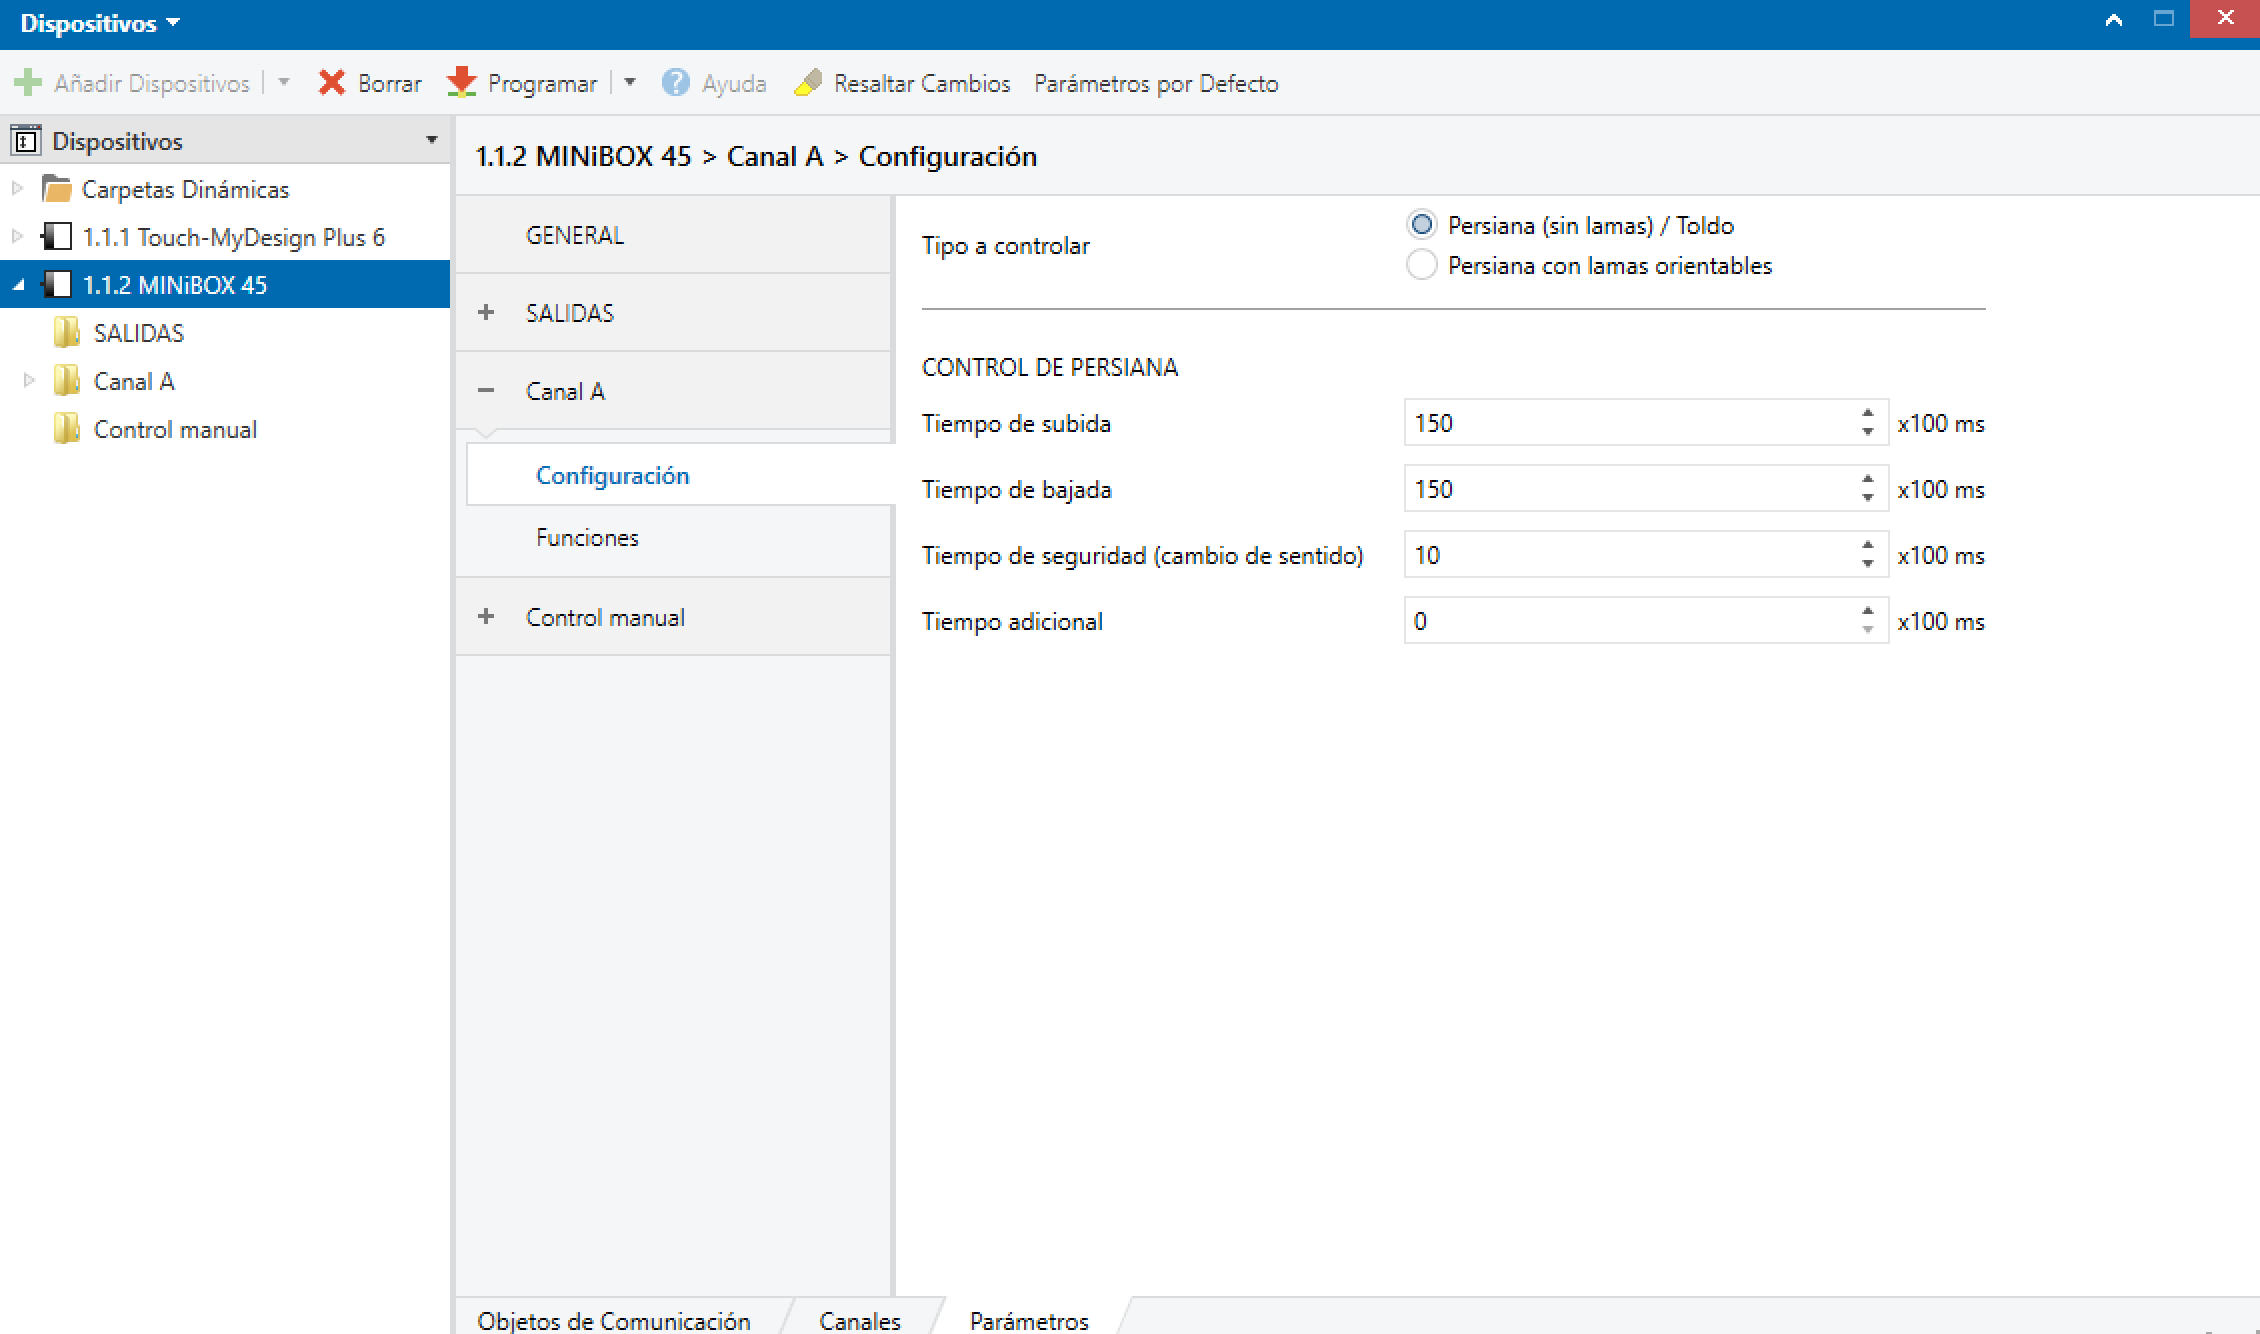
\includegraphics[width = 1.00\textwidth]{Imagenes/img40}
 		\captionof{figure}{\label{fig:IPN}Configurando dispositivo \textbf{MINiBOX 45} (III).} 
	\end{center} 
\end{figure}


Pasamos ahora a definir los grupos de direcciones para posteriormente añadirles los objetos de comunicación necesarios. \\

\begin{figure}[H]
	\begin{center}
	 		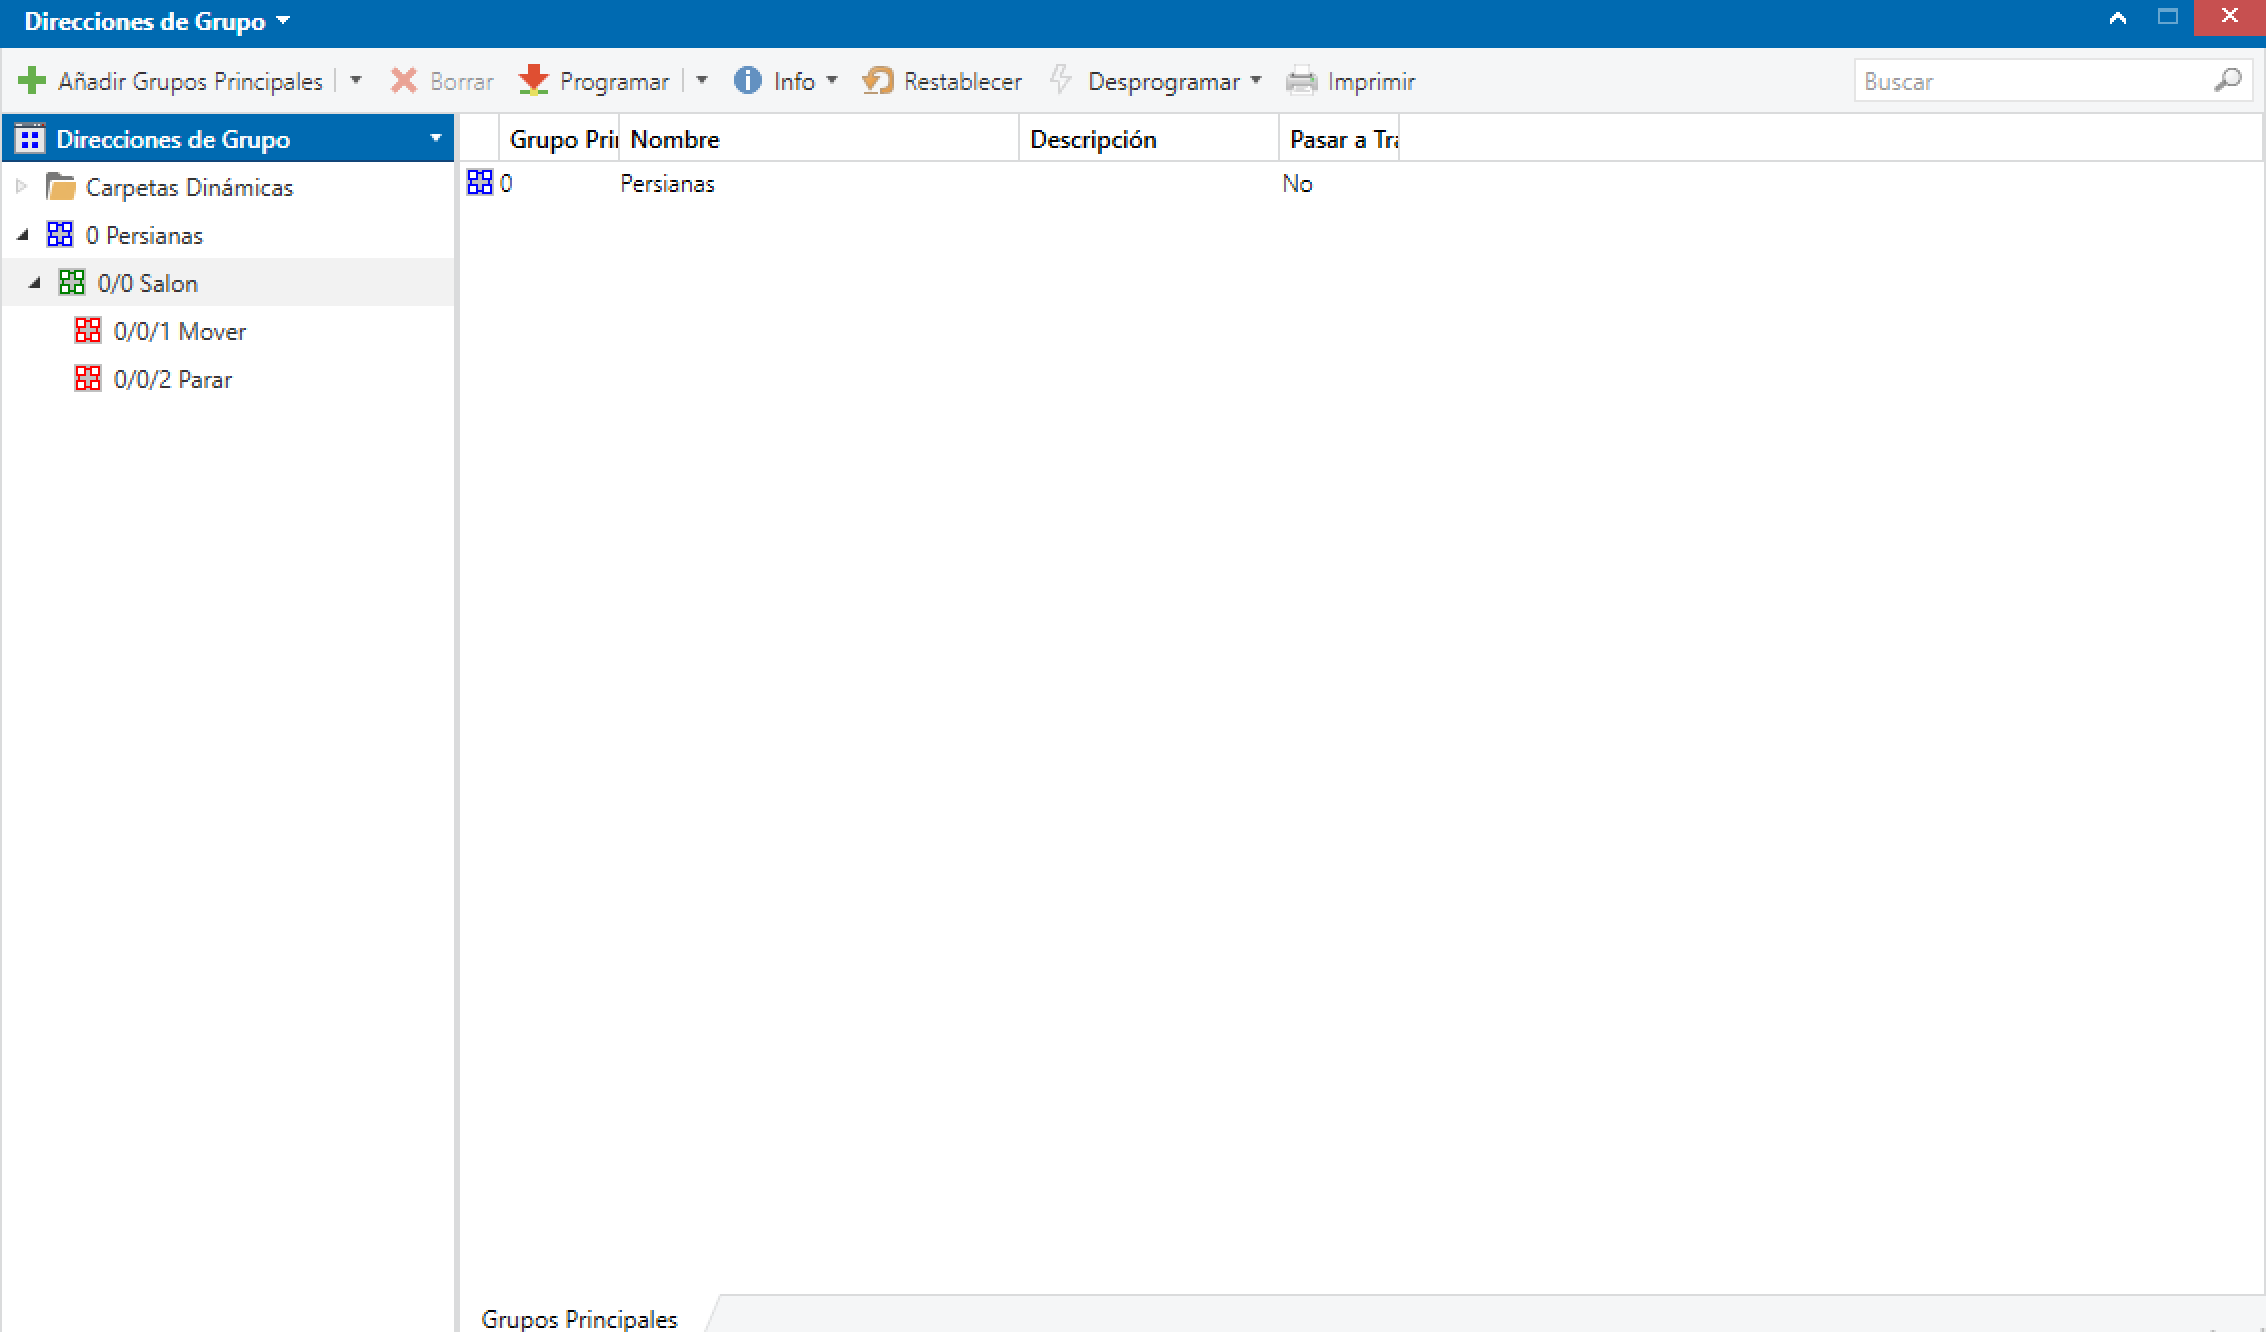
\includegraphics[width = 1.00\textwidth]{Imagenes/img41}
 		\captionof{figure}{\label{fig:IPN}Definiendo direcciones de grupo.} 
	\end{center} 
\end{figure}


La dirección de grupo \textbf{Mover} tendrá el objeto de comunicación ``Subir/bajar persiana'' del teclado \textbf{Touch-MyDesing Plus 6} para el pulsado de las teclas y el objeto de comunicación \textbf{Mover} del dispositivo \textbf{MINiBOX 45} para accionar el relé que mueve las persianas. \\

\begin{figure}[H]
	\begin{center}
	 		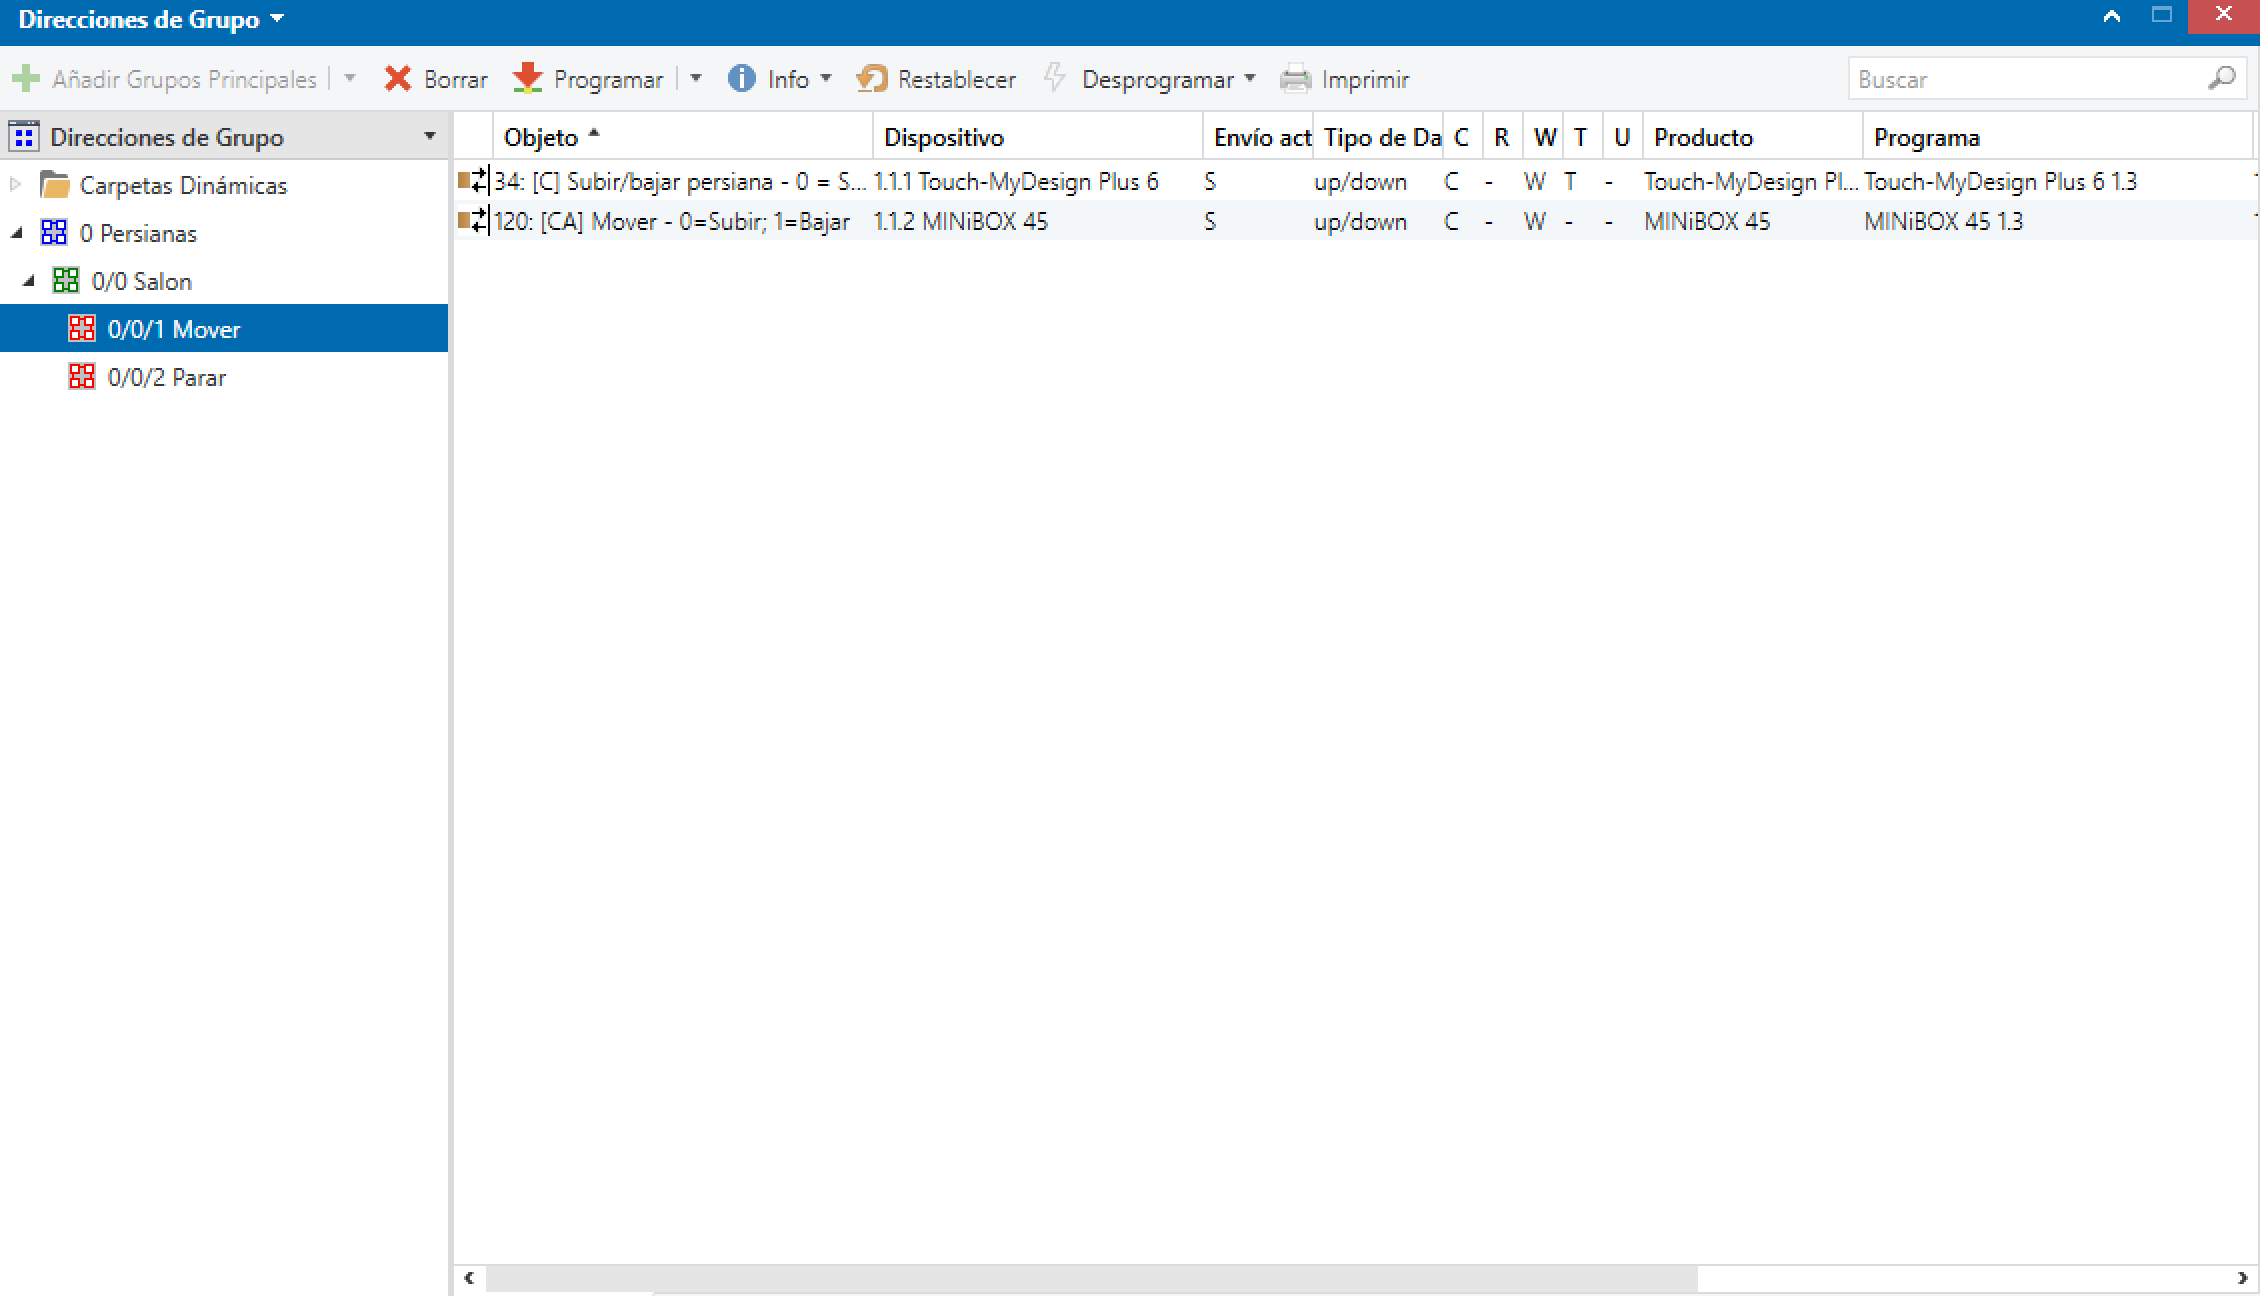
\includegraphics[width = 1.00\textwidth]{Imagenes/img42}
 		\captionof{figure}{\label{fig:IPN}Añdiendo objetos de comunicación a la dirección de grupo \textbf{Mover}.} 
	\end{center} 
\end{figure}

Para la dirección de grupo \textbf{Parar} añadiremos también objetos de comunicación de ambos dispositivos. Del teclado \textbf{Touch-MyDesing Plus 6} añadiremos el objeto de comunicación ``Detener persiana'' para hacer que se detengan las persianas, mientras que del \textbf{MINiBOX 45} añadiremos el objeto ``Parar'' para que el relé que las mueve se detenga. \\
 
 
 \begin{figure}[H]
	\begin{center}
	 		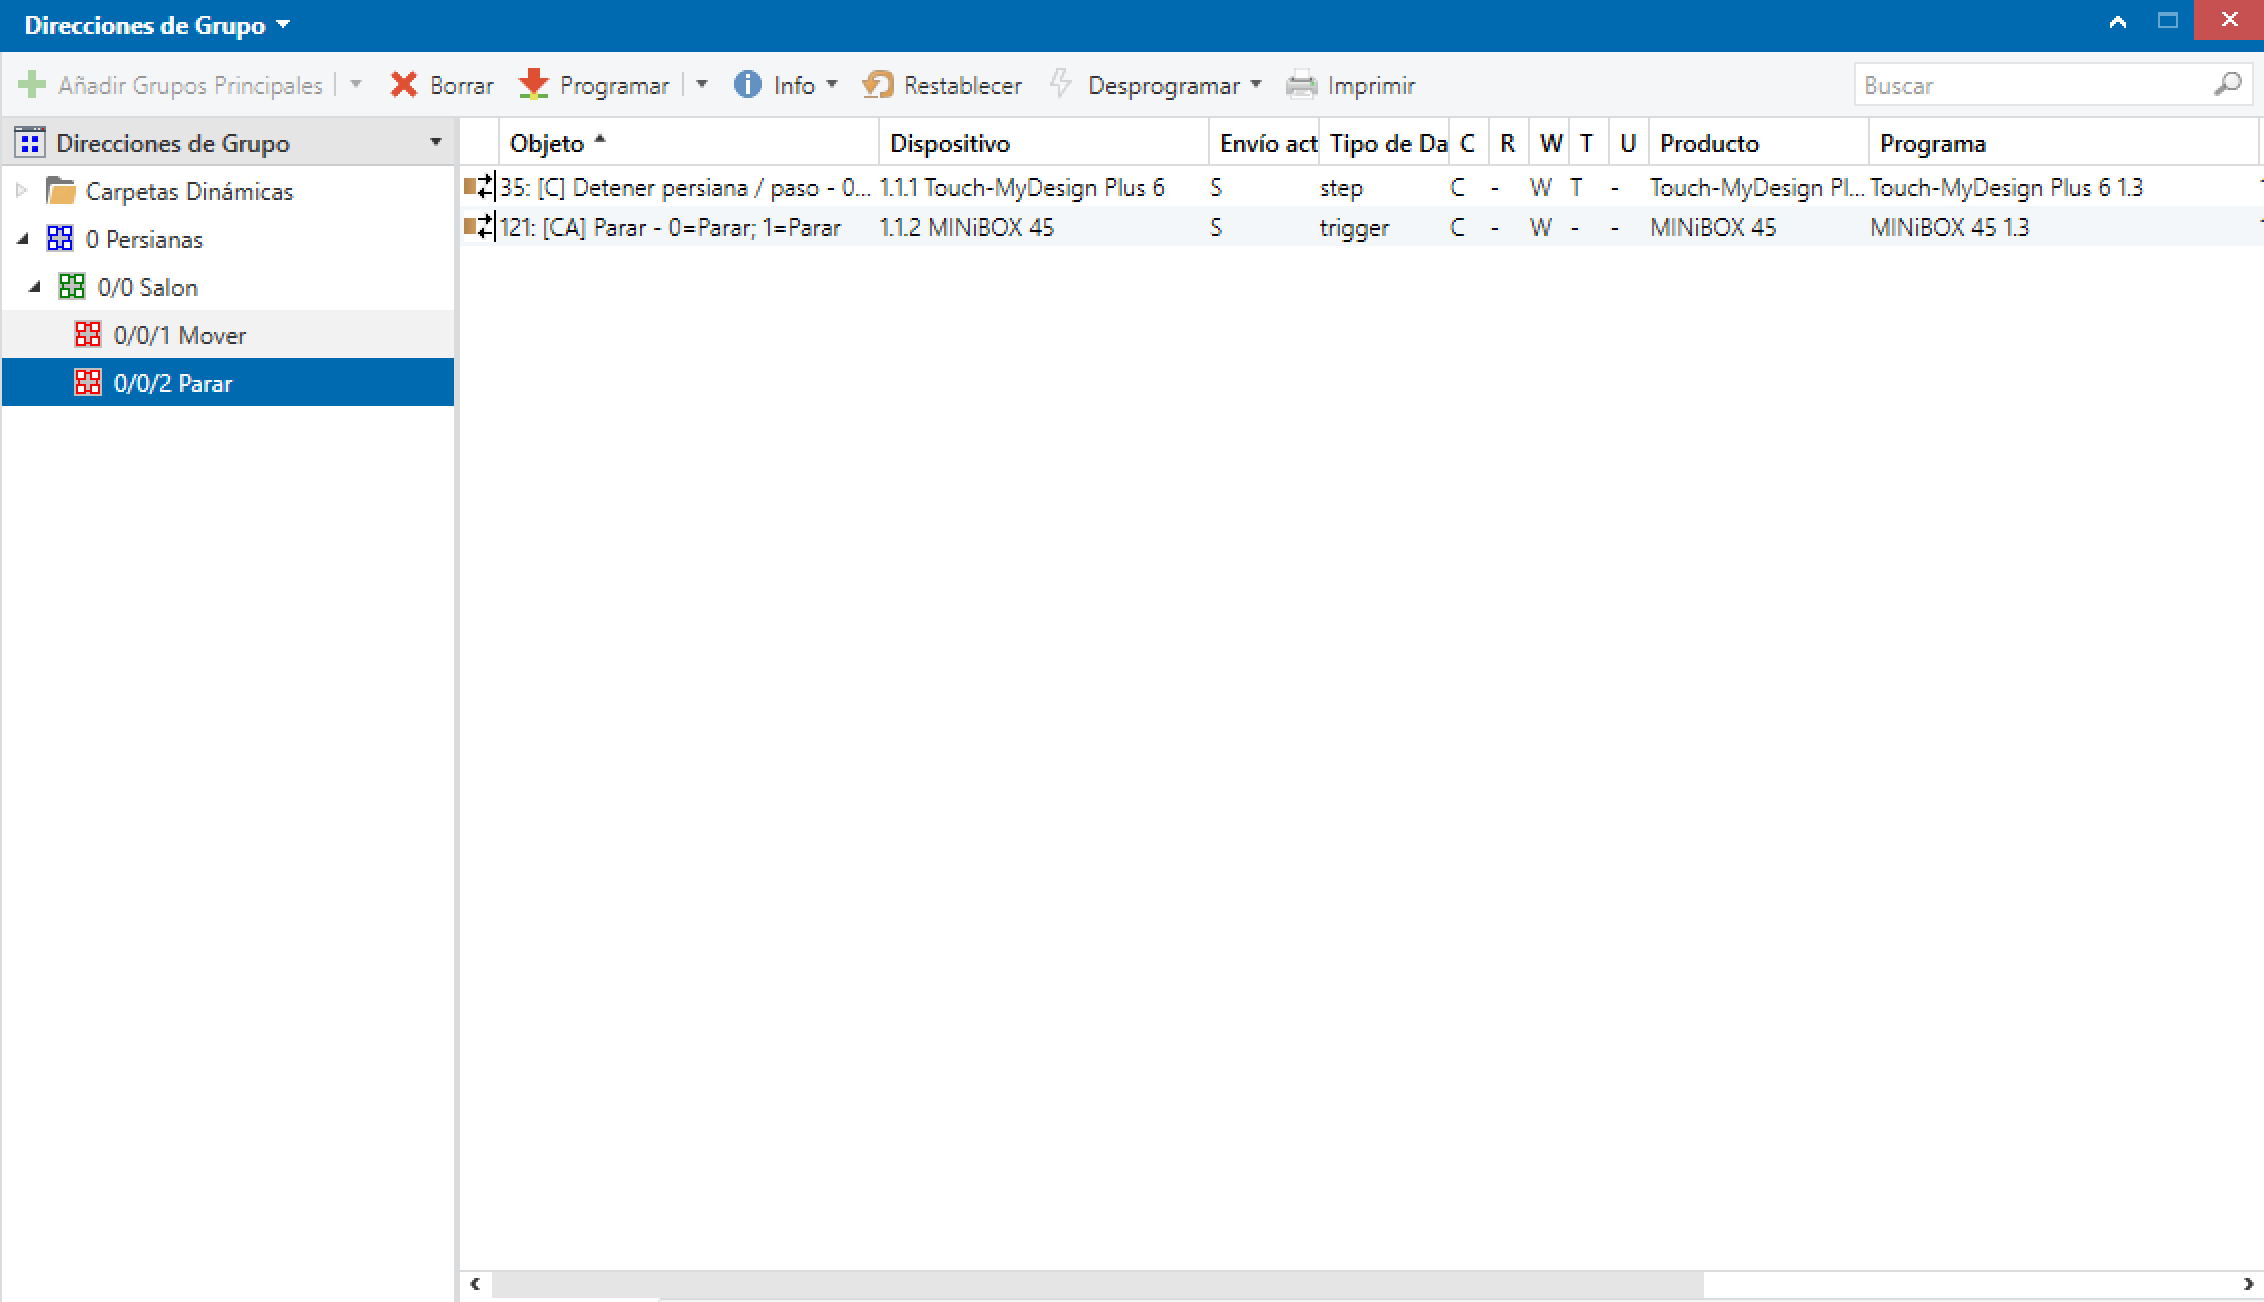
\includegraphics[width = 1.00\textwidth]{Imagenes/img43}
 		\captionof{figure}{\label{fig:IPN}Añdiendo objetos de comunicación a la dirección de grupo \textbf{Parar}.} 
	\end{center} 
\end{figure}

Con el sistema KNX configurado ya es posible programarlo para comprobar sus resultados como se pudo ver en el laboratorio de prácticas.\\


\section{Práctica 5. Uso de un panel táctil.} 
Como se mencionó anteriormente, esta práctica se realizó conjuntamente con la práctica 3 del \textbf{Control de temperatura}.\\

\end{document}

